\documentclass[final]{article}
\usepackage[utf8]{inputenc}
\usepackage[notref,notcite]{showkeys}
\usepackage{amsmath,amssymb,amsthm,amsfonts}
\usepackage{graphics}
\usepackage{graphicx,epsfig}
\usepackage{doc}
\usepackage{color}
% \usepackage{natbib}
\numberwithin{equation}{section}
\usepackage{multirow}
\usepackage{fancyvrb}
\usepackage{subfig}
\usepackage{outlines}
\usepackage{listings}
\usepackage{xcolor, xparse}
\usepackage{realboxes}
\usepackage[hmargin=1in,vmargin=1in]{geometry}

\usepackage{float}

\graphicspath{ {./figures/} }

%%%%%%%%%%%%%%%%%%%%%%%%%%%%%%%%%%%%%%%%%%%
% definition of the remark style
%%%%%%%%%%%%%%%%%%%%%%%%%%%%%%%%%%%%%%%%%%%
\newtheoremstyle{remarkStyle}% name
  {10pt}% Space above
  {10pt}% Space below
  {}% Body font
  {}% Indent amount
  {\bf}% Theorem head font
  {:}% Punctuation after theorem head
  {\newline}% Space after theorem head
  {}% Theorem head spec
%declaring the style to be used
\theoremstyle{remarkStyle}
\newtheorem{remark}{Remark}

%%%%%%%%%%%%%%%%%%%%%%%%%%%%%%%%%%%%%%%%%%%

\definecolor{codegreen}{rgb}{0,0.6,0}
\definecolor{codegray}{rgb}{0.5,0.5,0.5}
\definecolor{codepurple}{rgb}{0.58,0,0.82}
\definecolor{backcolour}{rgb}{0.95,0.95,0.92}

\definecolor{green}{rgb}{0.,0.5,0.0}
\lstdefinestyle{mystyle}{
    backgroundcolor=\color{backcolour},   
    commentstyle=\color{codegreen},
    keywordstyle=\color{magenta},
    numberstyle=\tiny\color{codegray},
    stringstyle=\color{codepurple},
    basicstyle=\ttfamily\footnotesize,
    breakatwhitespace=false,         
    breaklines=true,                 
    captionpos=b,                    
    keepspaces=true,                 
    numbers=left,                    
    numbersep=5pt,                  
    showspaces=false,                
    showstringspaces=false,
    showtabs=false,                  
    tabsize=2
}


\lstset{style=mystyle}

\DeclareDocumentCommand{\clist}{v}{%
    \Colorbox{backcolour}{\csname lstinline\endcsname!#1!}%
}

\title{2.077 Final Project}
\author{Jorge Nin}
\date{\today}



\makeatletter
\def\@maketitle{%
  \newpage
  \null
  
  \vskip 2em%
  \begin{center}%
    \vspace*{\fill}
  \let \footnote \thanks
    {\Huge \@title \par}%
    \vskip 1em%
    {\huge Plasticity \par}%
    \vskip 1.5em%
    {\large
      \lineskip .5em%
      \begin{tabular}[t]{c}%
        \@author
      \end{tabular}\par}%
    \vskip 1em%
    {\large \@date}%
  \end{center}%
  \vspace*{\fill}
  \par
  \vskip 1.5em}
\makeatother




\begin{document}

\maketitle
\thispagestyle{empty}
\pagebreak
\tableofcontents
\pagebreak
\section{Introduction and Background}

This document will help install and setup a docker instance of FEniCSx used for 2.077.
We will be using FEniCSx 0.8.0 Dev.


While this is an unstable version right now it is the only version with good Quadrature Element support.
If you want the stable version just pull the image:

\begin{lstlisting}[language=bash, caption=Docker Pull Command]
  > docker pull jorgenin/dolfinx-2.077:v0.7
\end{lstlisting}


These instructions are made specifically with Mac OS in mind, but after installing docker, the process should be platform independent.




% \begin{figure}[H]
%   \centering
%   \subfloat[\centering label 1]{{\includegraphics[width=6cm]{Test1.png} }}%
%   \qquad
%   \subfloat[\centering label 2]{{\includegraphics[width=6cm]{Test2.png} }}%
%   \caption{2 Figures side by side}%
%   \label{fig:example}%
% \end{figure}







\section{Docker}

 {\LARGE \textcolor{red}{WARNING: Please backup your data. Data stored in a container may be lost at any time. Use git or a volume to ensure your data is well protected.}}


\subsection{What is Docker}

Docker is a platform that uses containerization technology to simplify
the deployment and management of software applications. In the context of
software development, especially for complex engineering applications like FeniCSx,
Docker offers several advantages:

\begin{outline}
  \1 Containerization:

  \2 Containers are isolated environments where applications can run.
  They are lightweight because they share the host system's kernel (but not the OS itself)
  and are not burdened with the overhead of a virtual machine.
  \2 For FEniCSx, this means that each instance of the application runs in a consistent environment, irrespective of the underlying hardware or software configurations of the host system.


  \1 Consistency and Reproducibility:

  \2 Docker ensures that FEniCSX runs identically on every machine, avoiding the common "it works on my machine" problem in software development.

  \1 Ease of Distribution and Version Control:

  \2 Docker images (blueprints for containers) can be version-controlled and shared through Docker Hub or other registries, ensuring that all students and researchers access the same version of FEniCSX and it's dependencies.



\end{outline}

Because of these advantages, we will be using Docker to run FEniCSx.

\subsection{Installing Docker}
It is recommended that you install docker desktop for first time use. You can find the download here: \href{https://www.docker.com/products/docker-desktop}{Docker Desktop} and download the appropriate version for your operating system.
An account is not necessary for basic install and usage.

After downloading open up the image and drag it into the applications folder. Docker should now be installed.
\begin{figure}[H]
  \centering
  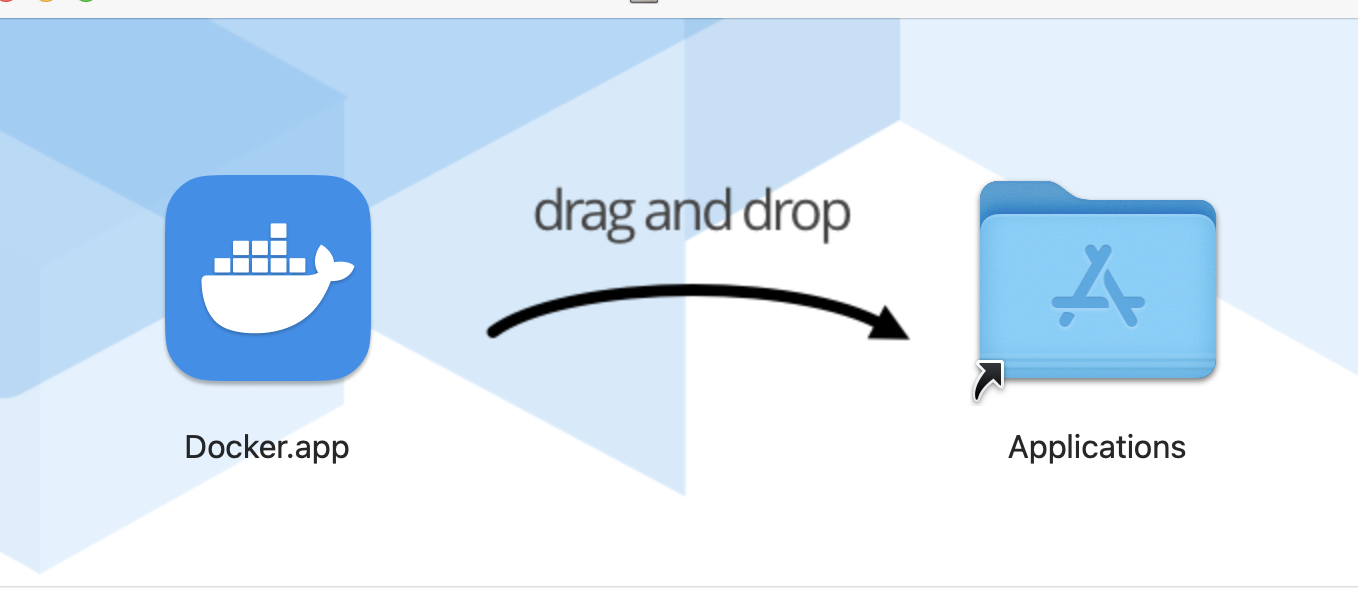
\includegraphics[width=0.7\textwidth]{DockerInstall.png}
  \caption{Docker install process}
\end{figure}

After docker has finished installing open up the docker desktop application.

The application may not instantly open. Insead it may be in the background, look at figure \ref{fig:open_docker} to see if you're docker is in the background.
\begin{figure}[H]
  \centering
  \subfloat[\centering Docker Open in the background]{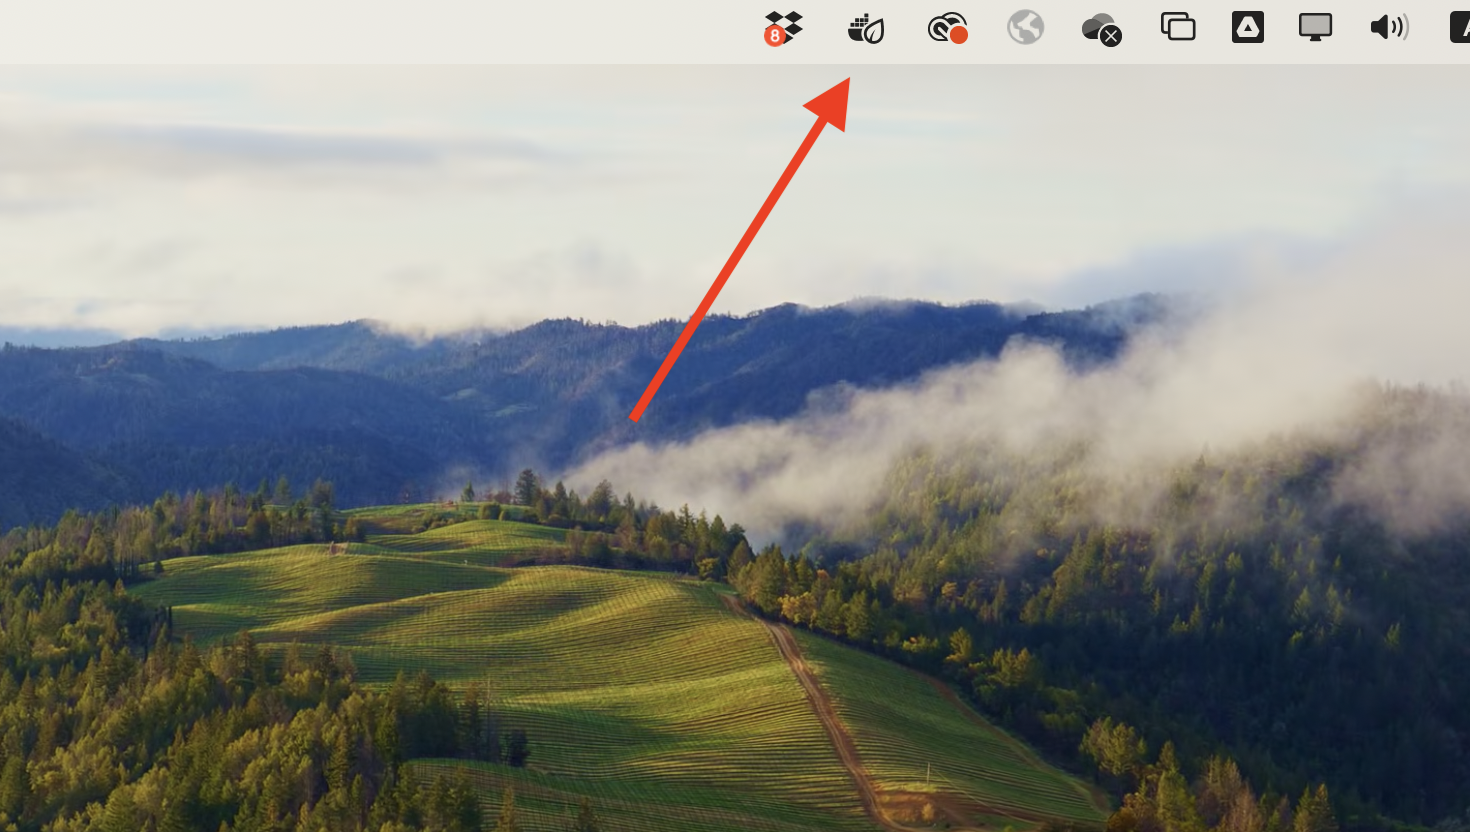
\includegraphics[width=0.5\textwidth]{DockerApp_open.png}}%
  \qquad
  \subfloat[\centering Clicking on the Docker Symbol]{{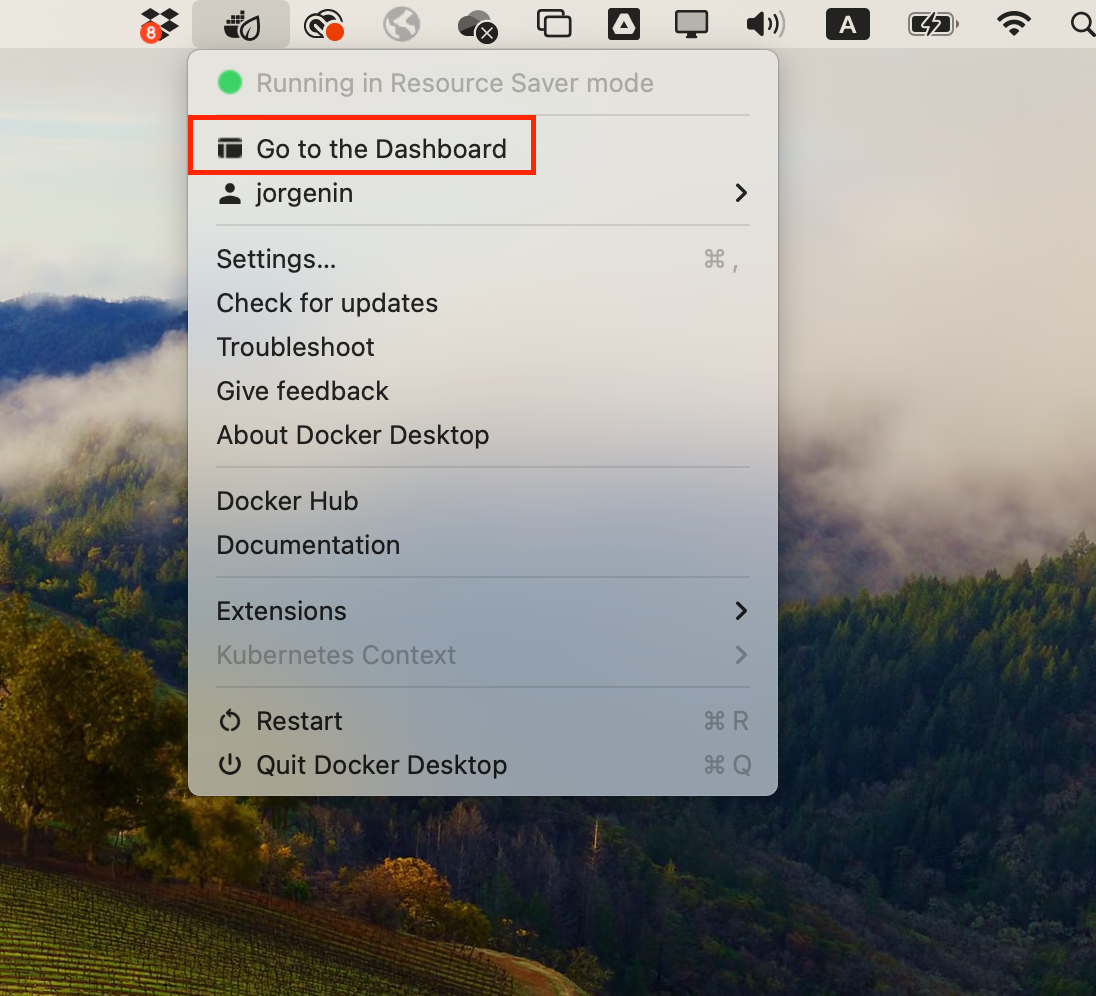
\includegraphics[width=0.3\textwidth]{OpenDockerApp.png}}}%
  \caption{How to check if docker is open in the background. Click on the "Go to dashboard" to open up docker.}%
  \label{fig:open_docker}%
\end{figure}

\subsection{Docker Layout}
Once docker is open you should see a window similar to this. This is the dashboard.


\begin{figure}[H]
  \centering
  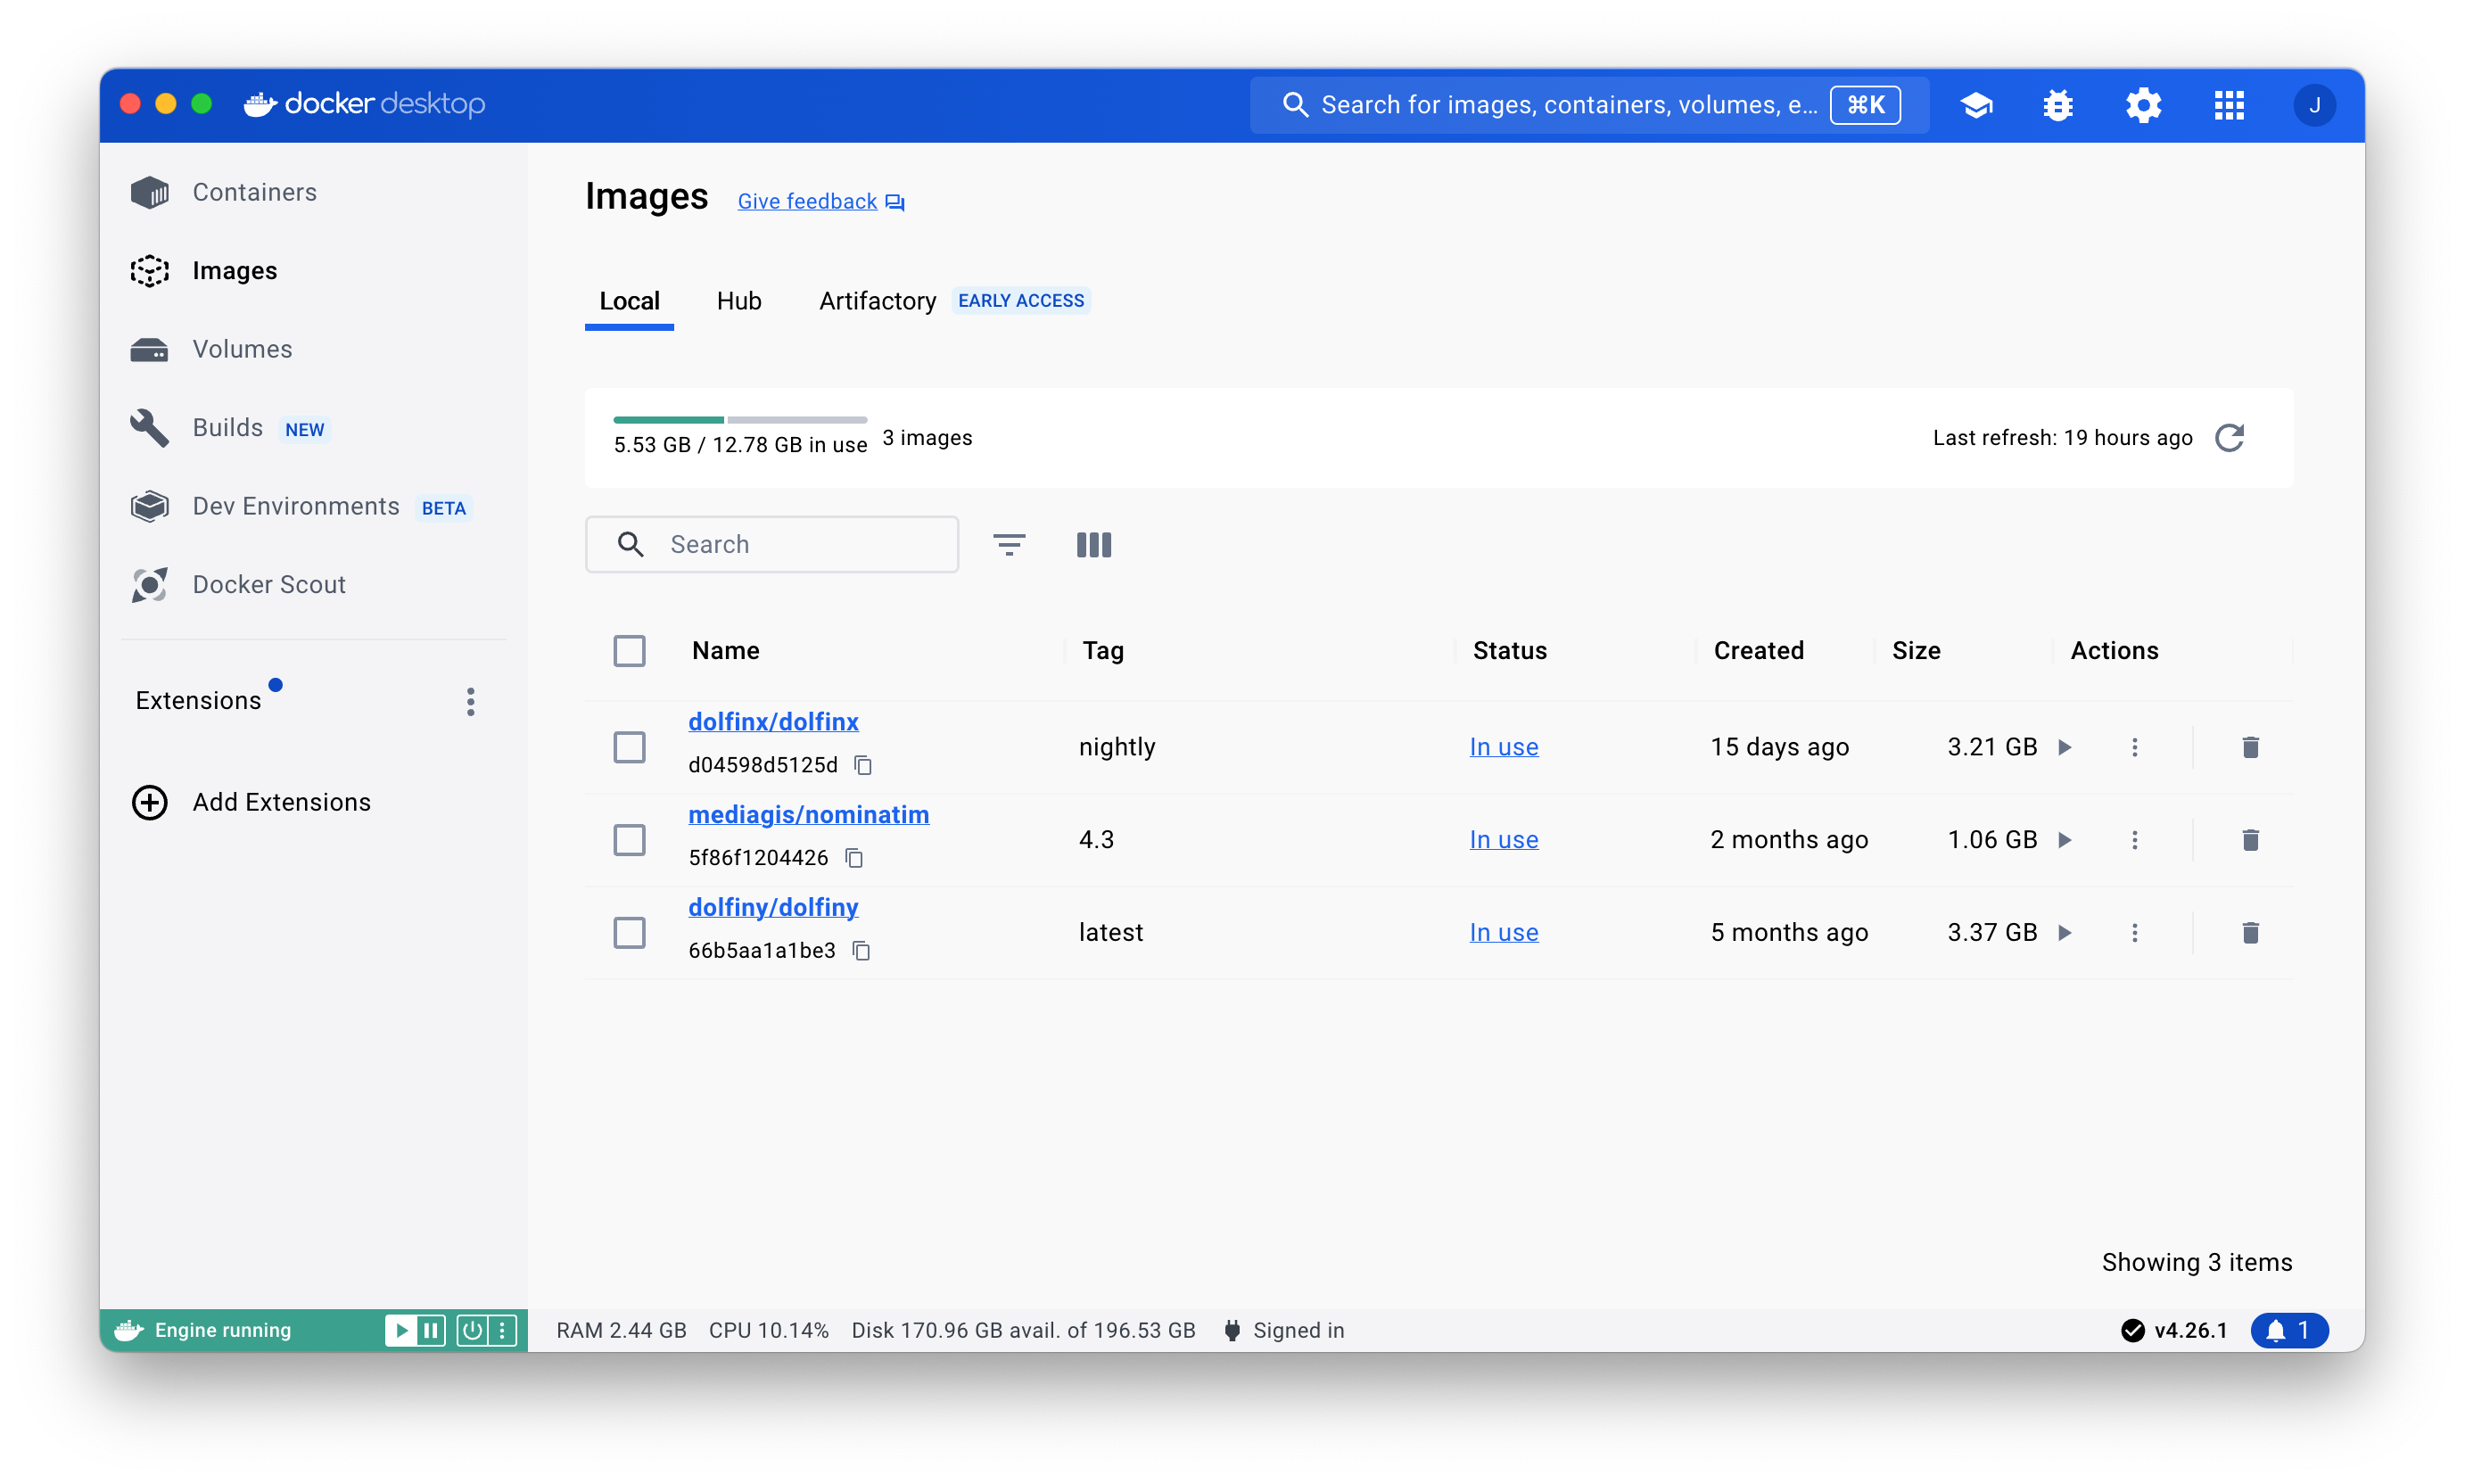
\includegraphics[width=0.7\textwidth]{DockerHomePage.png}
  \caption{ The Docker Dashboard}%
  \label{fig:docker_home}%
\end{figure}


There are multiple tabs but we will only be convering two of them. The Containers tab, and the images tab.

\subsubsection{Images}



\begin{figure}[H]
  \centering
  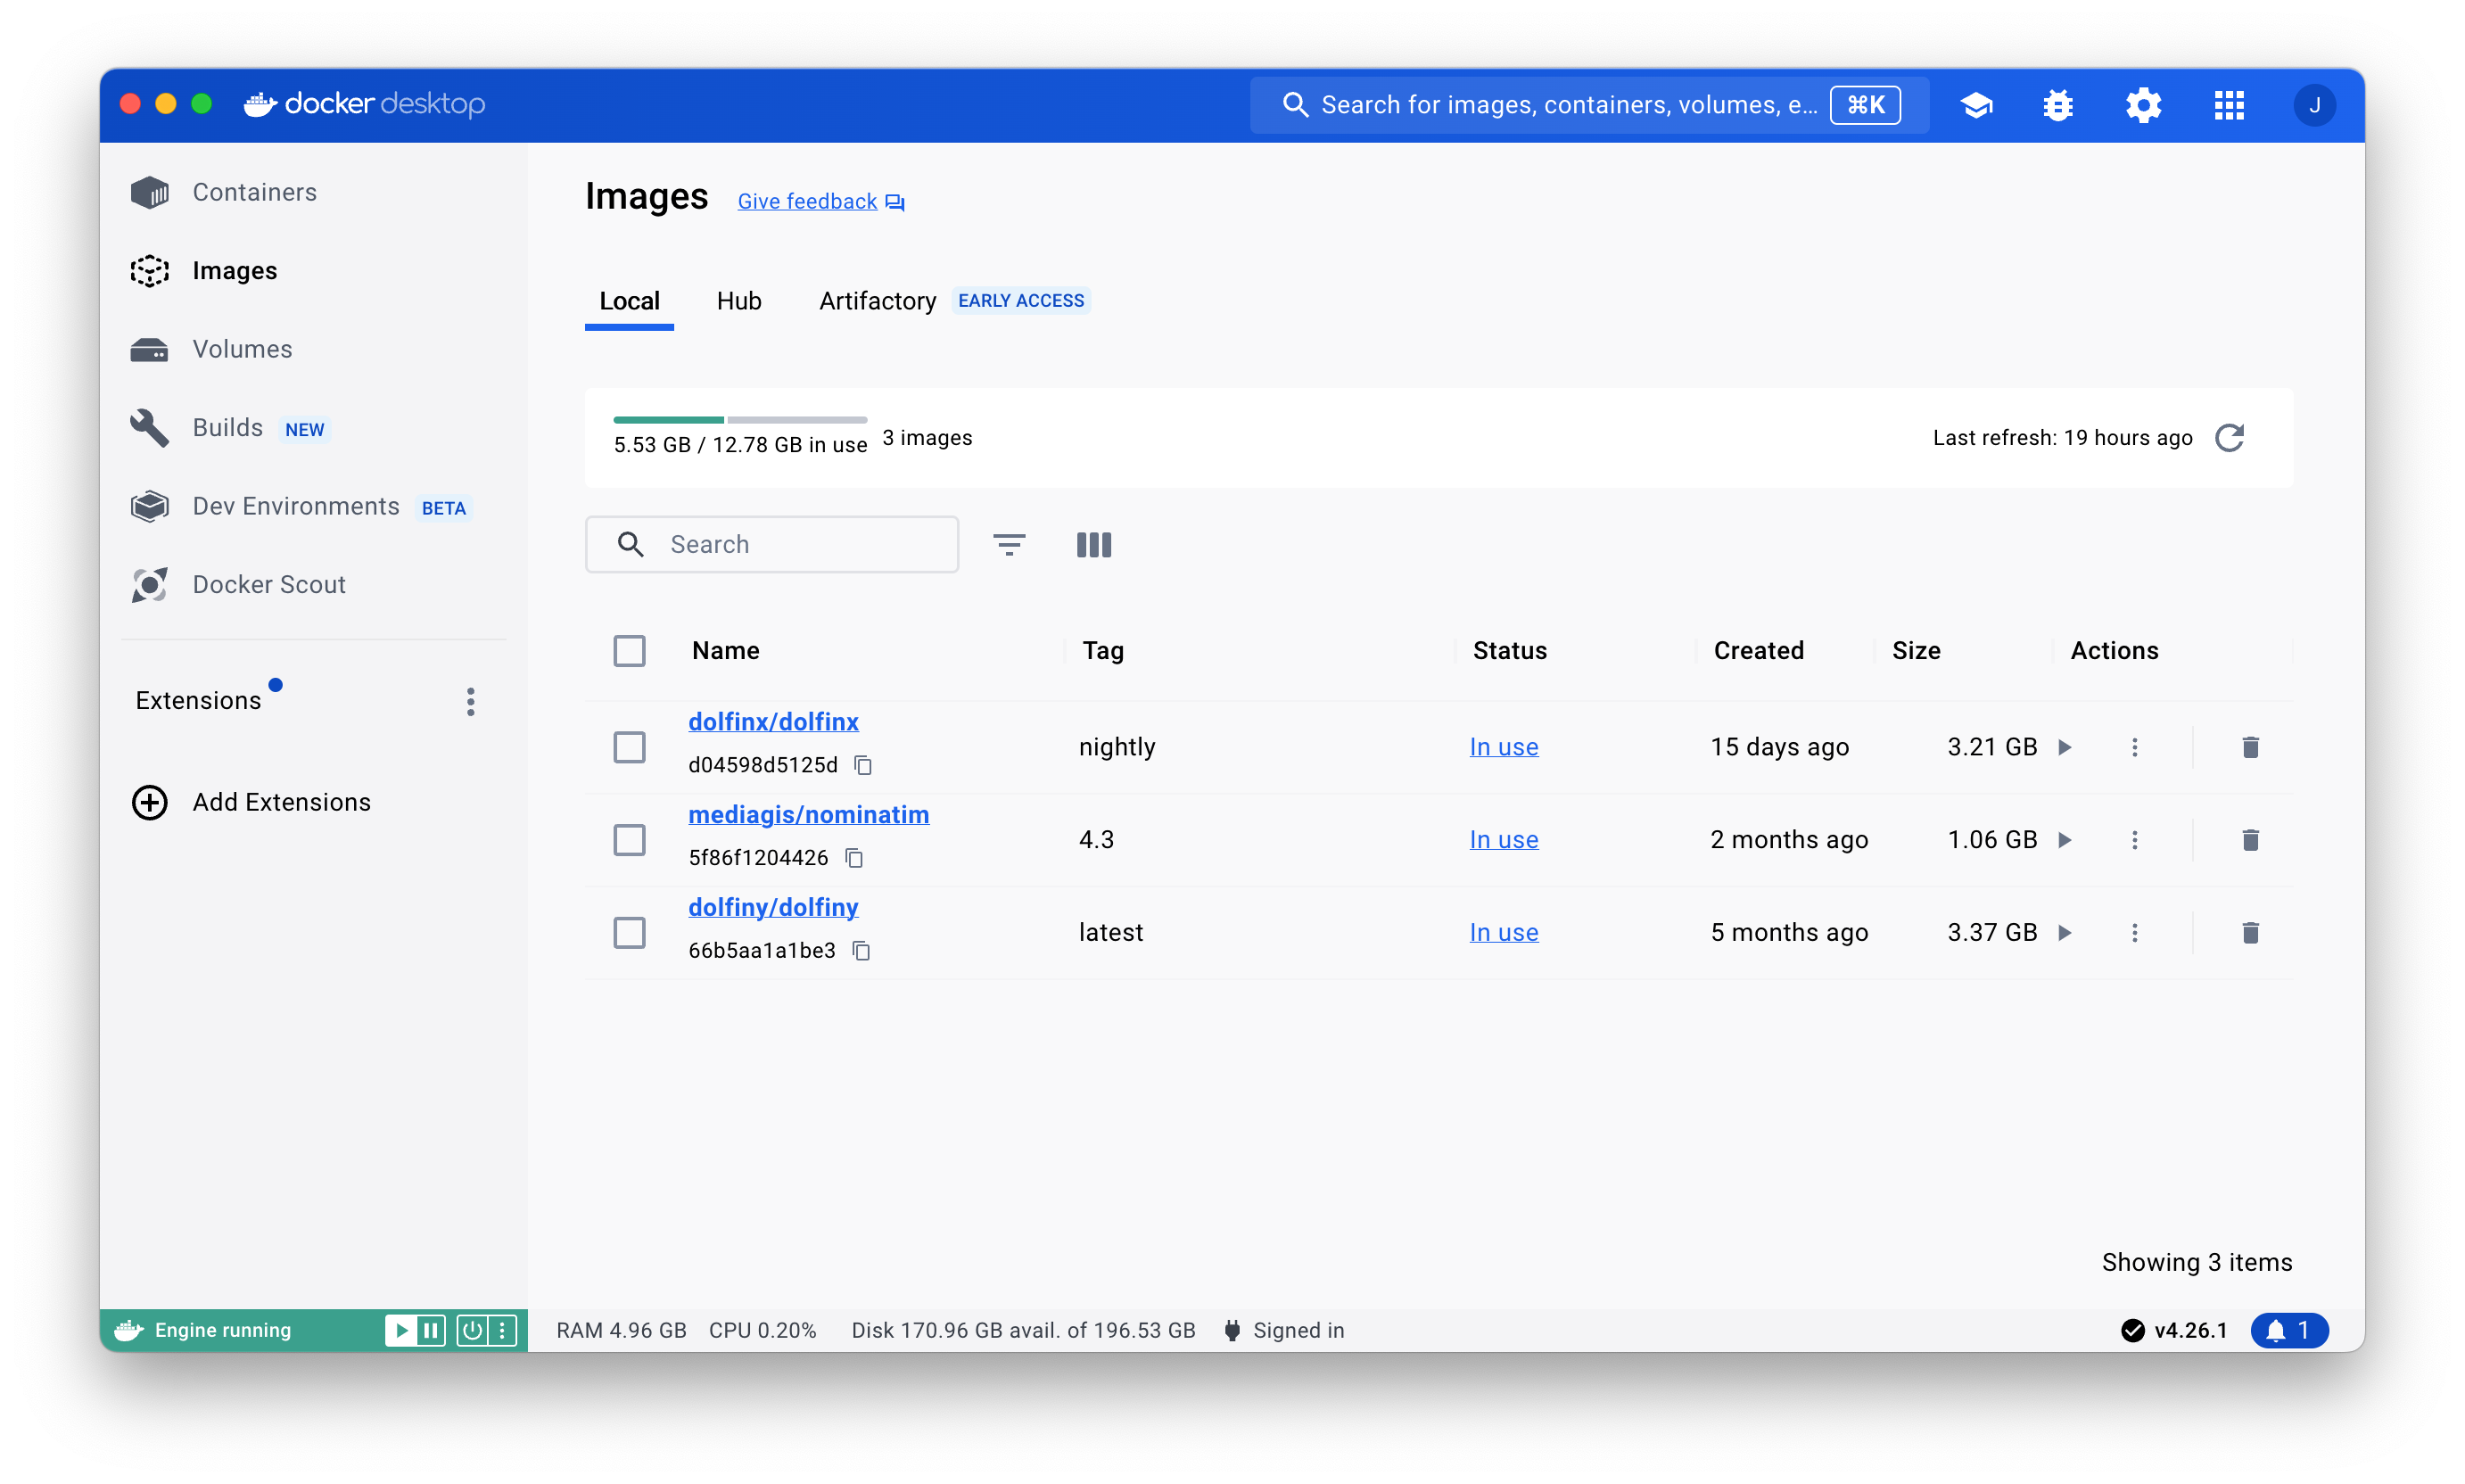
\includegraphics[width=0.7\textwidth]{DockerImages.png}
  \caption{ The Docker Images Tab}%
  \label{fig:docker_Images}%
\end{figure}

The docker images tab contains all of the Images you currently have installed. Image are essentially different operating sytems you can have. If you want to run multiple version of FEniCSx for example you could have multiple images of it.




\subsubsection{Containers}



\begin{figure}[H]
  \centering
  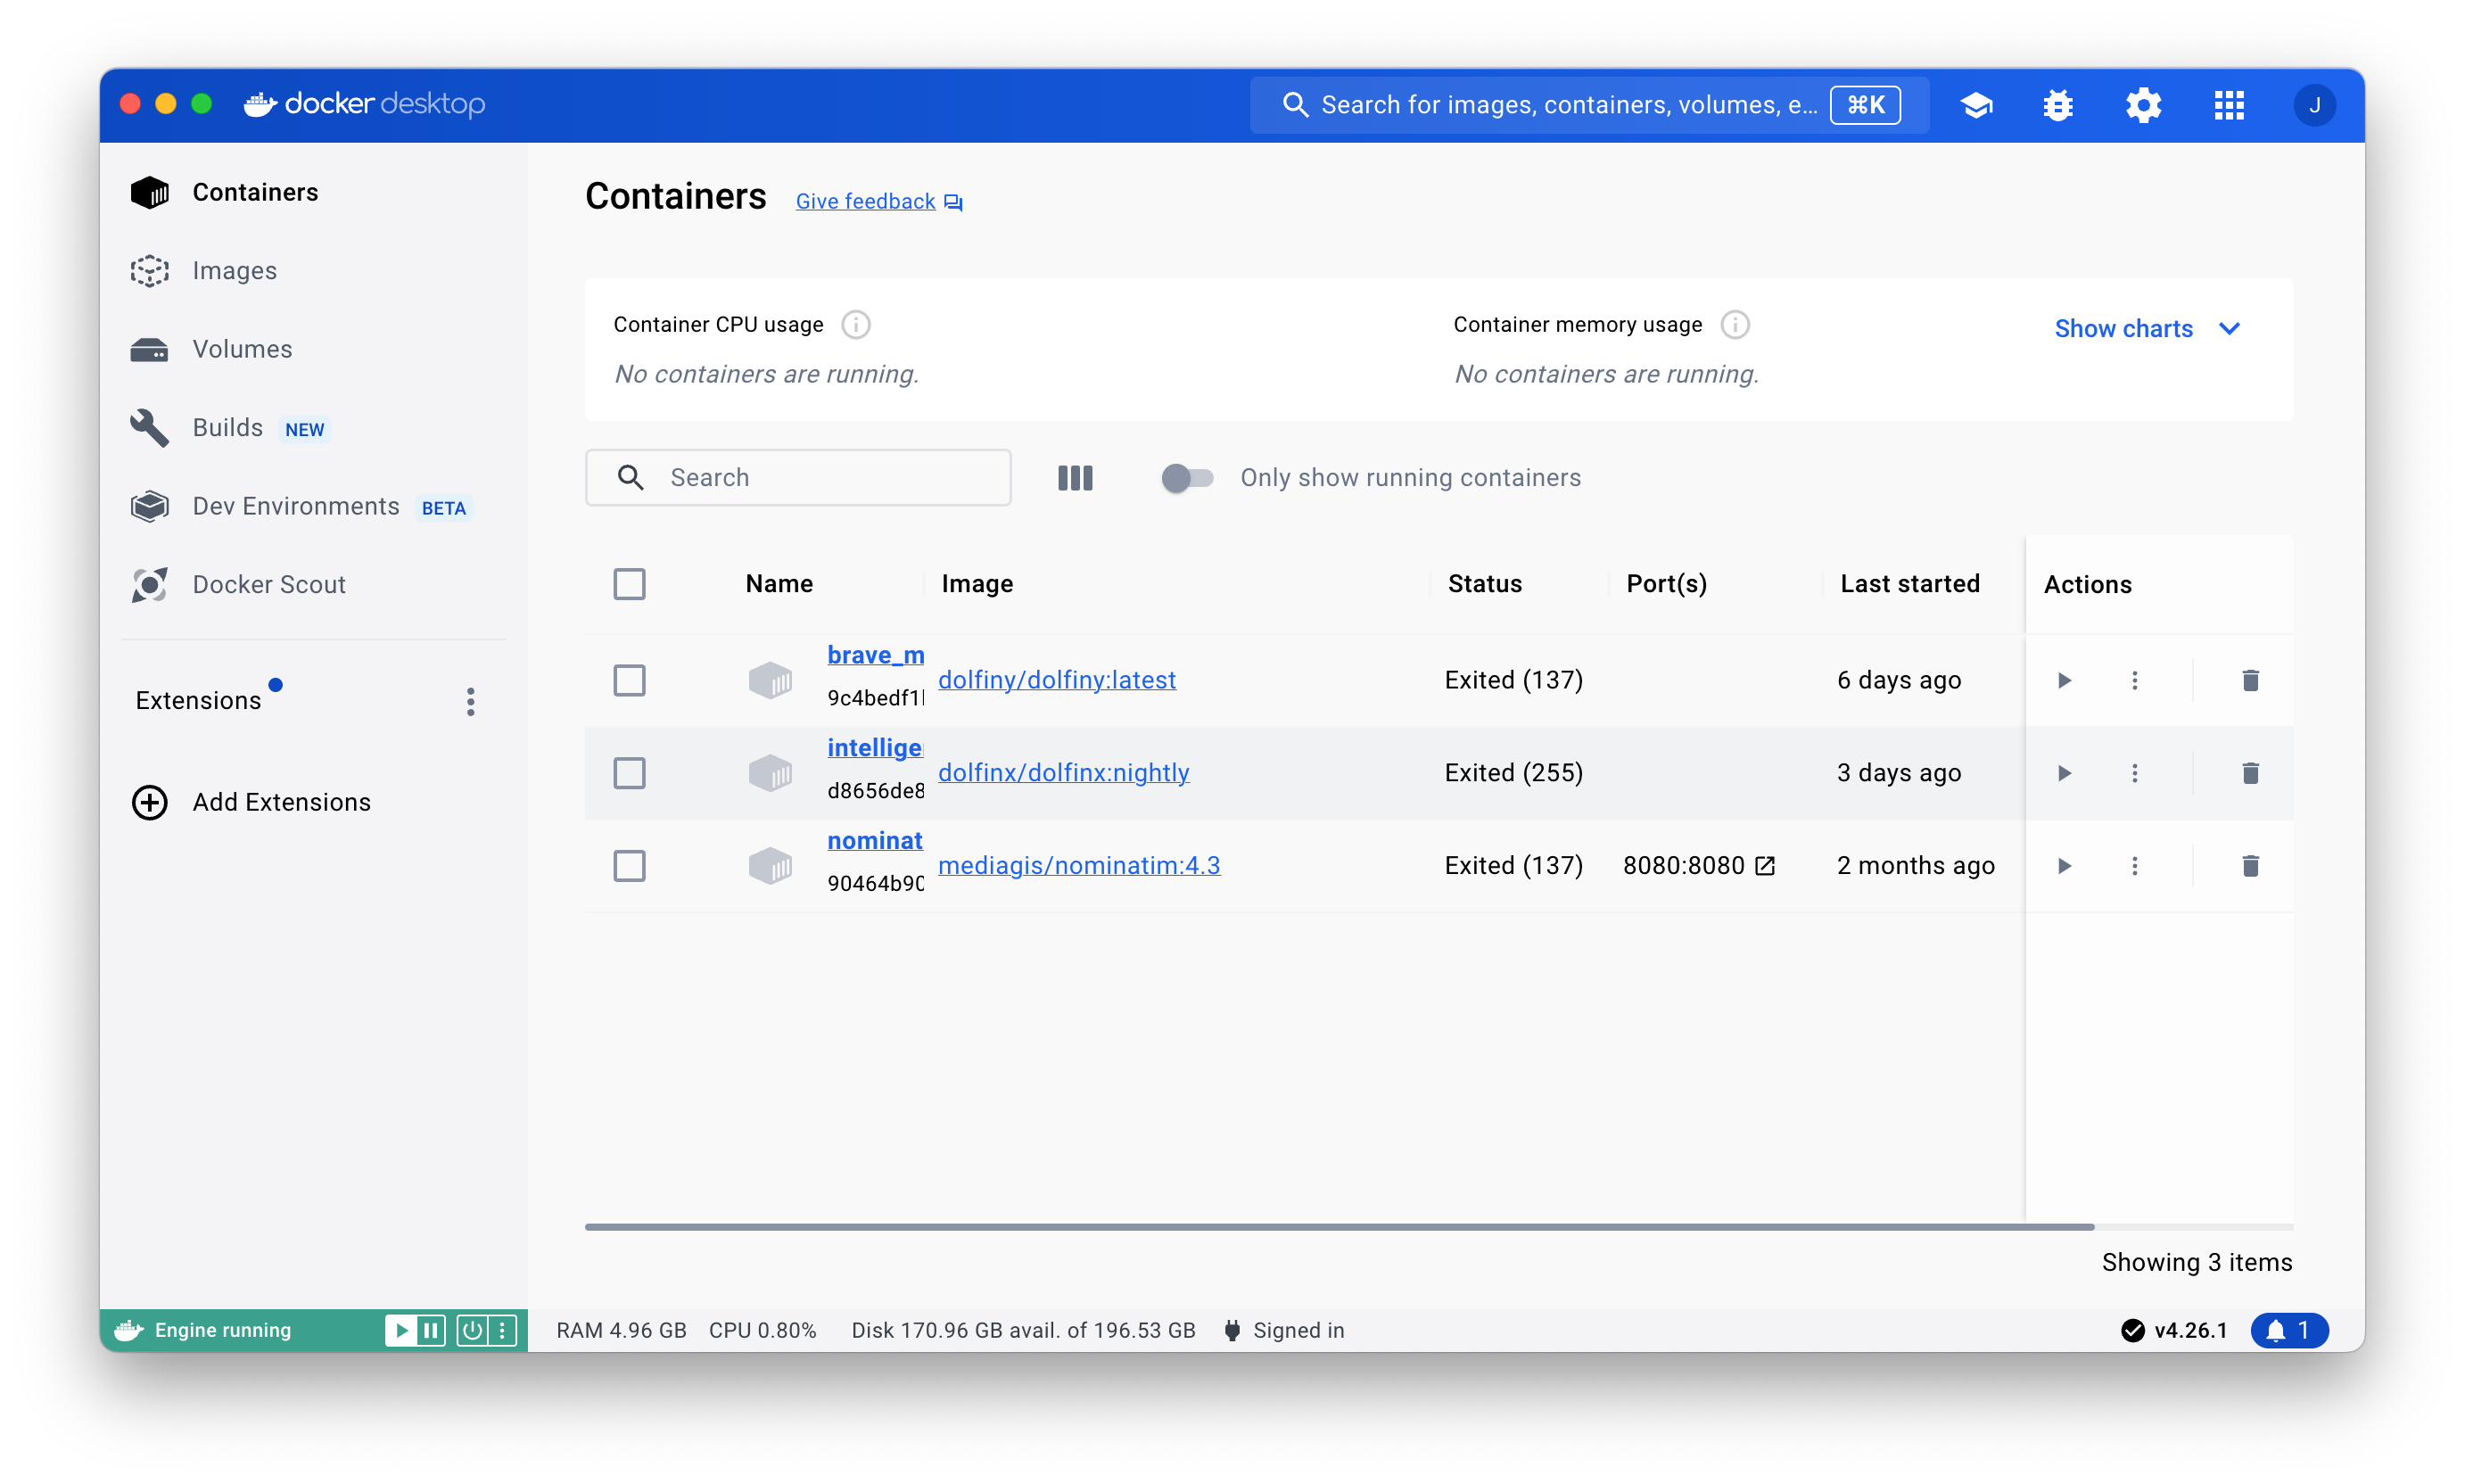
\includegraphics[width=0.7\textwidth]{DockerContainersTab.png}
  \caption{ The Docker Containers Tab}%
  \label{fig:docker_containers}%
\end{figure}

The docker containers tab has all of the container you have setup. Each container is essentially a different instance of a specific image. It is normally recommended that for every project you have a different seperate container made. Though those containers could use all the same image.

\subsection{Recommended Settings}

Because we will be running FEA software which will be want to use most of our computers resources, there are a few changes that should be made to optimize performance.


\begin{figure}[H]
  \centering
  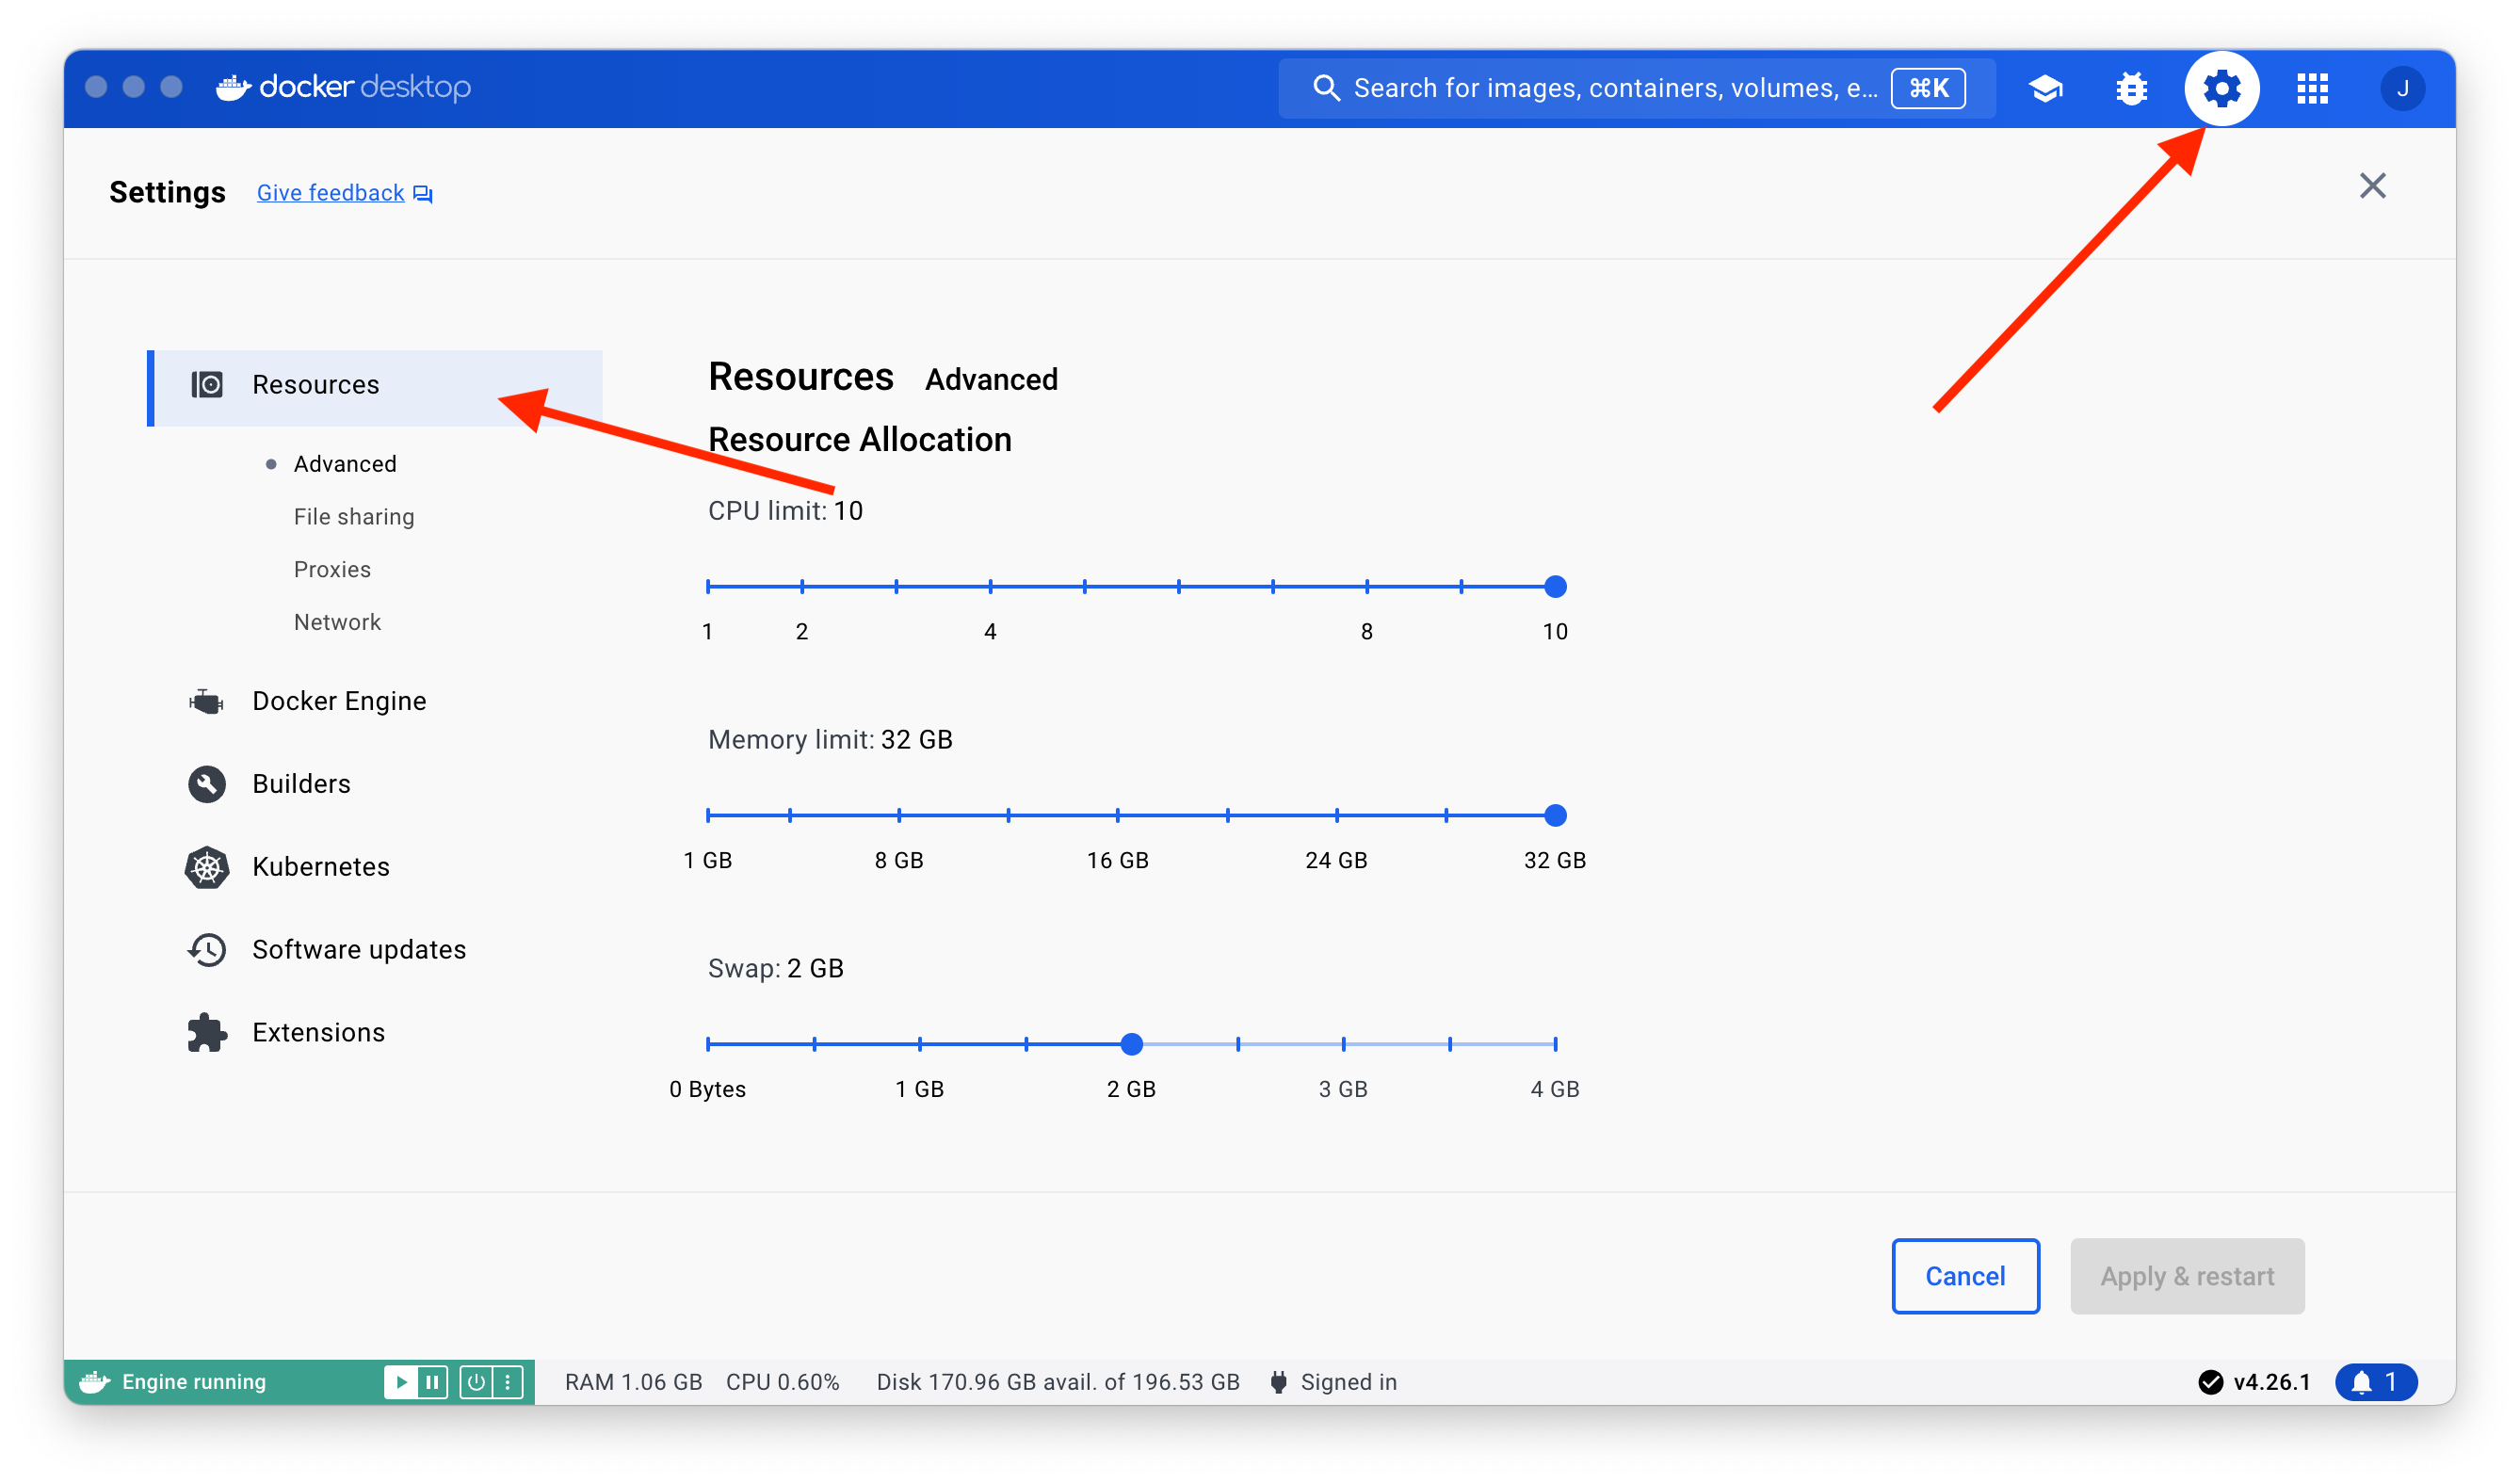
\includegraphics[width=0.7\textwidth]{DockerSetup.png}
  \caption{ The Docker Settings tab}%
  \label{fig:docker_settings}%
\end{figure}

We will be going to the docker settings tab, and then resources as seen in Figure \ref{fig:docker_settings}.
In here we will be maximizing the number of CPU's available and the memory limit.
\section{FEniCSx Container Setup}
In this section we will be setting up the FEniCSx image and container so that it runs properly.
We will also explain how to mount a folder in the volume so that it is shared between the host and docker container.

\subsection{Pulling the Image}
First we will need to pull the image from the docker hub. To do this we will need to open up the terminal.

On a mac we can press ctrl+space and then type in terminal to open it up.
\begin{figure}[H]
  \centering
  \includegraphics[width=0.7\textwidth]{TerminalOpening.png}
  \caption{ The Docker Settings tab}%
  \label{fig:Terminal_open}%
\end{figure}

Once the terminal is open we will need to type in the following command:

\begin{lstlisting}[language=bash, caption=Docker Pull Command]
  > docker pull jorgenin/dolfinx-2.077:v0.8
\end{lstlisting}

Which will download the image and prepare it on your computer.

Figure \ref{fig:Terminal_pull_done} shows what the output will be.
\begin{figure}[H]
  \centering
  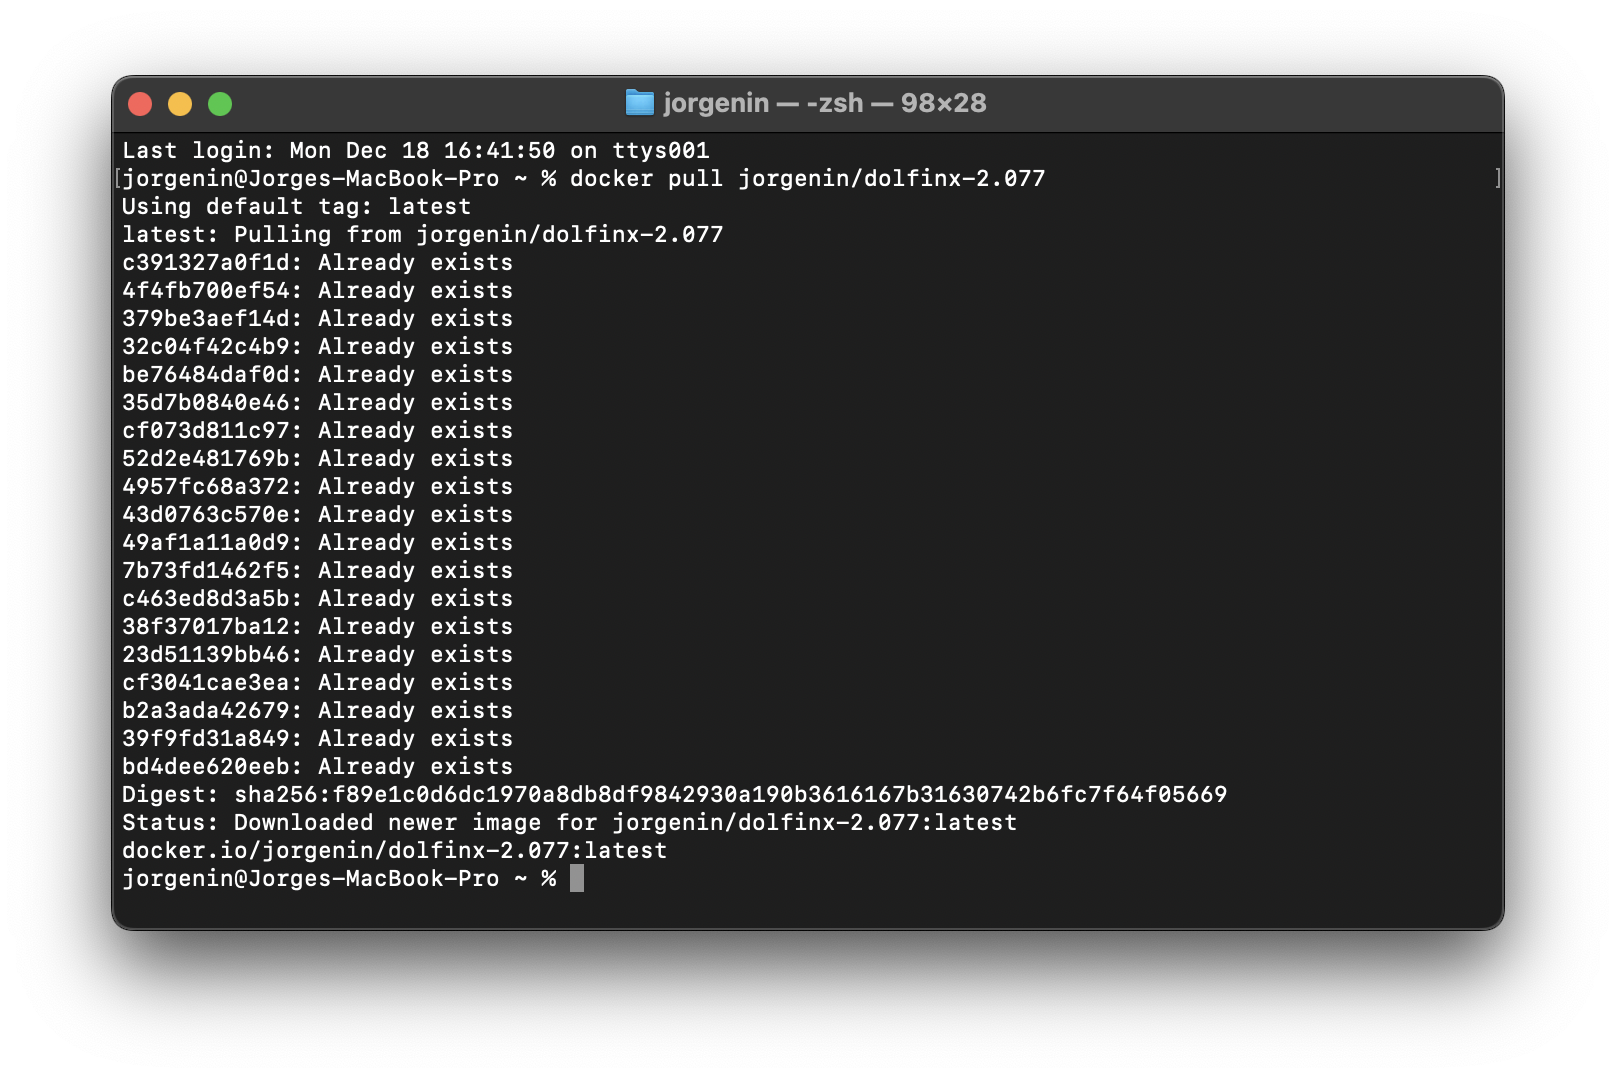
\includegraphics[width=0.7\textwidth]{TerminalImage_pull.png}
  \caption{Output from the terminal}%
  \label{fig:Terminal_pull_done}%
\end{figure}

\subsection{Creating the Container}
Now that we have the image downloaded we can create a container from it.
\begin{lstlisting}[language=bash, caption=Docker Pull Command]
  > docker run -it jorgenin/dolfinx-2.077:v0.8
\end{lstlisting}

This command will create the container and run it in interactive mode.
Explaining it in more detail:

\clist{docker run} will create a container from the image we specify. \clist{-it} will run the container in interactive mode. \clist{jorgenin/dolfinx-2.077} is the image we want to use.
\clist{:v0.8} is the tag. We could also use for example \clist{:latest} to get the latest version of the image or \clist{:v0.7} to get the 0.7 version of the image.


Upon executing this command we will be inside of the container and activly running the image.

If we look at the docker desktop application we will see that a container has been created as showing in Figure \ref{fig:docker_container_created}

\begin{figure}[H]
  \centering
  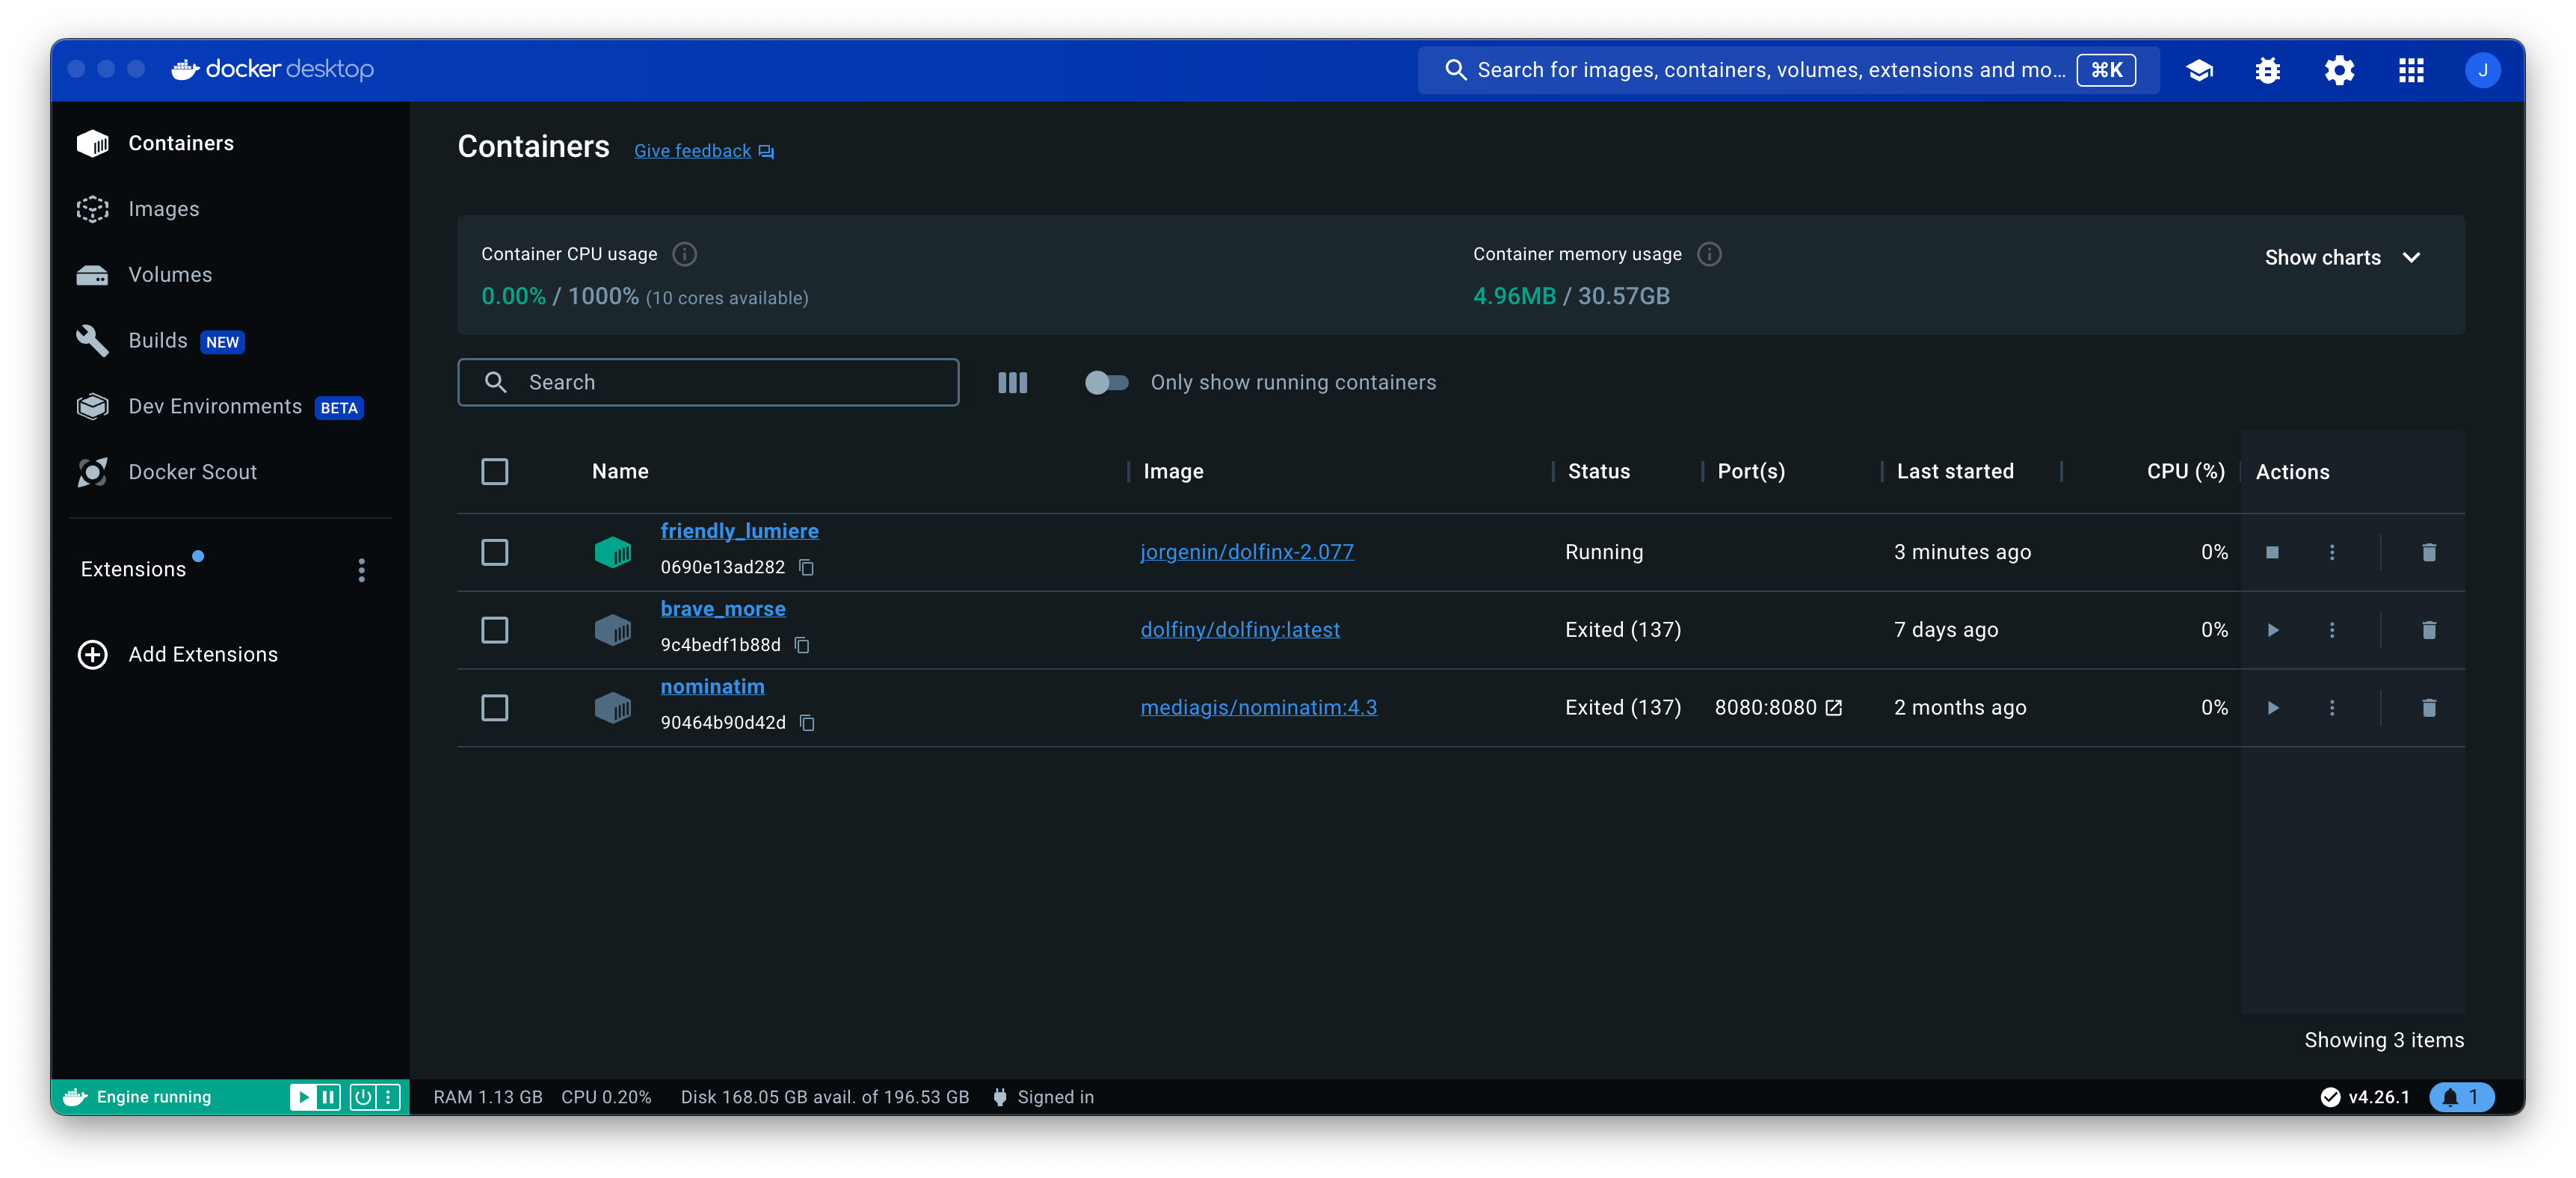
\includegraphics[width=0.7\textwidth]{DockerContainerRunning.png}
  \caption{And image from the docker desktop application showing the docker container running.}%
  \label{fig:docker_container_created}%
\end{figure}



We can exit the container by typing \clist{exit}.

\subsection{Connecting to a Container that was created}

If we run the past section multiple times we'll create multiple independent containers. As such when developing we'll normally want to just connect to a conatiner that has already been created.

We can do that through either the terminal or the docker desktop application.
\subsubsection{Connecting through a terminal}

We can run the following command to run the container interactivly (connecitng to the container immediatly)
\begin{lstlisting}[language=bash]
  > docker start -i "container name":"container tag"
\end{lstlisting}

If we look at Figure \ref{fig:docker_container_created} we can see the container we created is called \clist{friendly_lumiere}.
So in our case the command would be:
\begin{lstlisting}[language=bash]
  > docker start -i friendly_lumiere
\end{lstlisting}

If we just want the command to run the background we can just omit the \clist{-i}. This has the advantage that if we close the terminal the container will continue to run.

\begin{lstlisting}[language=bash]
  > docker start friendly_lumiere
\end{lstlisting}

We could then connect to it at any point by running:
\begin{lstlisting}[language=bash]
  > docker attach friendly_lumiere
\end{lstlisting}

\subsubsection{Connecting through the Docker Desktop Application}
The docker desktop application is more intuitive (though it does have limitations).
To start a container we can just click the play button next to the container we want to run as shown in Figure \ref{fig:docker_how_to_run}.
\begin{figure}[H]
  \centering
  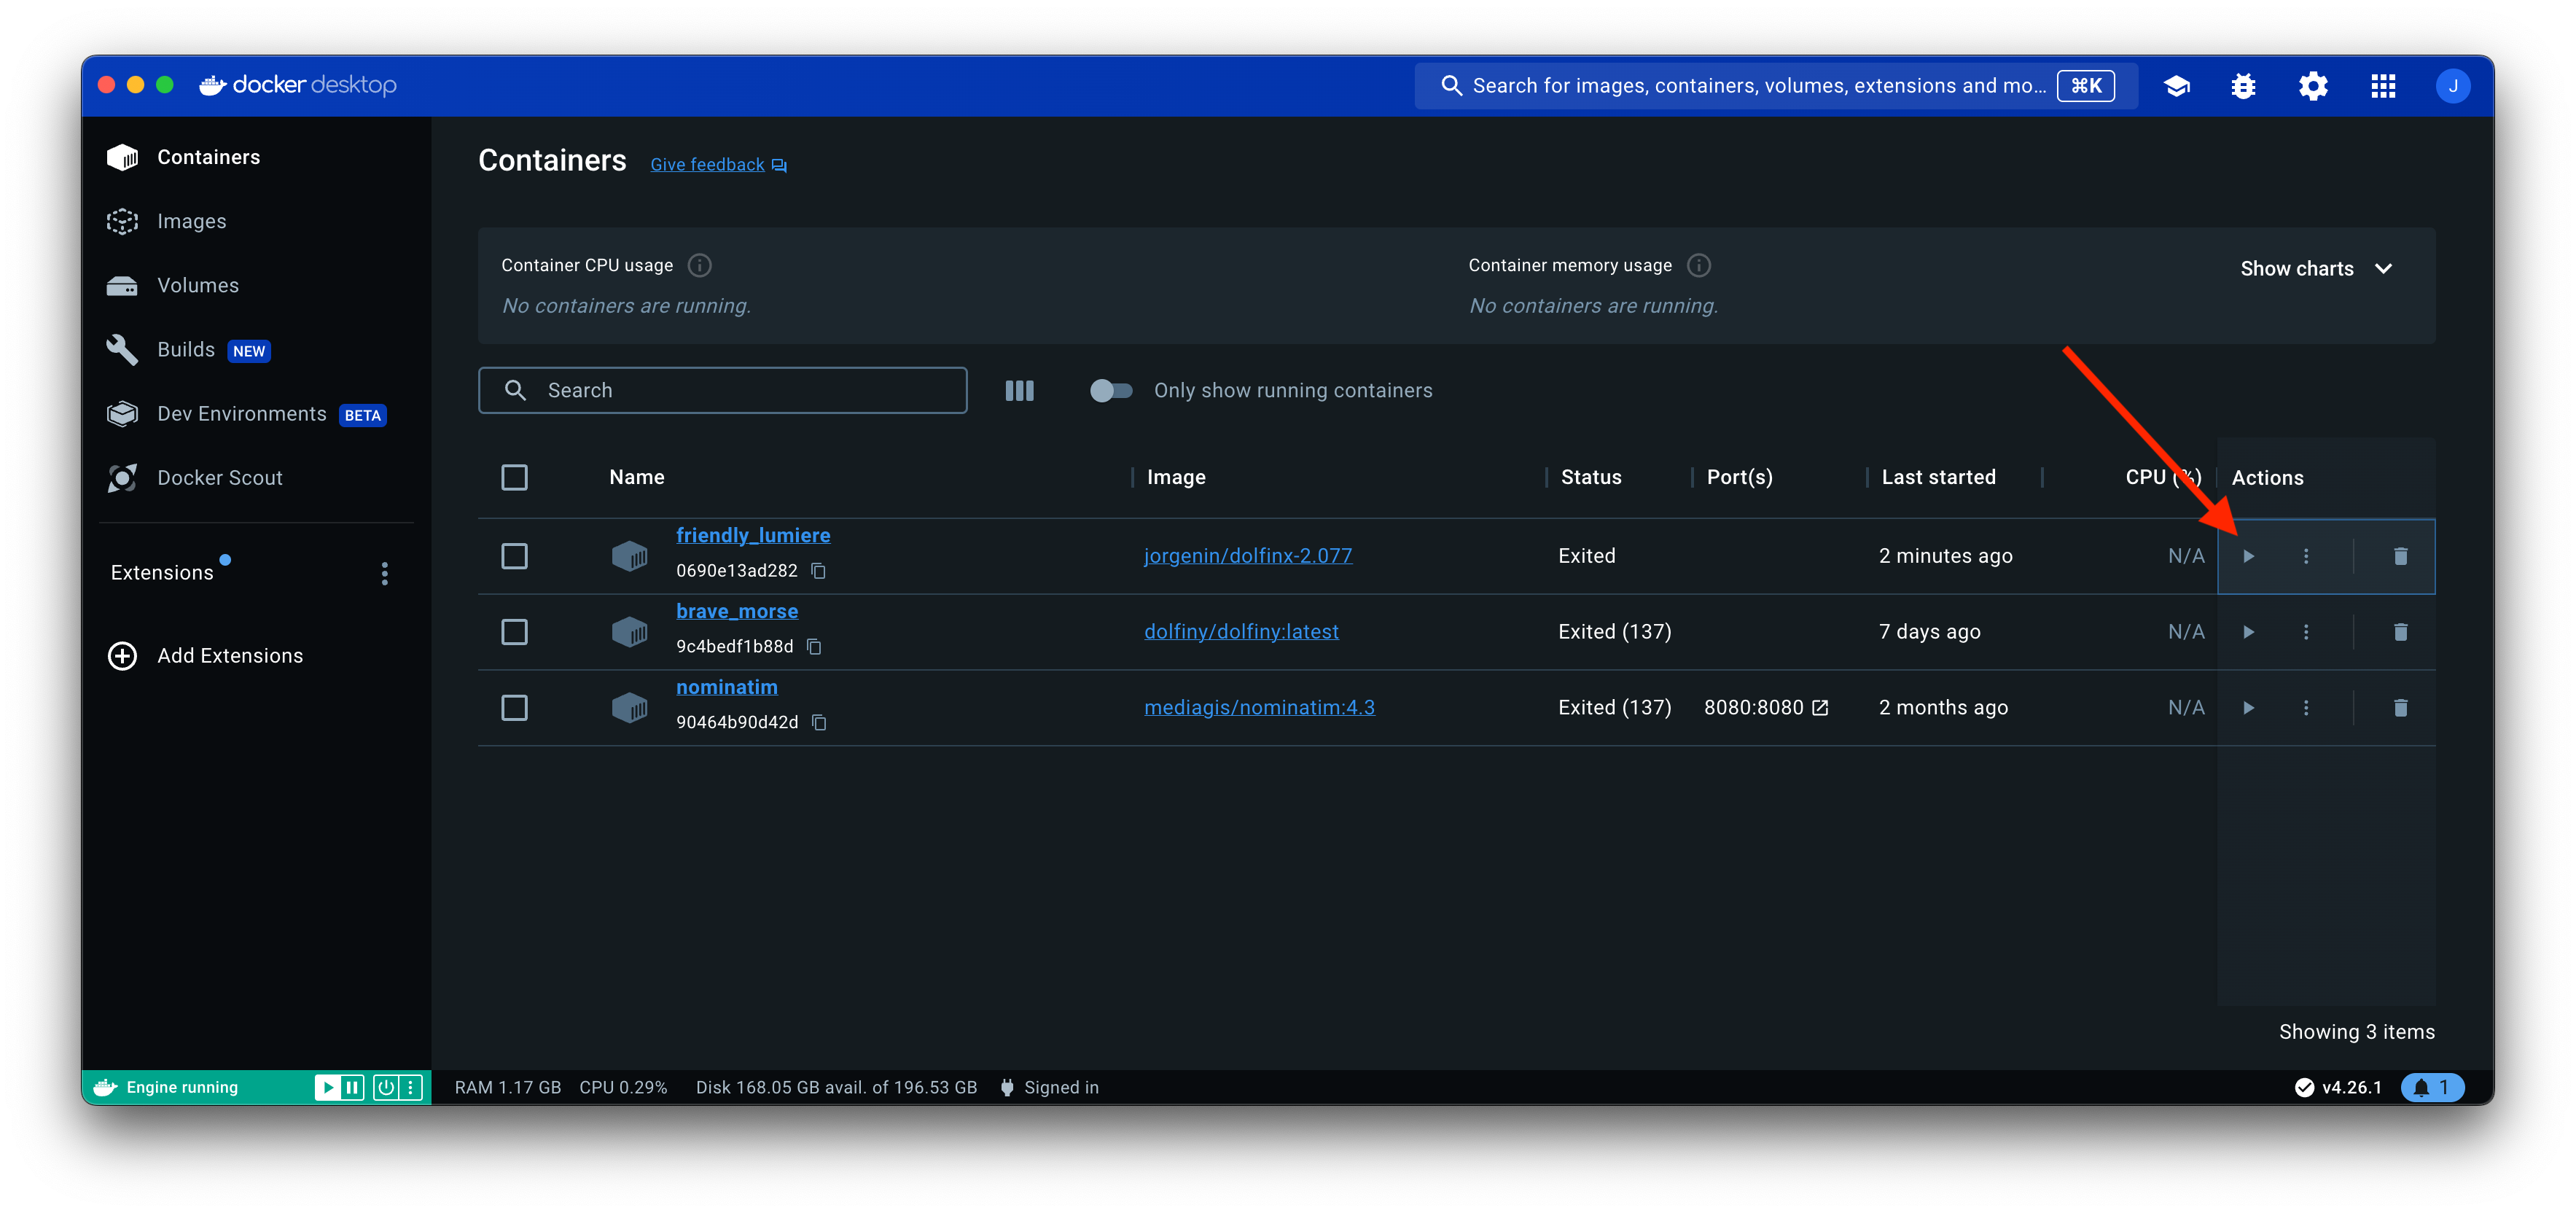
\includegraphics[width=0.7\textwidth]{DockerRUNHOW.png}
  \caption{How to start a container in docker desktop}%
  \label{fig:docker_how_to_run}%
\end{figure}


If we want to attach to a running container we can then click on the three dots and then click on \clist{Open In Terminal} as seen in \ref{fig:docker_how_to_connect}

\begin{figure}[H]
  \centering
  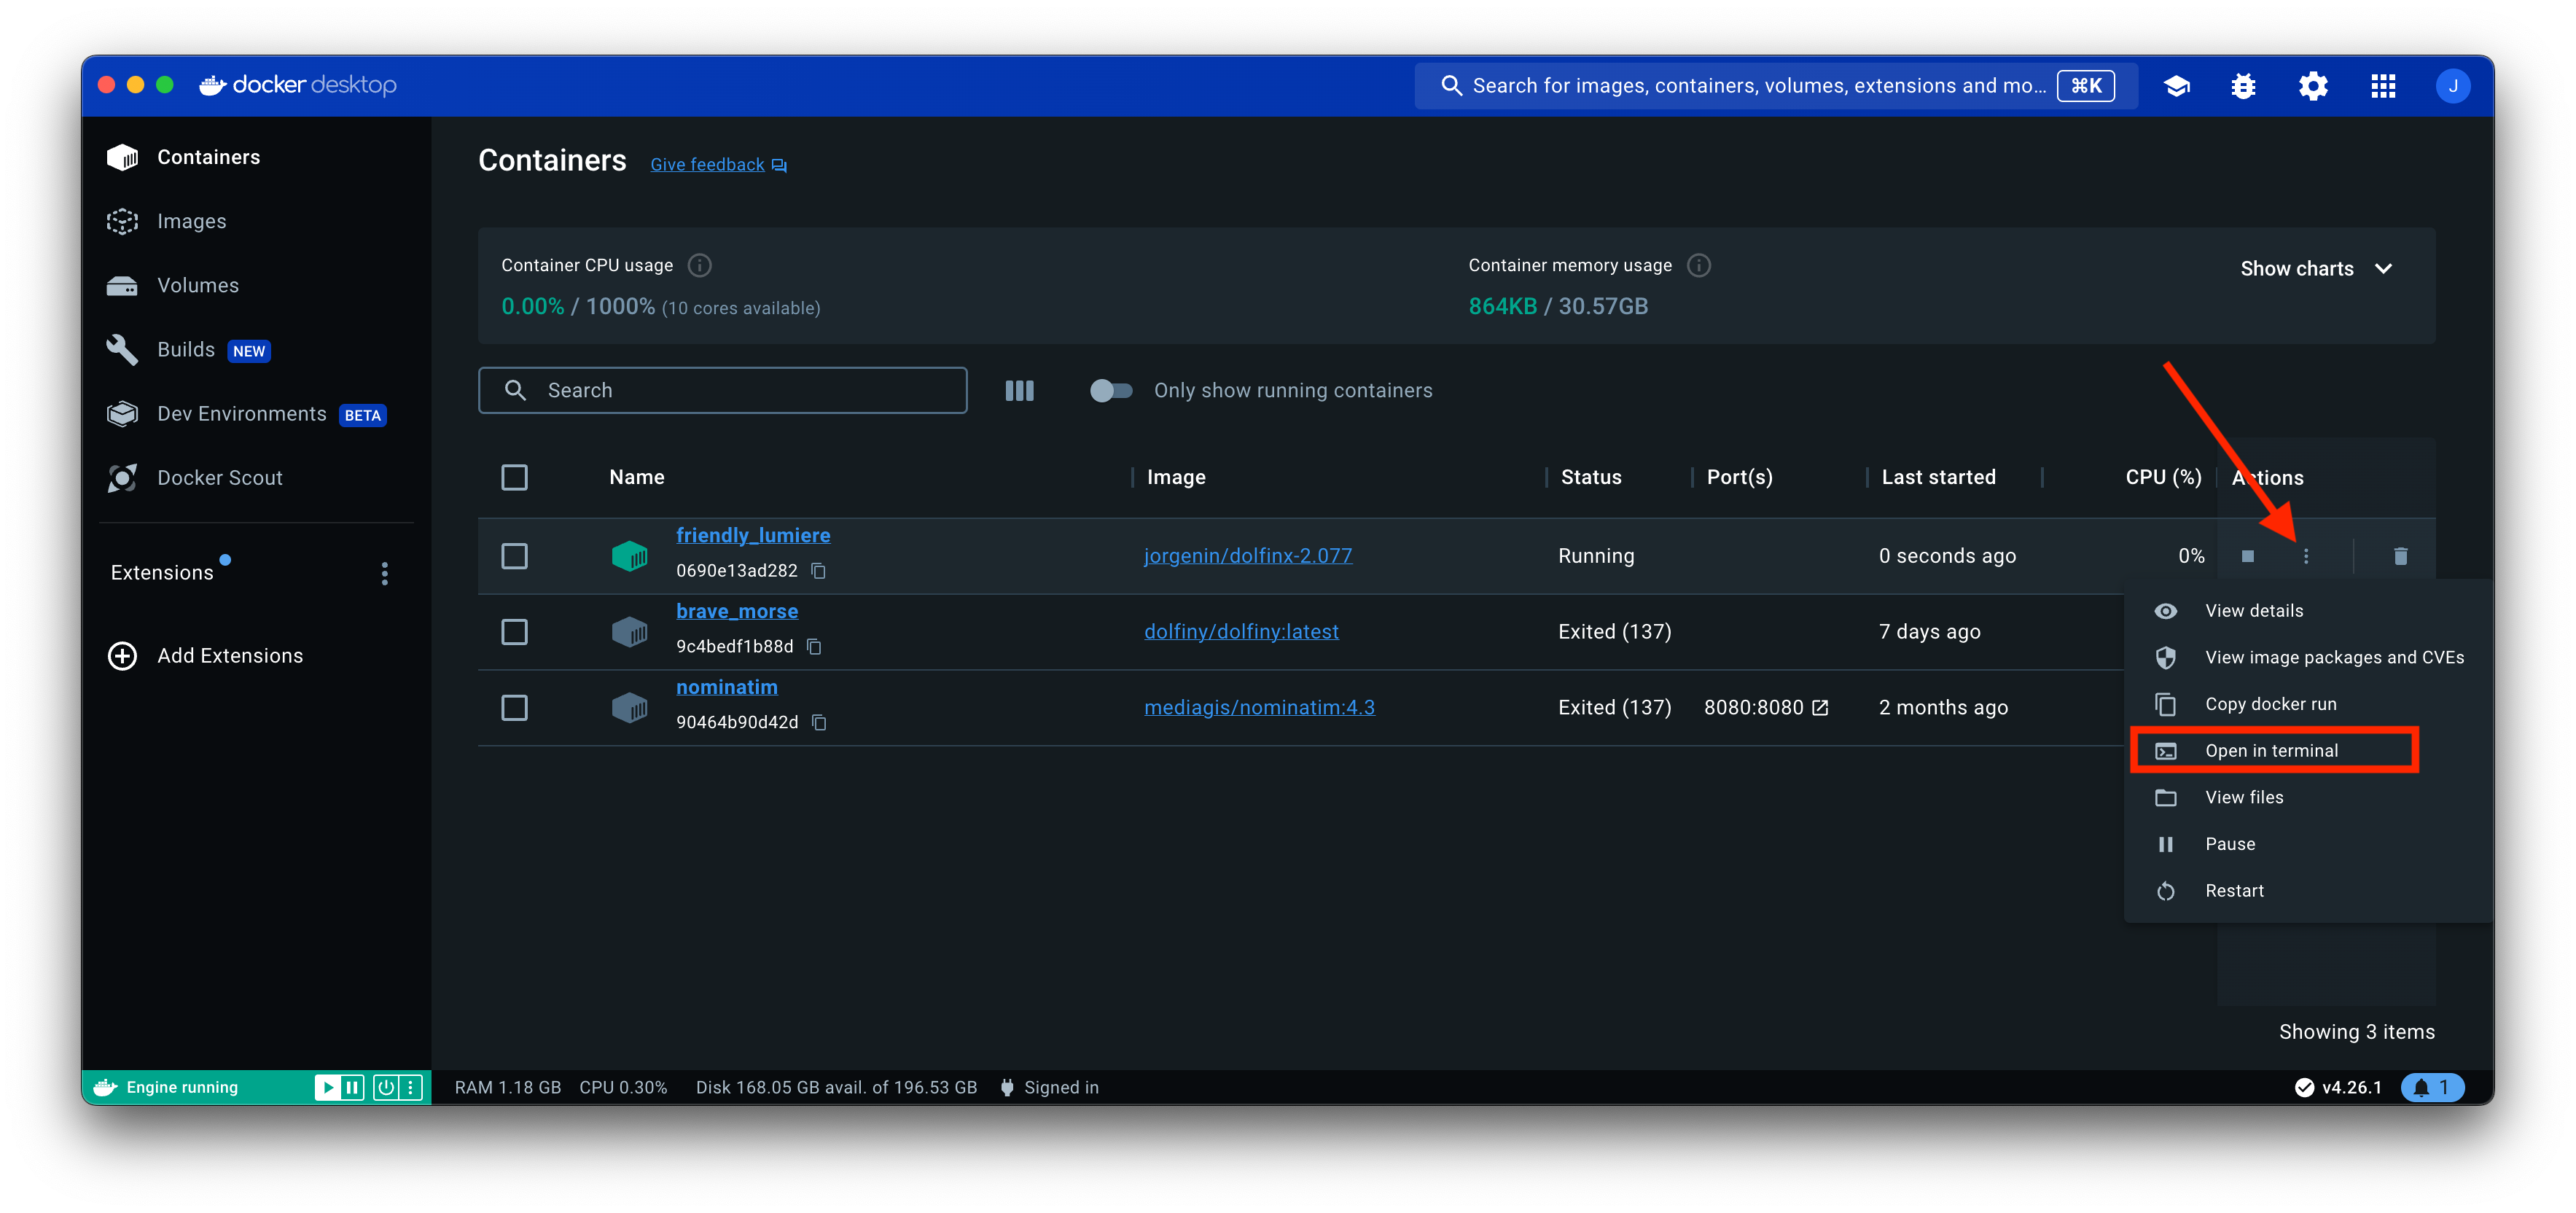
\includegraphics[width=0.7\textwidth]{DockerDesktop_CLI.png}
  \caption{How to Connect to DockerTerminal}%
  \label{fig:docker_how_to_connect}%
\end{figure}

\subsection{Sharing A Folder}
To share (or mount) a folder between the host and the container we will need to use the \clist{-v} flag when creating the container.

\begin{lstlisting}[language=bash]
  > docker run -it -v "folder path":"container folder path" jorgenin/dolfinx-2.077:v0.8
\end{lstlisting}

For example if we wanted to share the folder \clist{/users/jorgenin/Documents/2.077-FEniCSx-Finite-Elasticity} with the container we would run the following command:

\begin{lstlisting}[language=bash]
  > docker run -it -v /users/jorgenin/Documents/2.077-FEniCSx-Finite-Elasticity:/home/project jorgenin/dolfinx-2.077:v0.8
\end{lstlisting}

Now any files that are in the folder on the OS will be shown to the container and viceversa.

\section{VSCode}

VS Code will be our main development software we will be using. It's very flexible and supports a multitude of programming languages.
To install it download it from Microsoft here \href{https://code.visualstudio.com/download}{VSCode Download} and install it.
The process is very similar to installing docker.

\subsection{VSCode Extensions}

The main idea behind vscode is that can be easily customized to any usecase through the liberal use of extensions.

To simplify the process we have created a custom extension pack with most everything you'll need to get started.
To download and install it click on the following link: \href{https://marketplace.visualstudio.com/items?itemName=2077MIT.2-077-fenicsx-extension-pack}{VSCode FEniCSx Extension Pack} and click on install.

Another way to do so (and to install your own extensions) is to click on the extensions tab on the left side of the screen and then search for the extension you want to install.
You can see the process in Figure \ref{fig:vscode_extension_install}.

\begin{figure}[H]
  \centering
  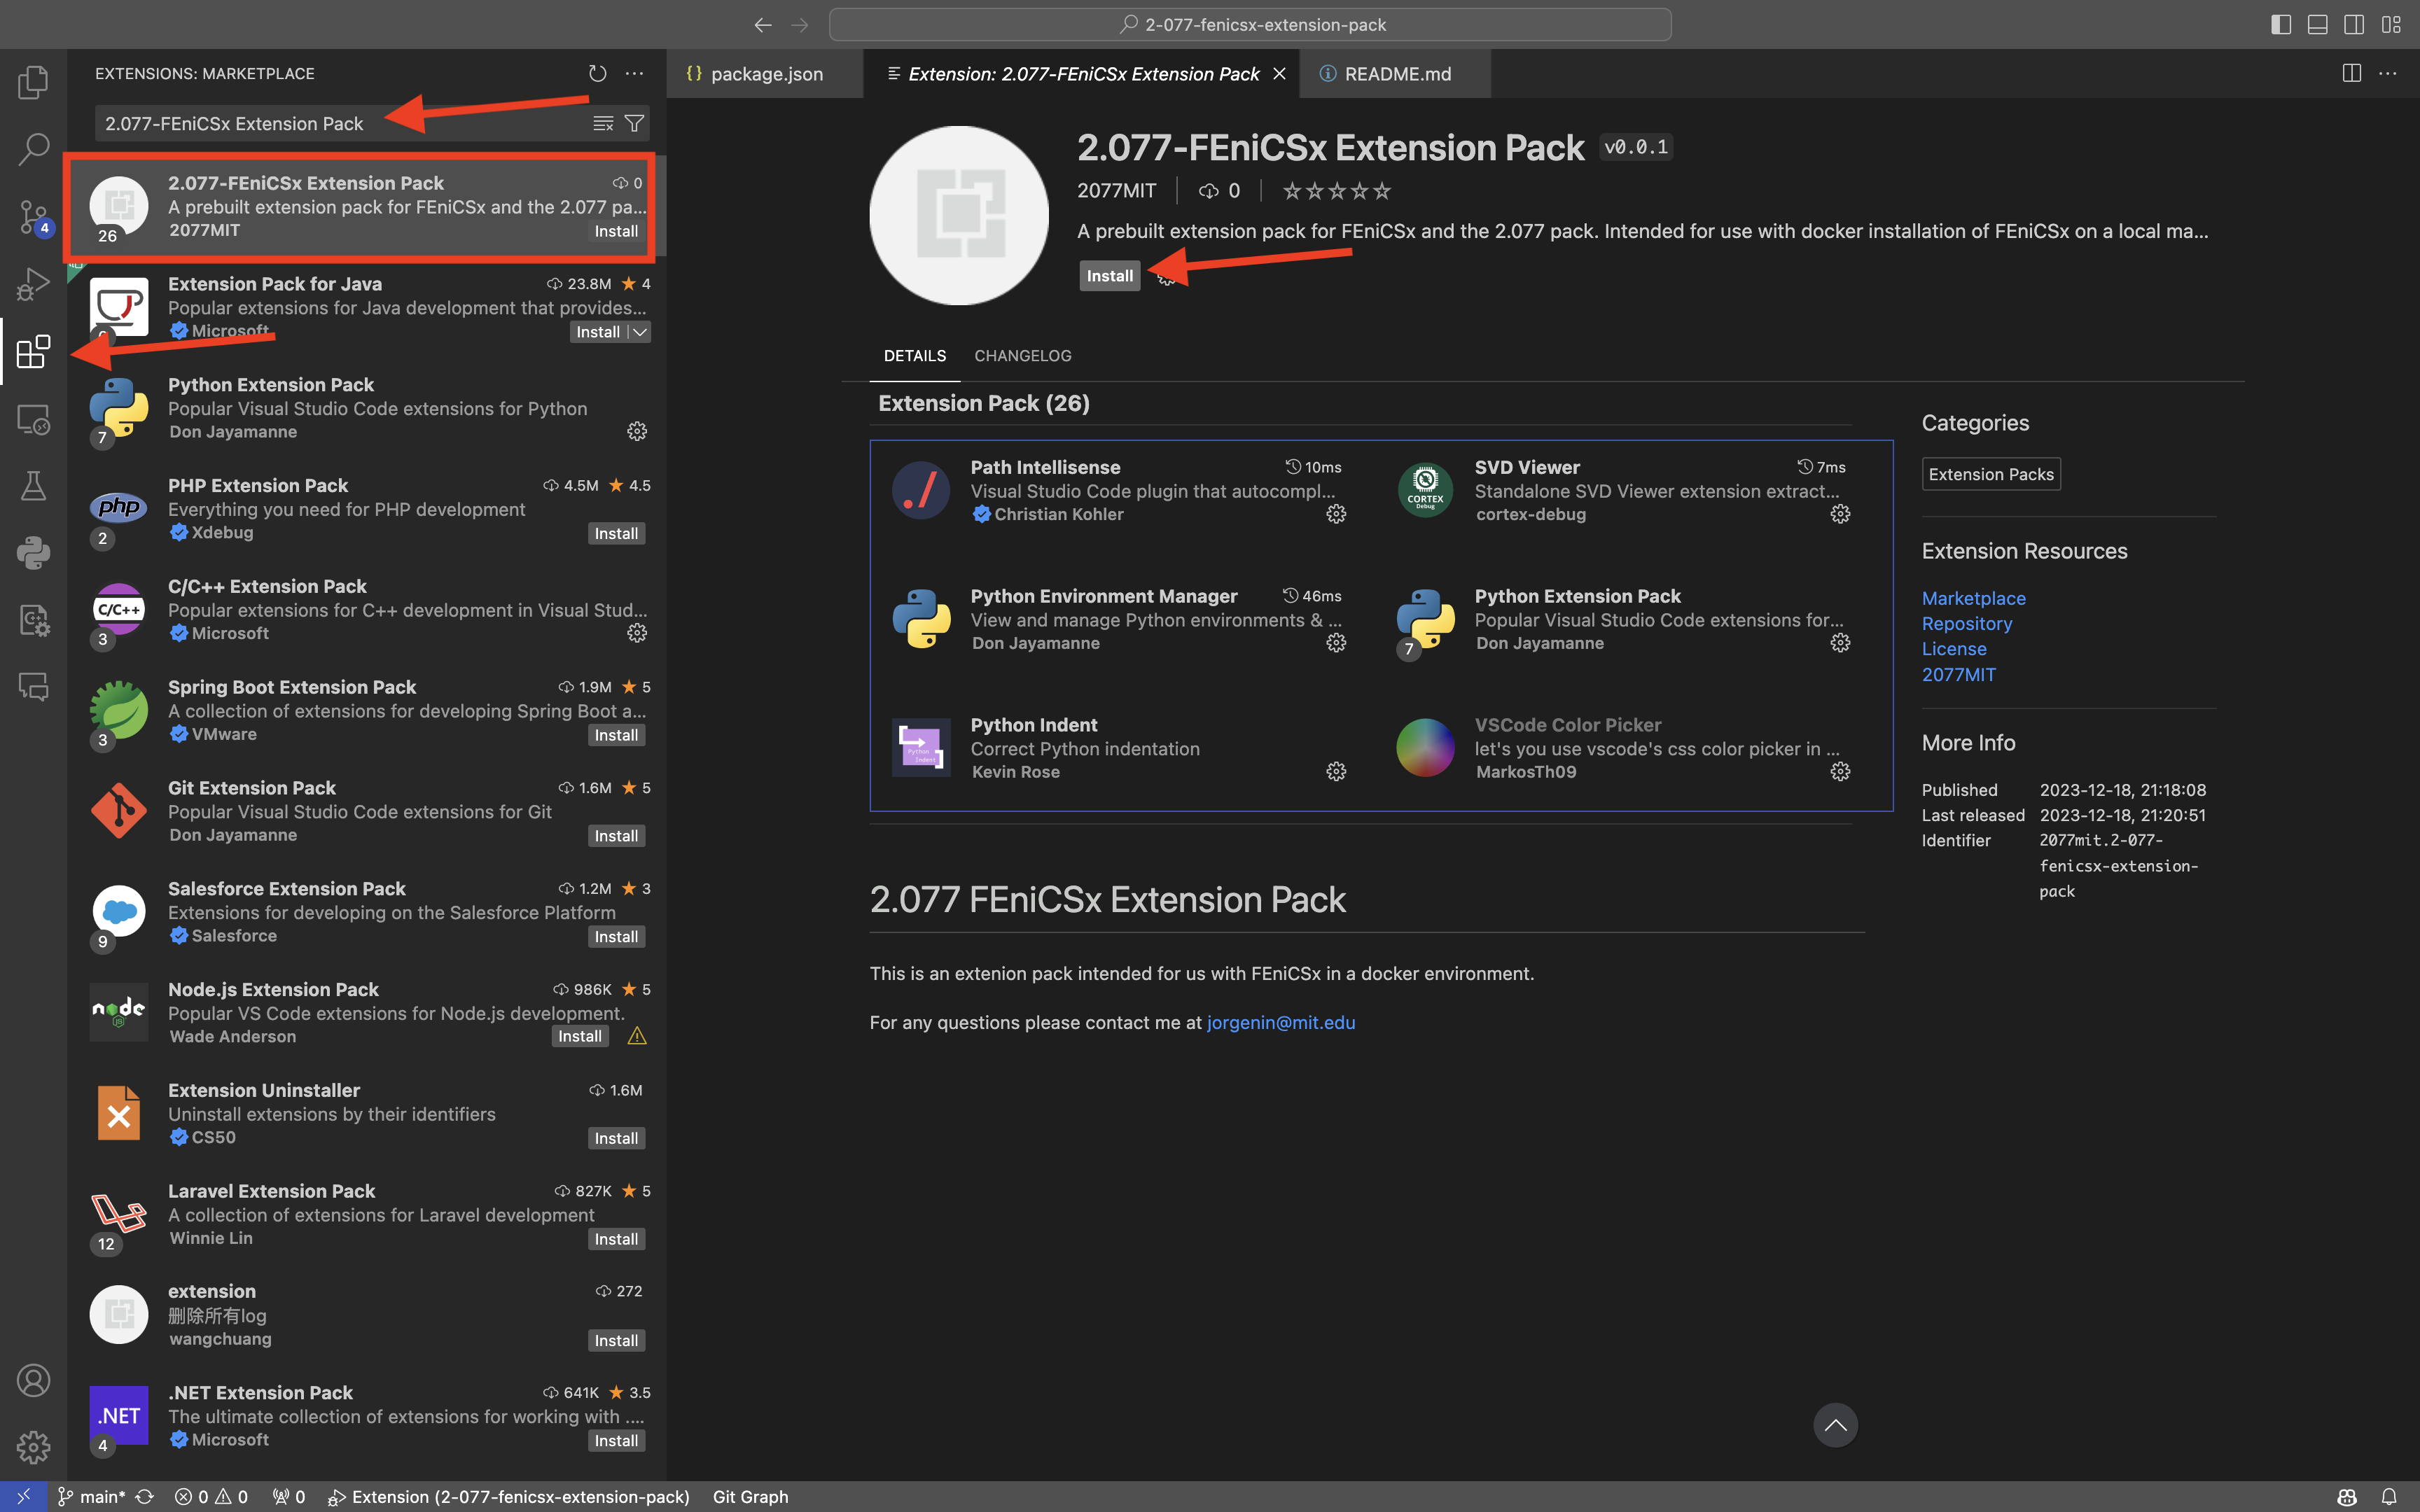
\includegraphics[width=0.7\textwidth]{VSCodeExtensionInstall.png}
  \caption{How to install extensions in vscode}%
  \label{fig:vscode_extension_install}%
\end{figure}


\section{Running Example Program}

With the previous steps completed we should now be prepared to actually run a real example.
Here I will walk through step by step from initializing an image to finally running it, and connecting to it through VS Code.

Through this section we will assume you have done all of the basic setup steps previous mentioned.

\subsection{Pulling the Image}
To pull an image we will open up a terminal and run the command:
\begin{lstlisting}[language=bash, caption=Docker Pull Command]
  > docker pull jorgenin/dolfinx-2.077:v0.8
\end{lstlisting}

We will see the following output from the terminal:
\begin{figure}[H]
  \centering
  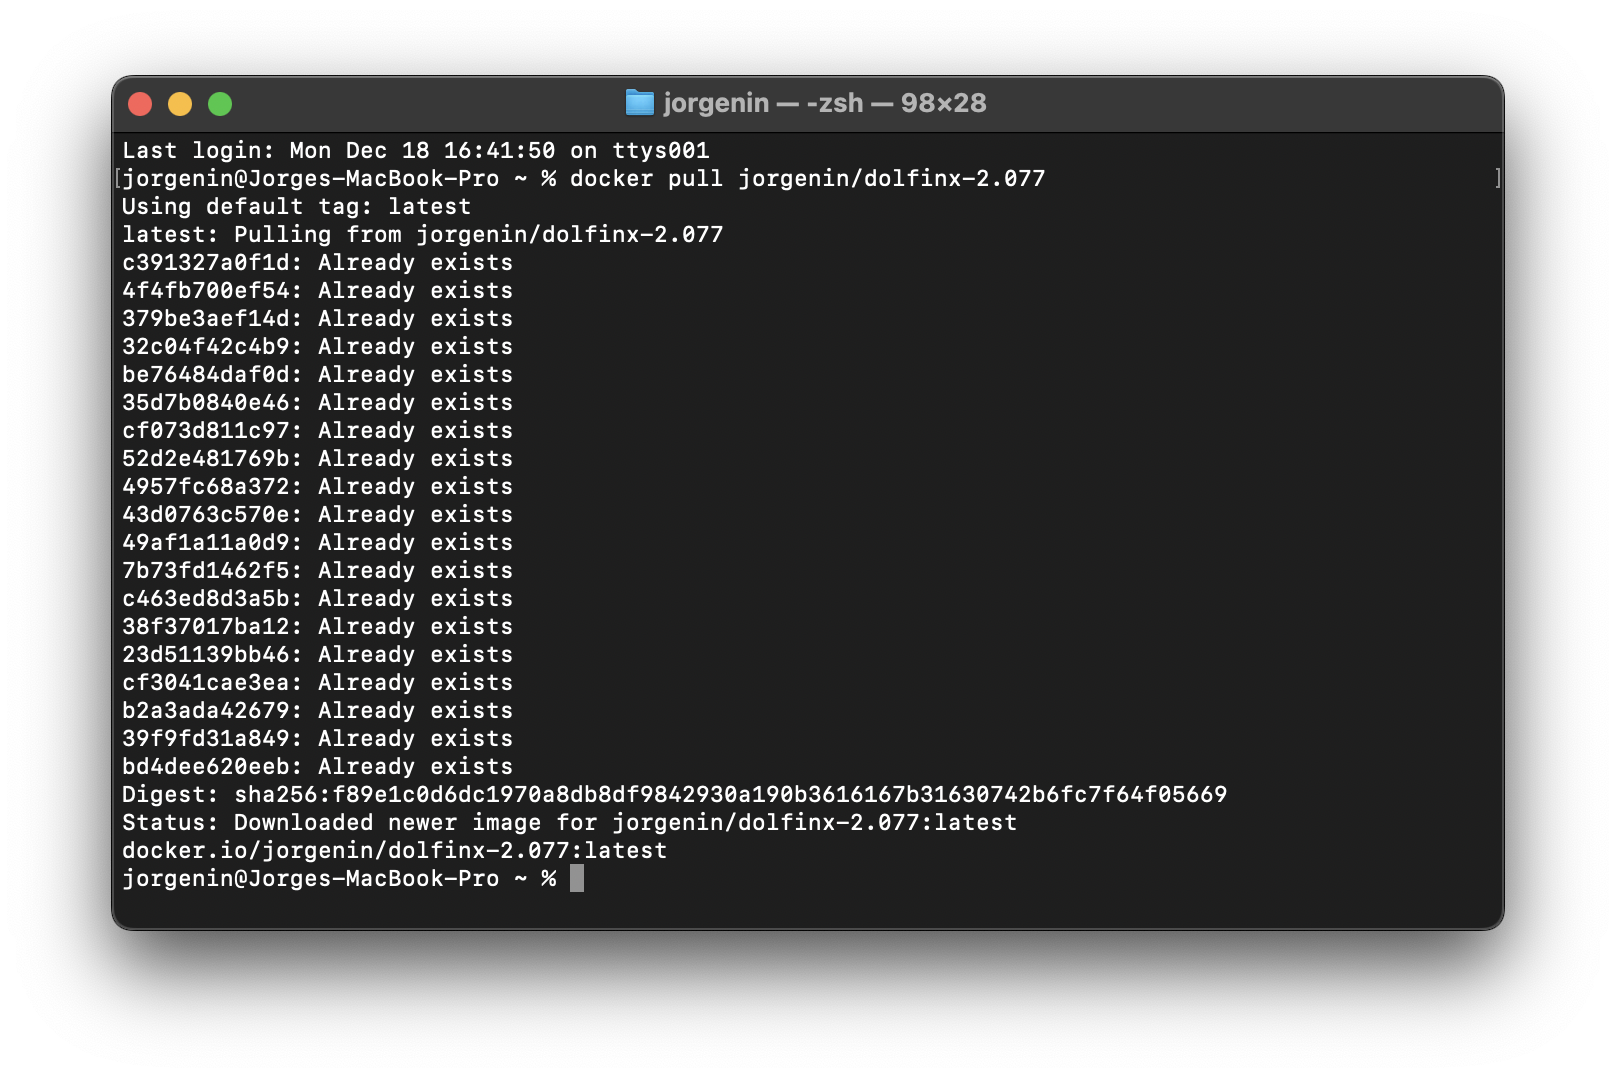
\includegraphics[width=0.7\textwidth]{TerminalImage_pull.png}
  \caption{Output from the terminal}%
  \label{fig:Terminal_pull_done_2}%
\end{figure}

\subsection{Creating the Container}
Here we will be creating the container and mounting a local folder to it from where we will be running all of the results.
We will be mounting a folder \clist{/Users/jorgenin/Desktop/fenicsx-tutorial} to the opening folder of the docker instance \clist{/home/project}.

The command is:
\begin{lstlisting}[language=bash, caption=Docker Pull Command]
> docker run -it -v /Users/jorgenin/Desktop/fenicsx-tutorial:/home/project jorgenin/dolfinx-2.077:v0.8
\end{lstlisting}

We can see the results in Figure \ref{fig:Terminal_mount_image}.
\begin{figure}[H]
  \centering
  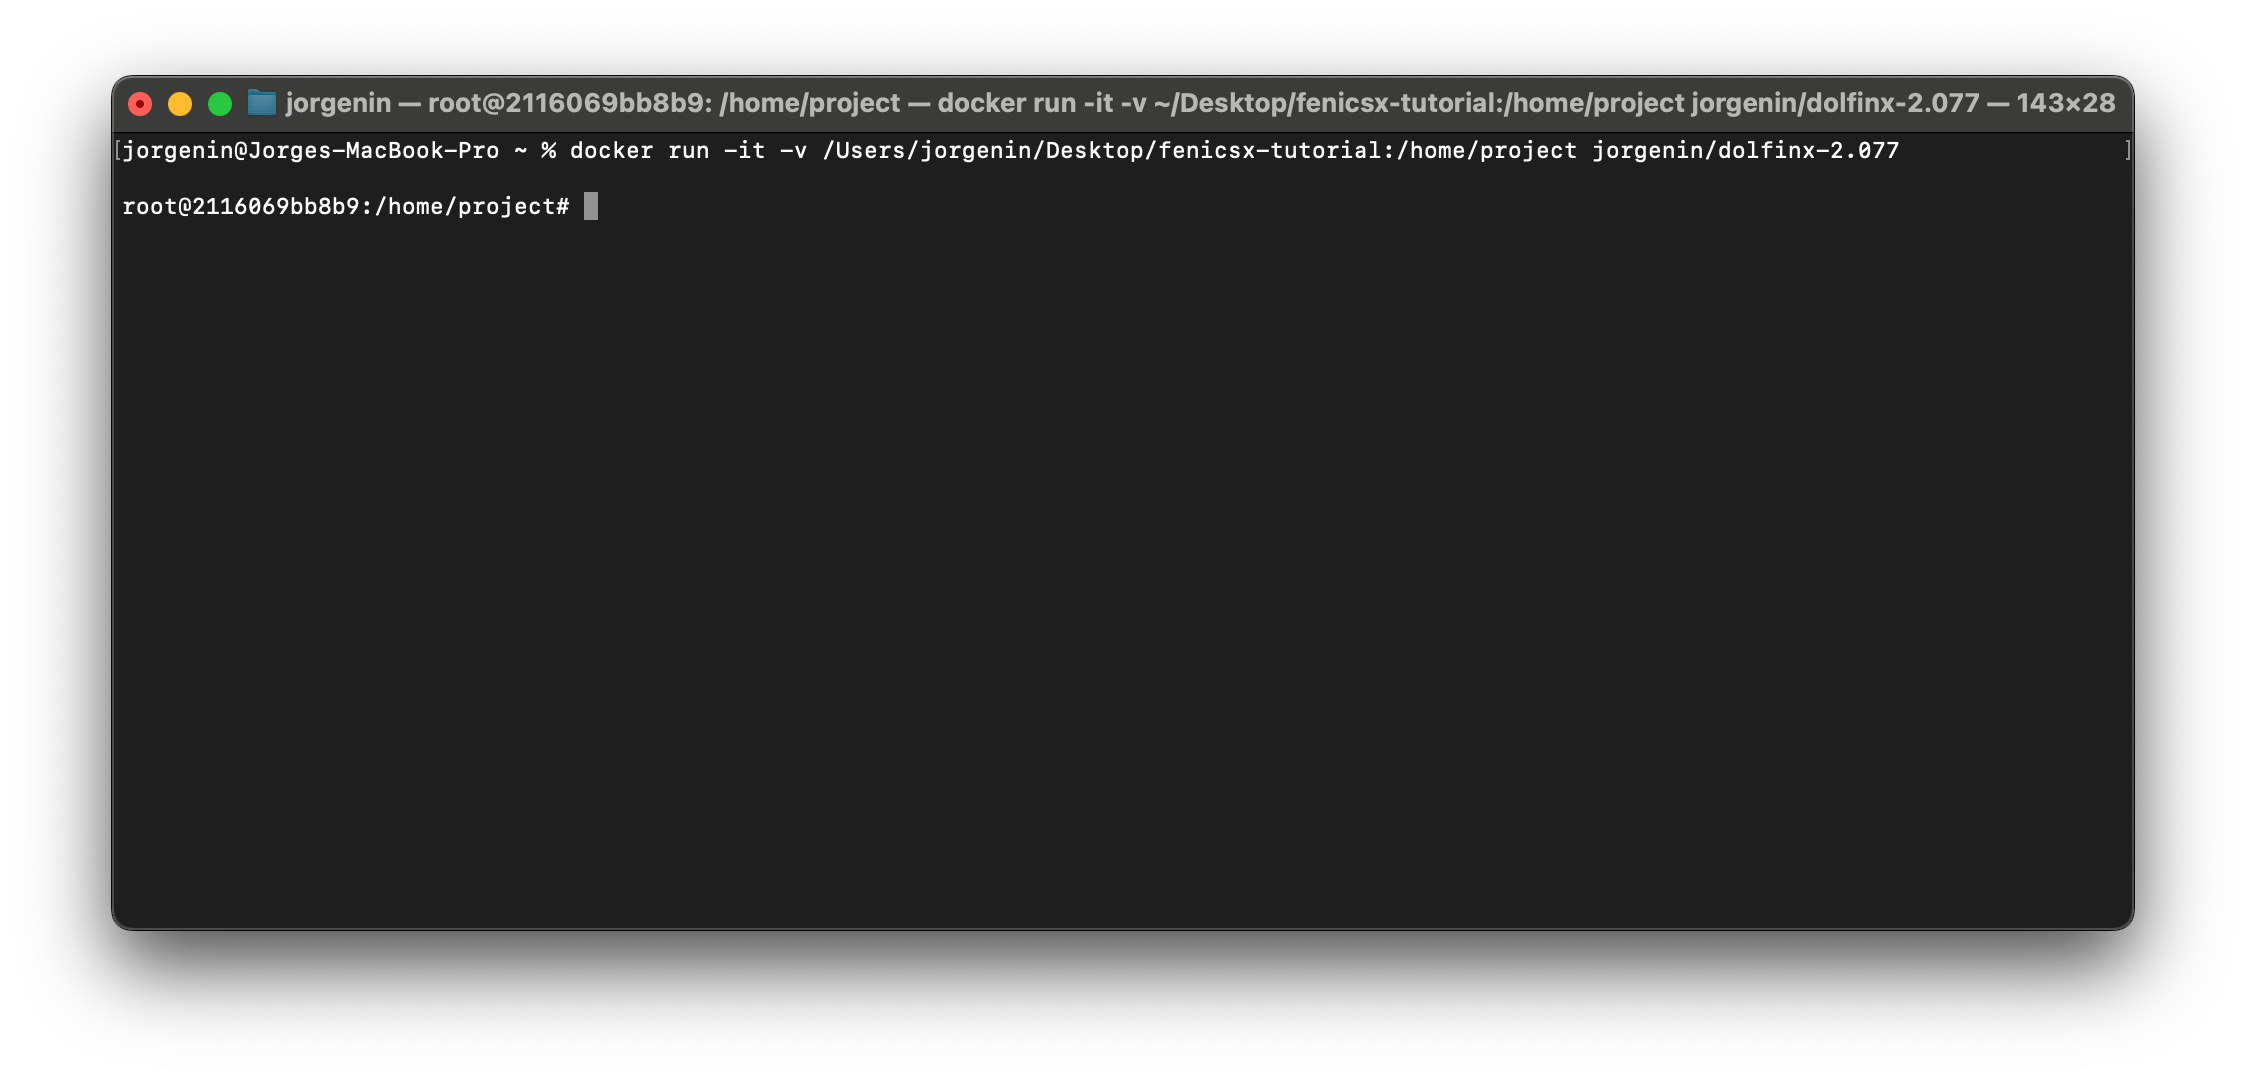
\includegraphics[width=0.7\textwidth]{Container-Monted-Folder.png}
  \caption{Output from the terminal after mounting image}%
  \label{fig:Terminal_mount_image}%
\end{figure}

\subsection{Connecting to the Container through VSCode}

We now launch vscode and connect to the container we just created.
We can go to the docker extension, find the container we just launched right click on it and then click attach \clist{Visual Studio Code}.
\begin{figure}[H]
  \centering
  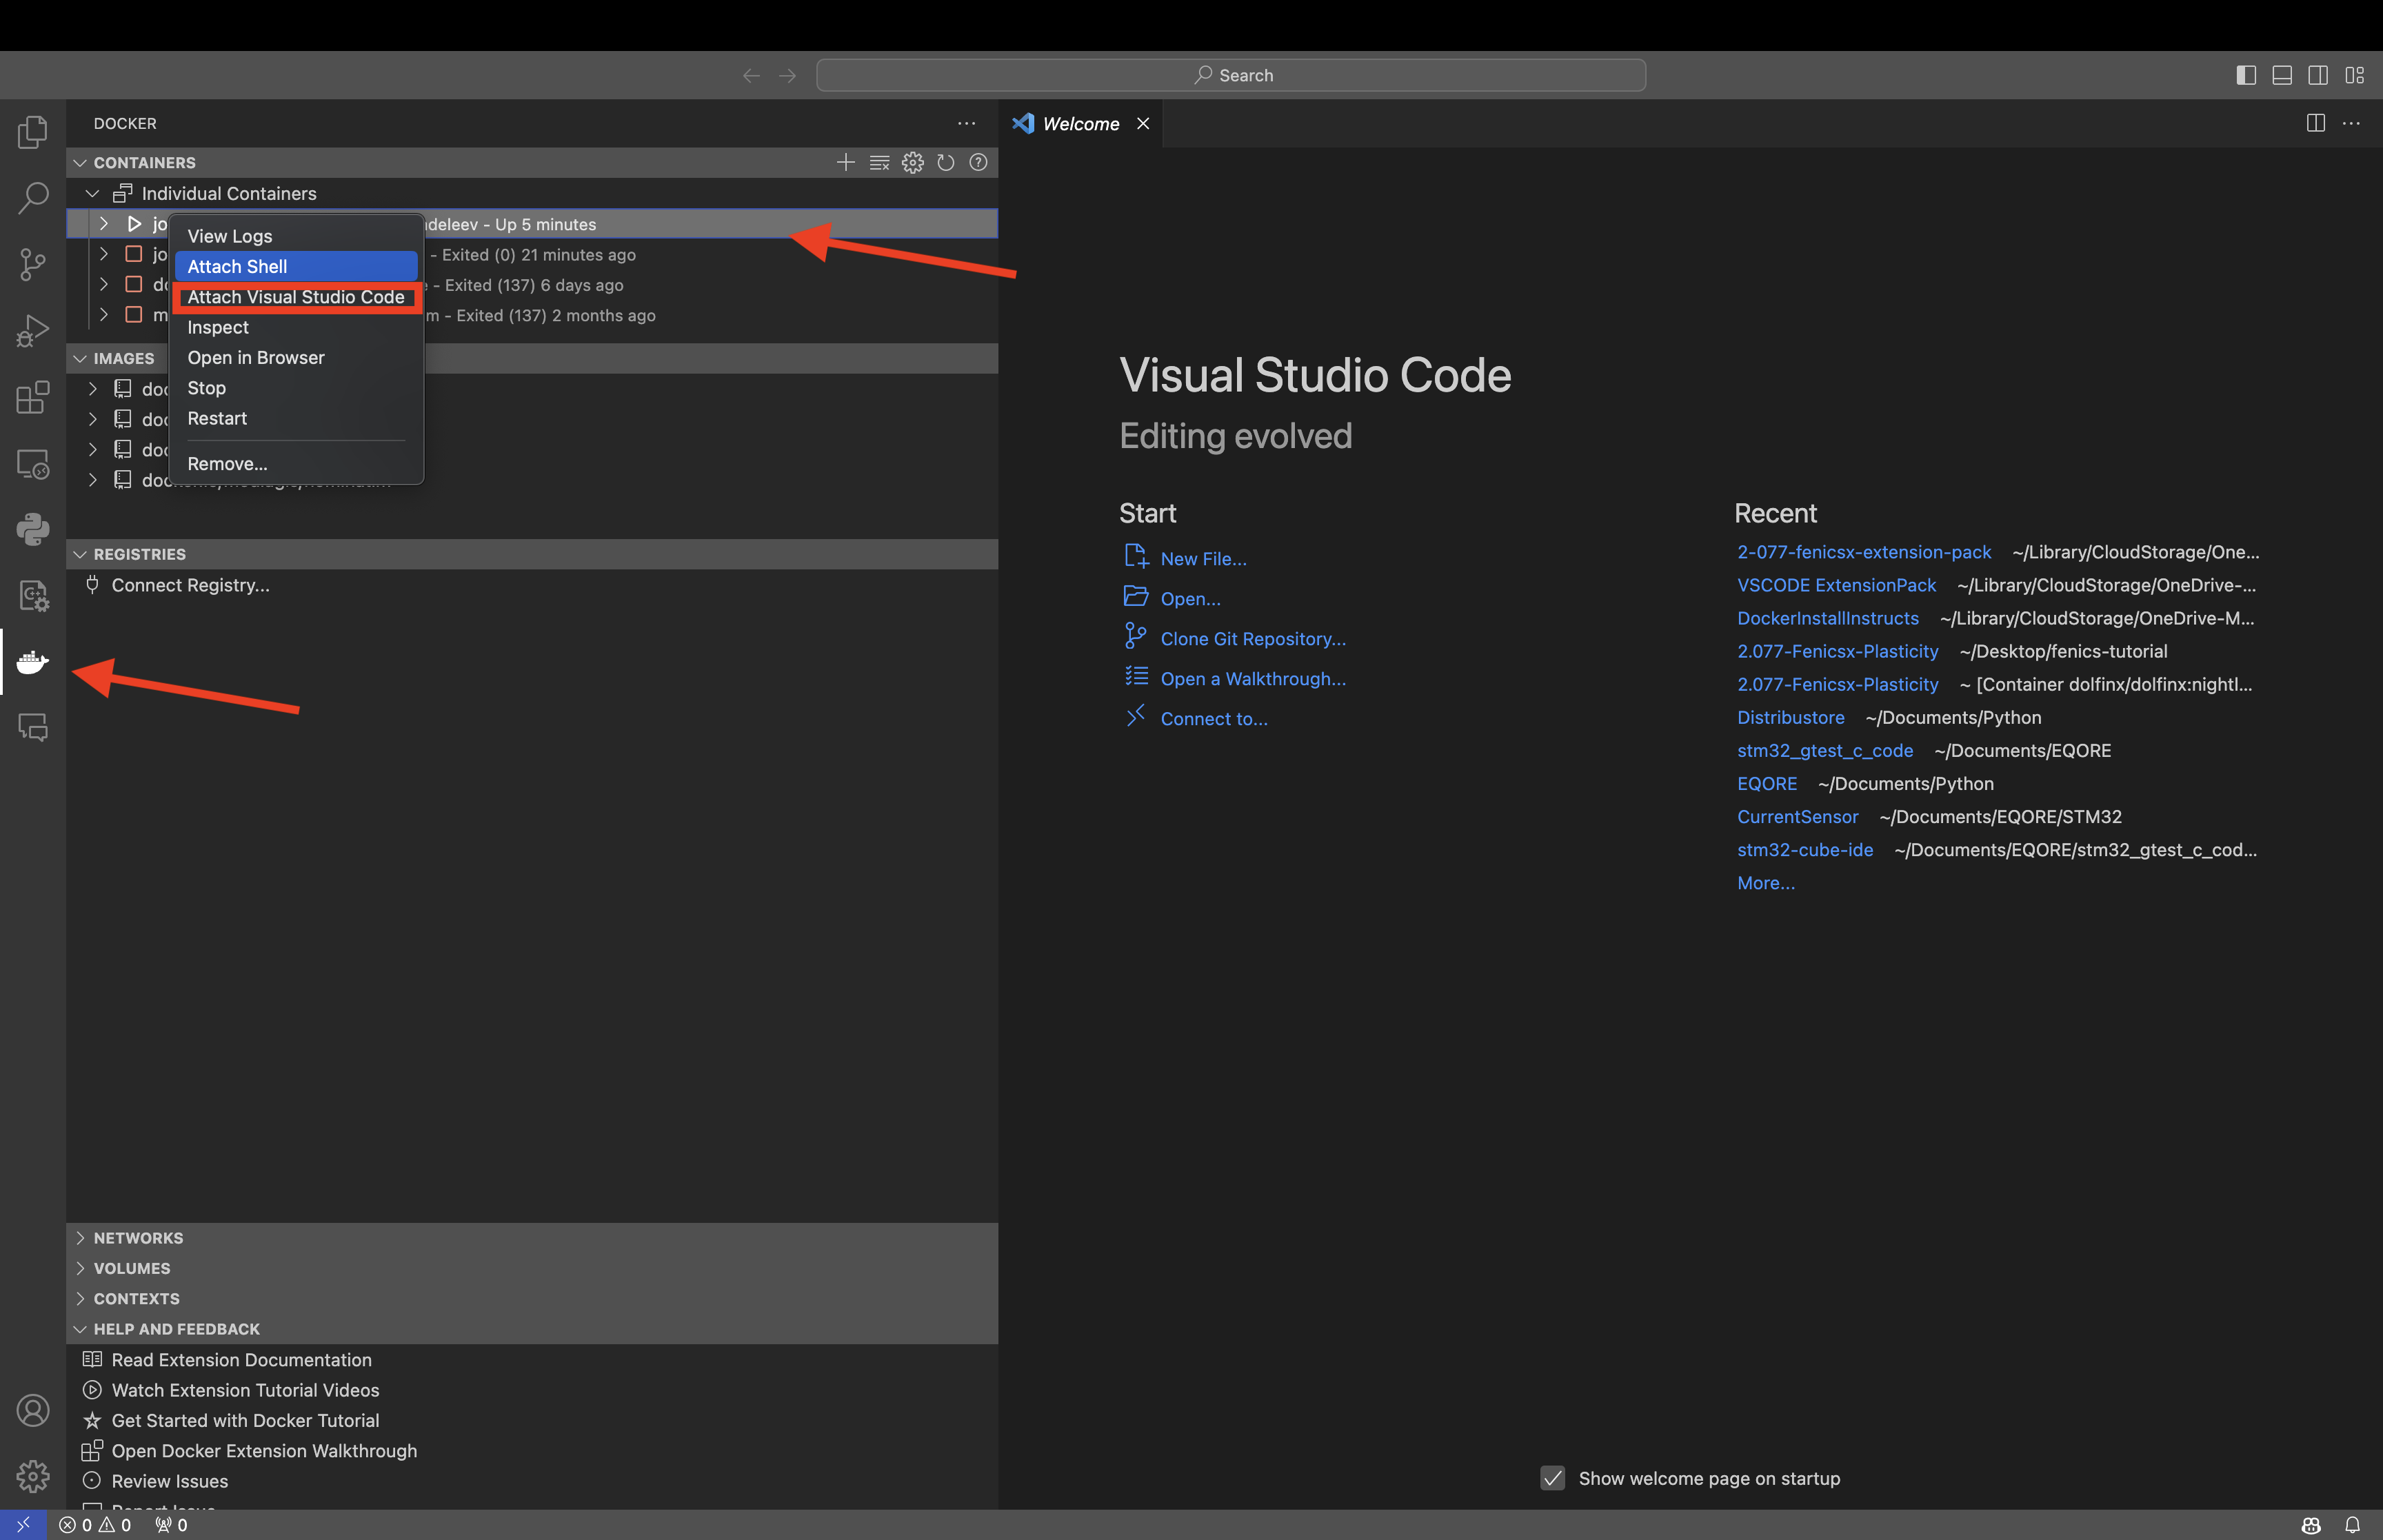
\includegraphics[width=0.7\textwidth]{VsCode-Docker.png}
  \caption{How to open up the docker extension and launch into the file. Right clicking on any of the containers will allow us to attach a VSCode instance. }%
  \label{fig:vsDocker}%
\end{figure}


This will open up a new tab of vscode. We can ensure we are connected by looking at the bottom left corner of the screen.
\begin{figure}[H]
  \centering
  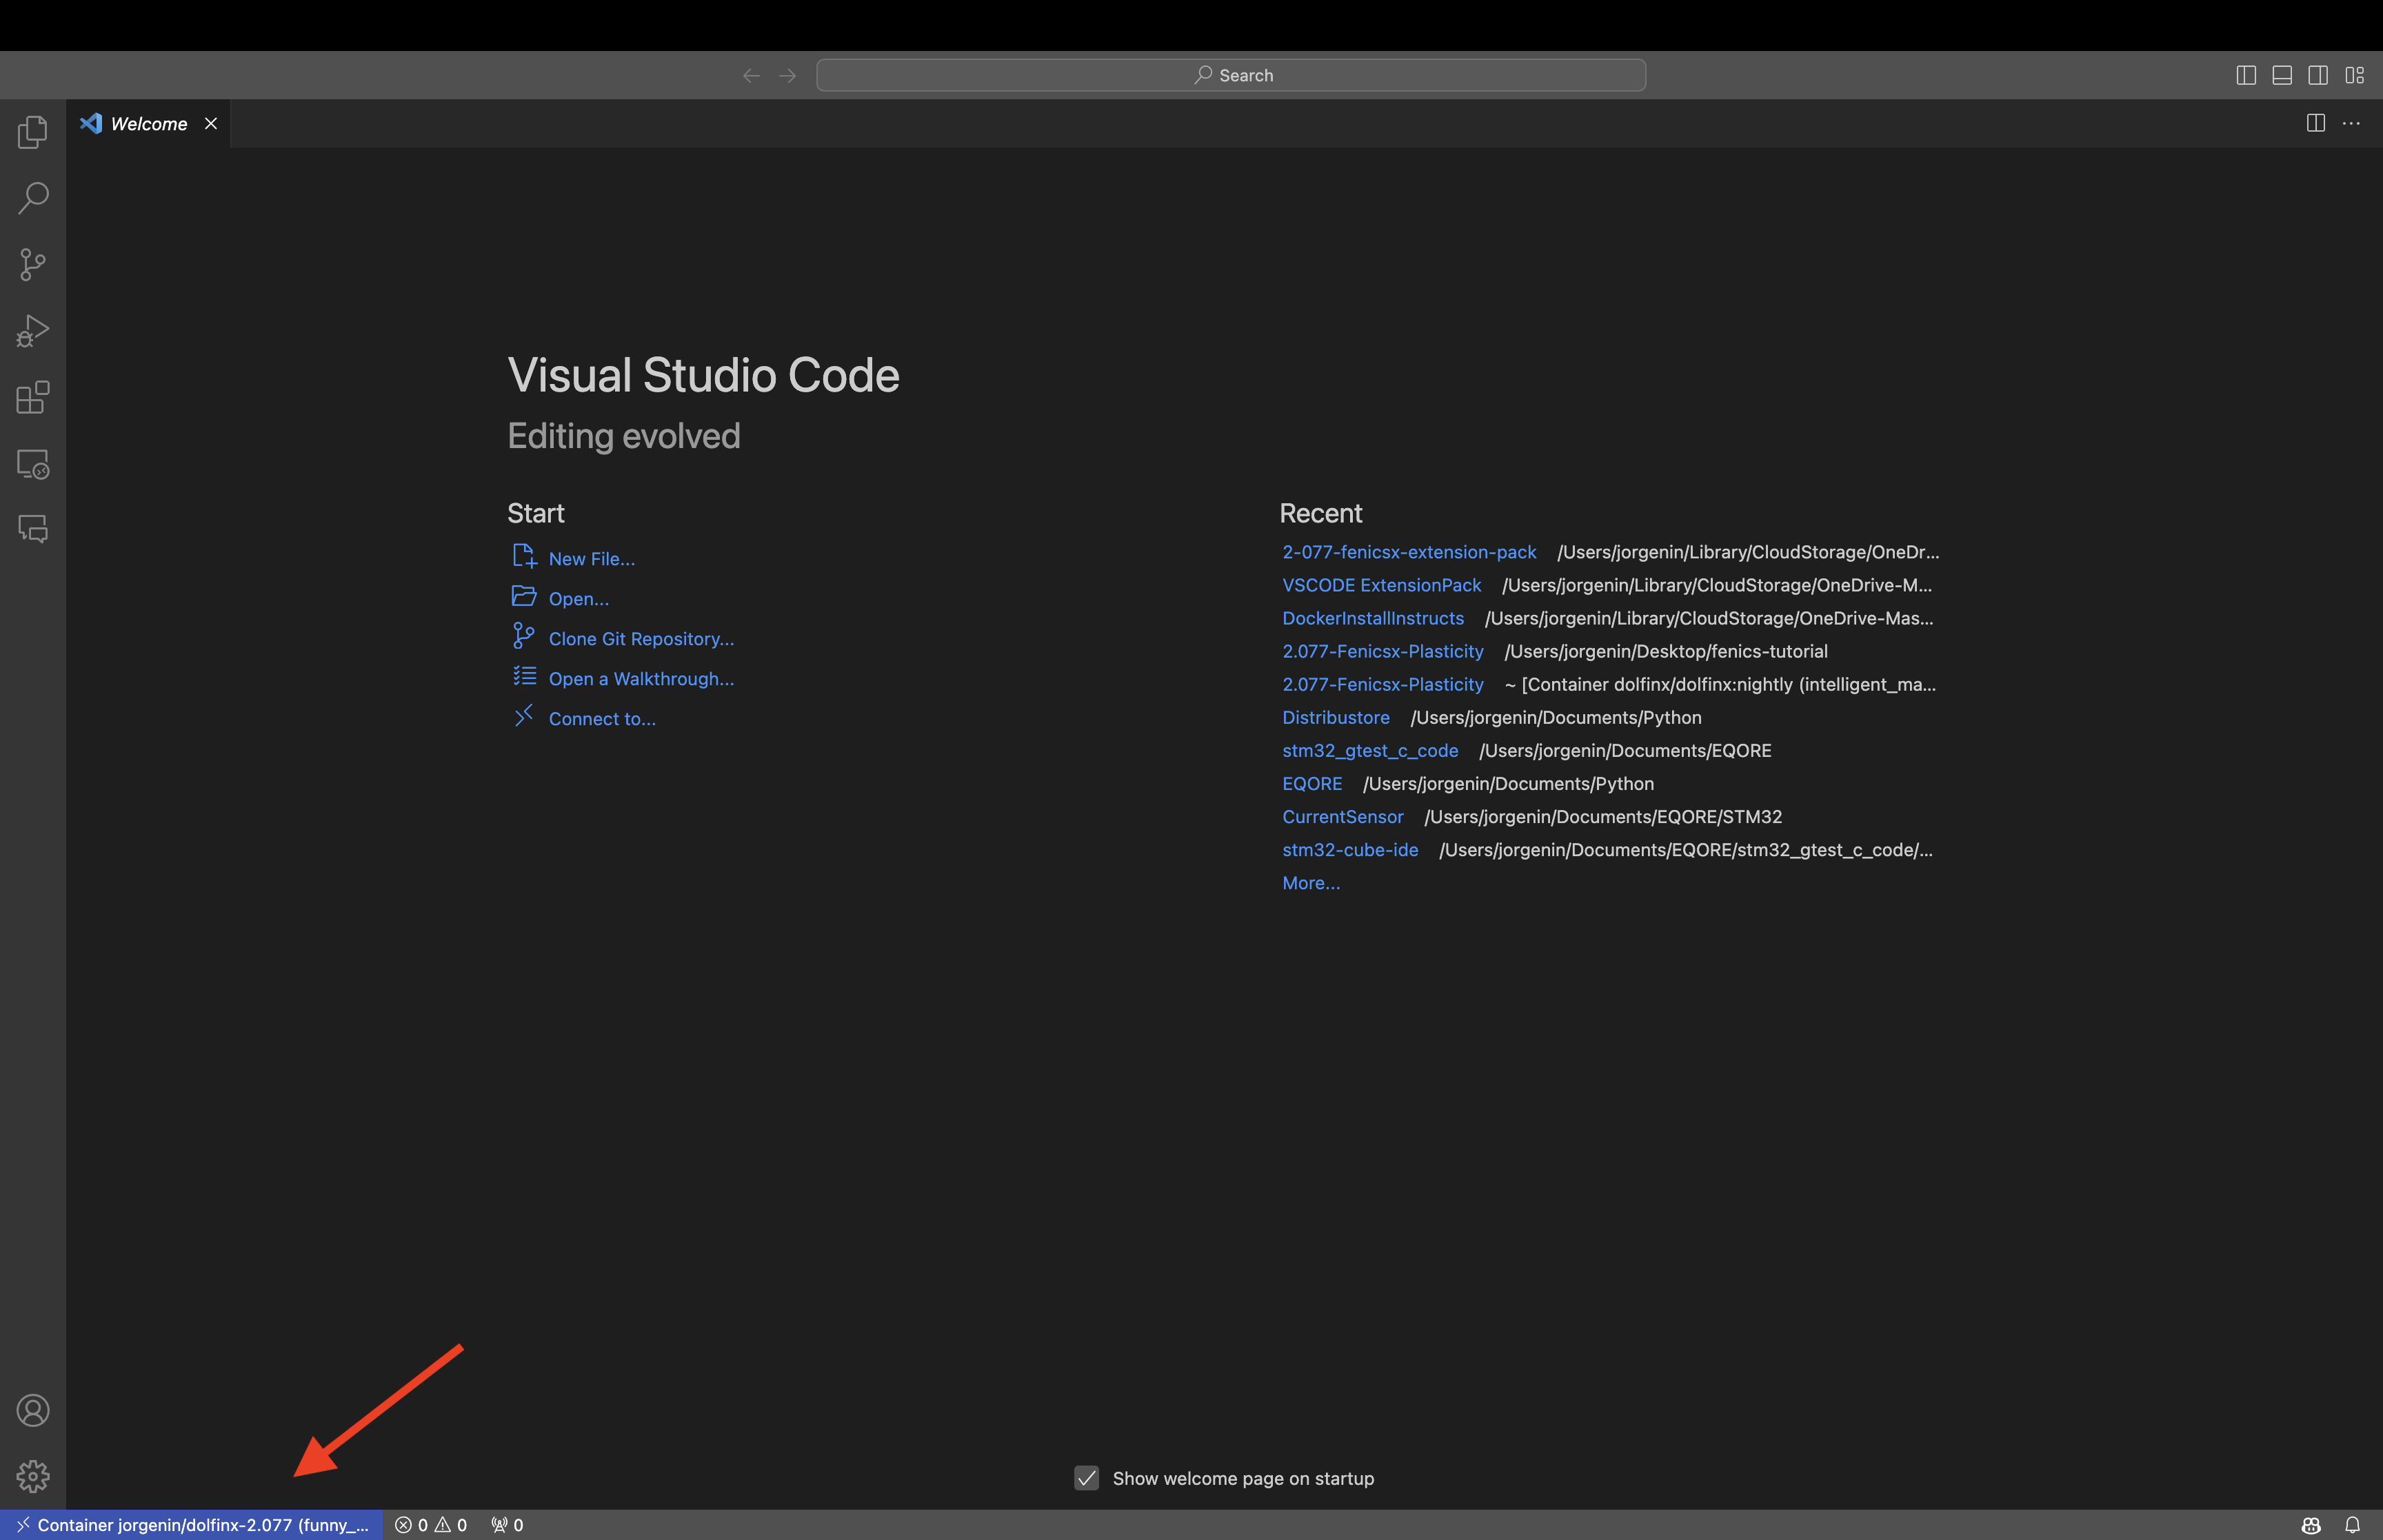
\includegraphics[width=0.7\textwidth]{VsCode-Connected.png}
  \caption{How to open up the docker extension and launch into the file. Right clicking on any of the containers will allow us to attach a VSCode instance. }%
  \label{fig:vsDocker-connected}%
\end{figure}

\subsection{Enabling Extensions In Container}
By default VSCode extensions are not installed in the container. To enable them we can just go to the exensions, and search for the 2.077 FeniCSx exension pack and insall it.

\begin{figure}[H]
  \centering
  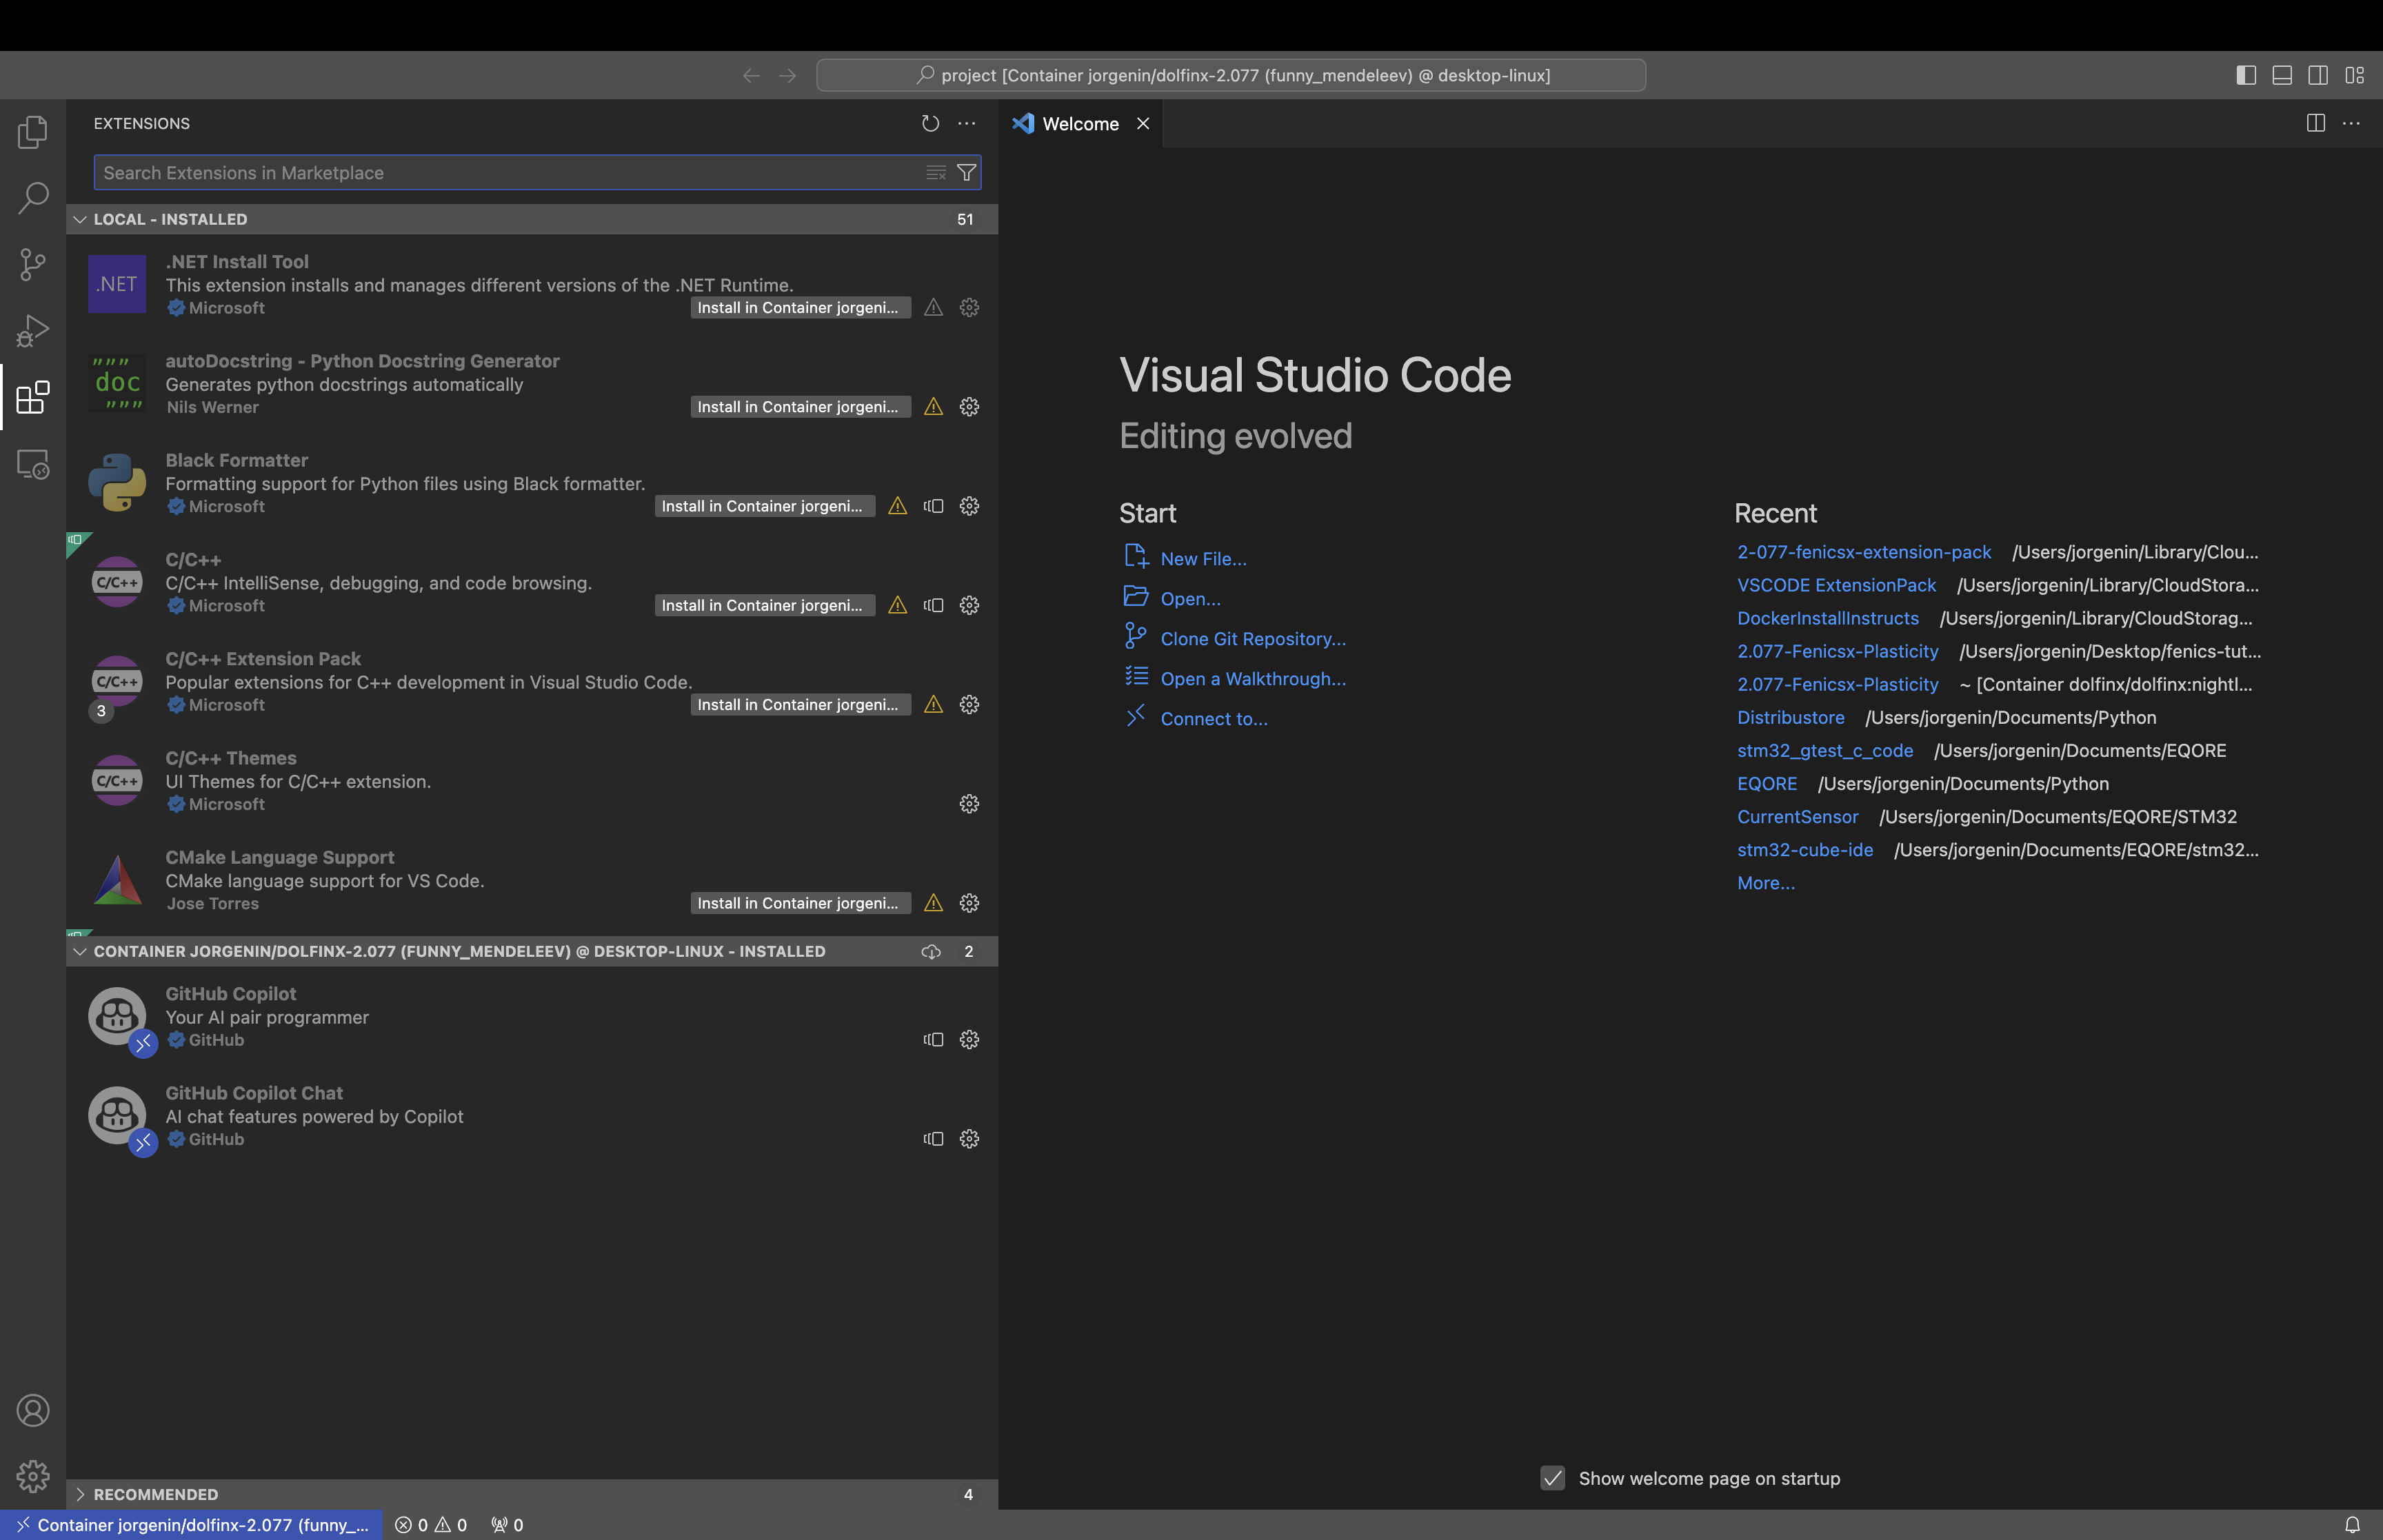
\includegraphics[width=0.7\textwidth]{Extensions-Container.png}
  \caption{Exensions in the host are not automatically carried over to the conatiner. It is the same process as before to install the extensions into the container. }%
  \label{fig:vsDocker-extension}%
\end{figure}

\subsection{Cloning a respository}

We can now open up our code with VSCode.

By default VS-Code connects to the root folder of the container. We normally want to avoid adding files into here if possible.
What we will do is use the terminal to clone a repository from git into the shared folder we created earlier.
We will then open that folder with vscode.

We can open up the terminal by click on the terminal tab on the top of the screen and then clicking on new terminal.

The terminal will open in the bottom of the screen.

\begin{figure}[H]
  \centering
  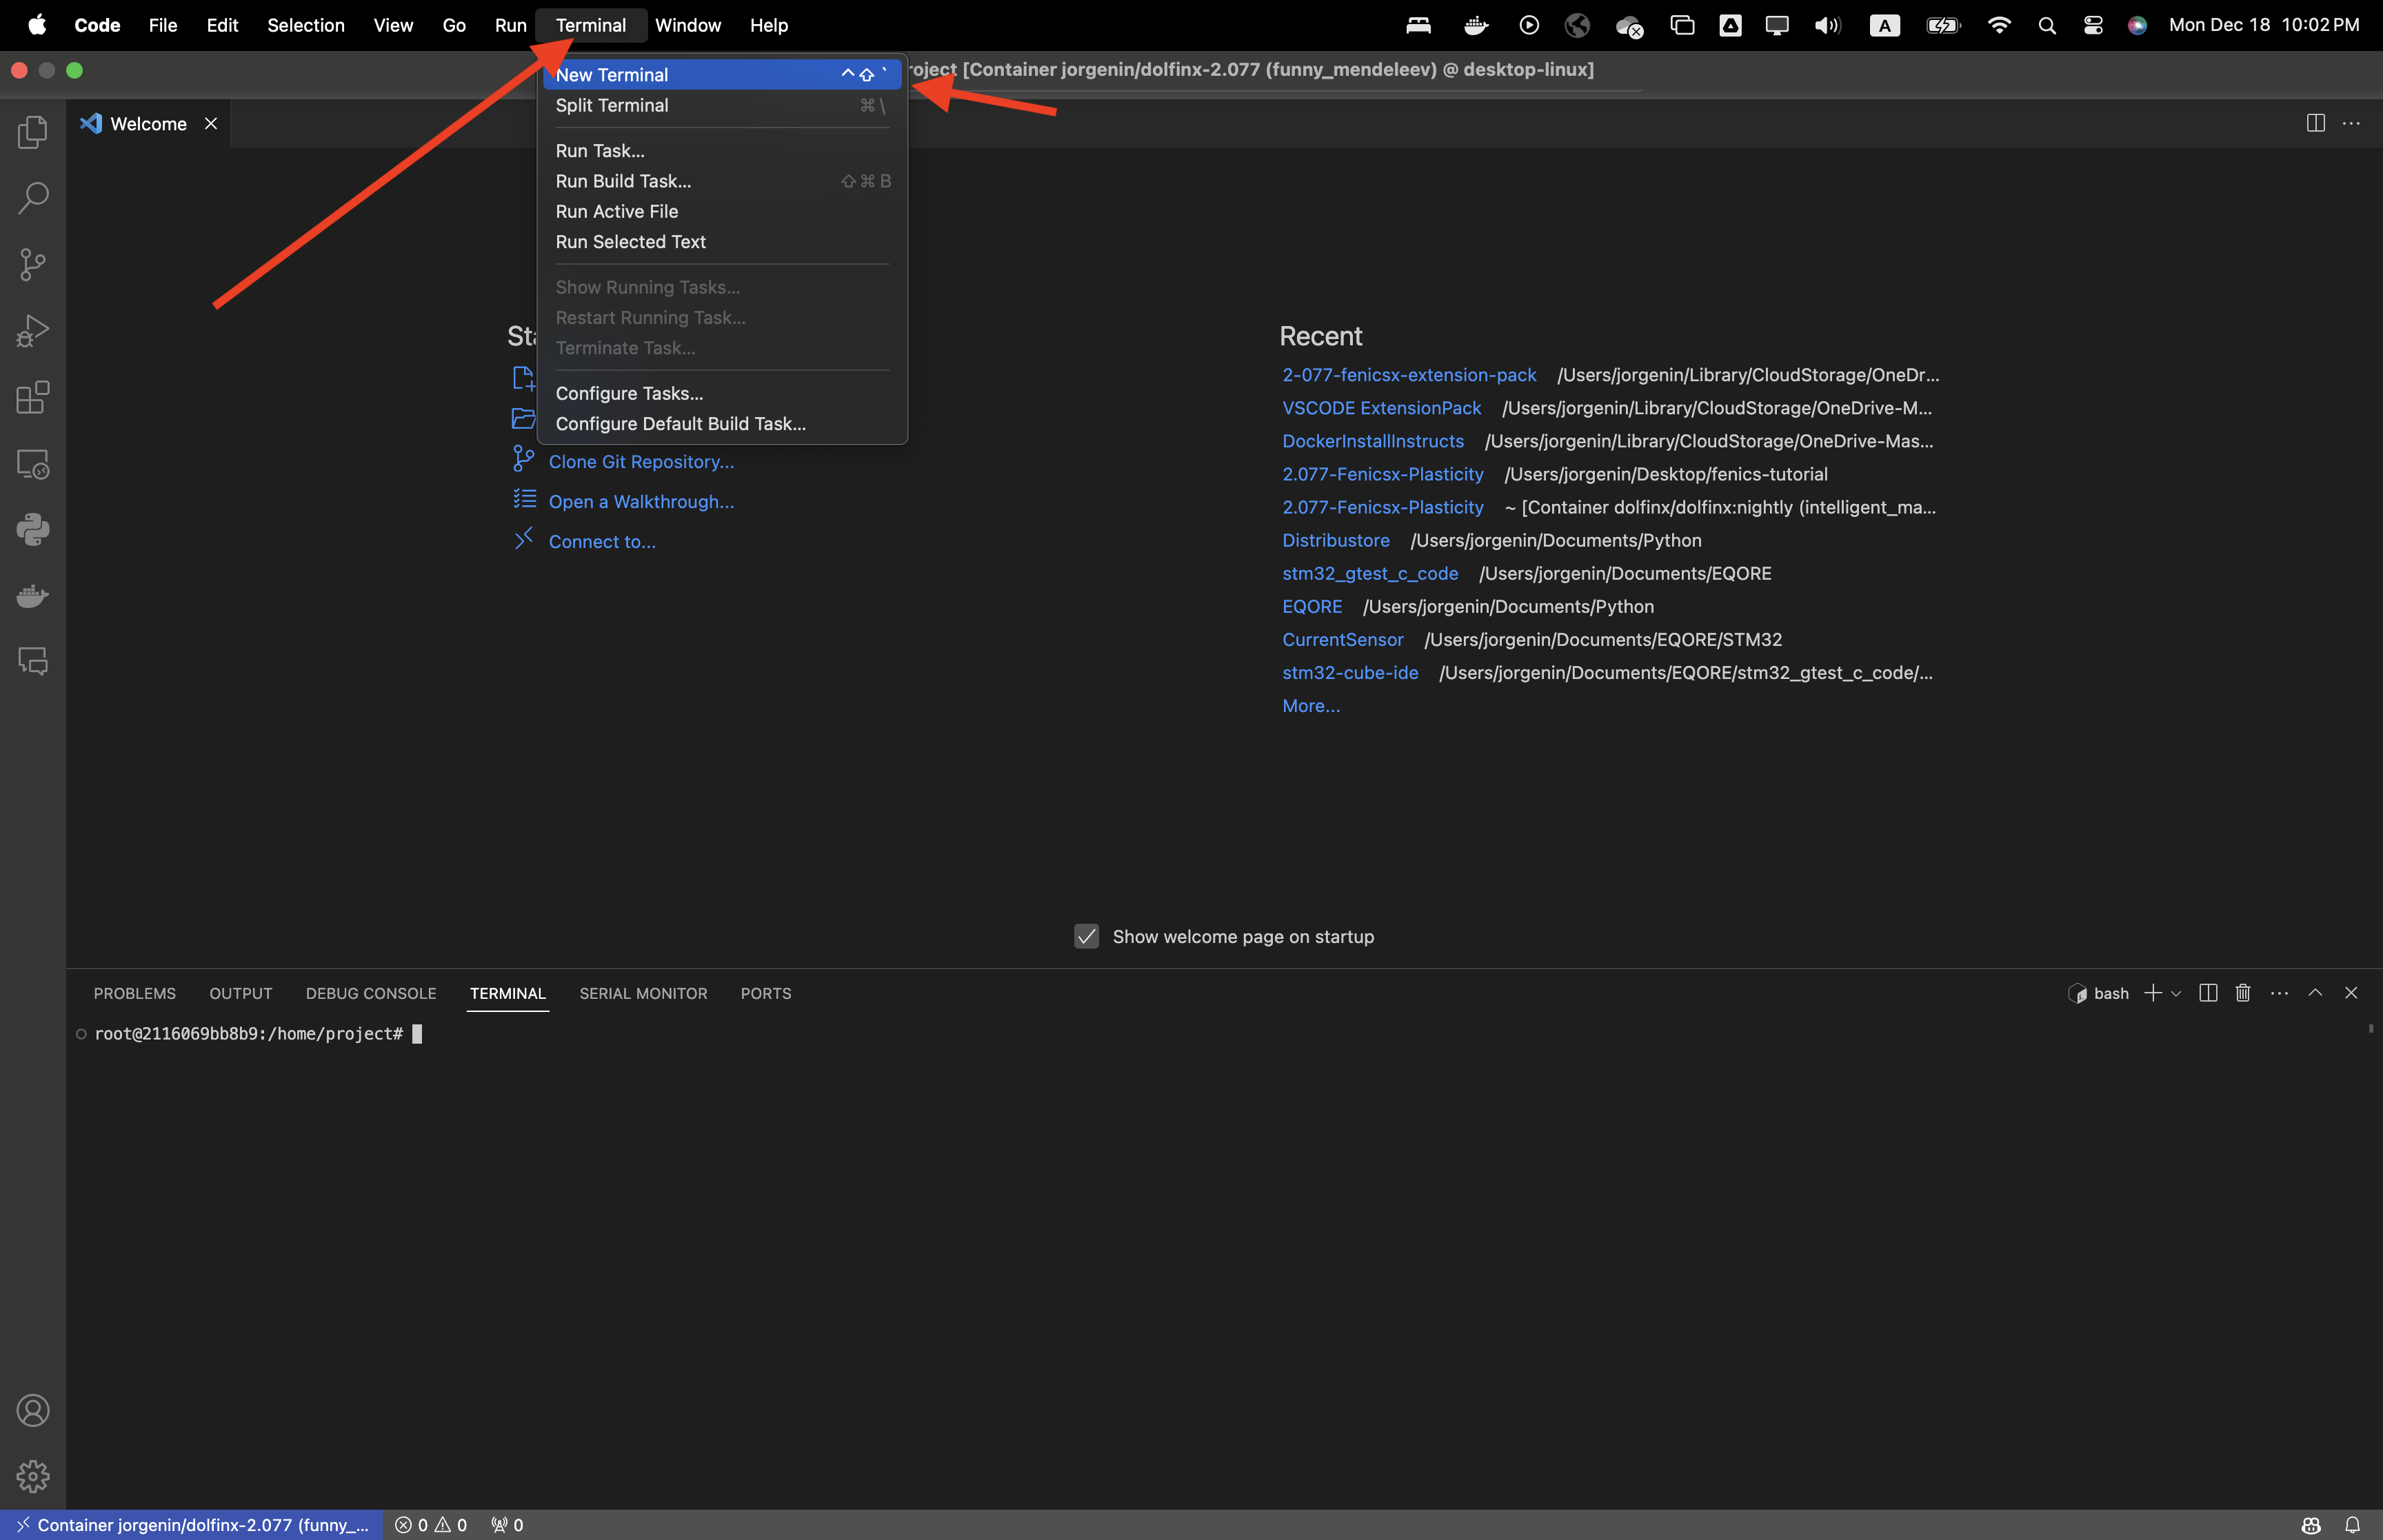
\includegraphics[width=0.7\textwidth]{Terminal-Open.png}
  \caption{How to open a Terminal in VSCode }%
  \label{fig:vsDocker-Terminal}%
\end{figure}


Our shared folder is \clist{/home/project} so we will navigate to it by running the following command:
\begin{lstlisting}[language=bash, caption=Docker Pull Command]
  > cd /home/project
\end{lstlisting}

We can then clone the repository by running the following command:
\begin{lstlisting}[language=bash, caption=Docker Pull Command]
  > git clone https://github.com/jorgenin/2.077-Fenicsx-Plasticity
\end{lstlisting}


\begin{figure}[H]
  \centering
  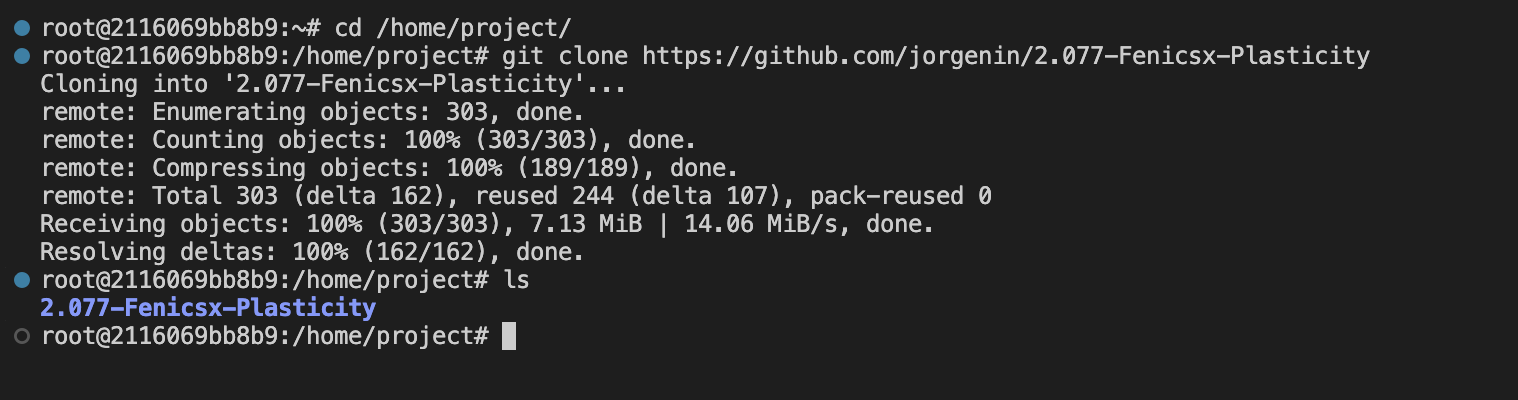
\includegraphics[width=0.7\textwidth]{terminal_output.png}
  \caption{Ouput from the terminal after running commands }%
  \label{fig:vsDocker-Terminal_ouput}%
\end{figure}


After Running the commands we can look in our host computer and see that the files were also in the shared folder.
This is because we created the files in our shared folder.

\begin{figure}[H]
  \centering
  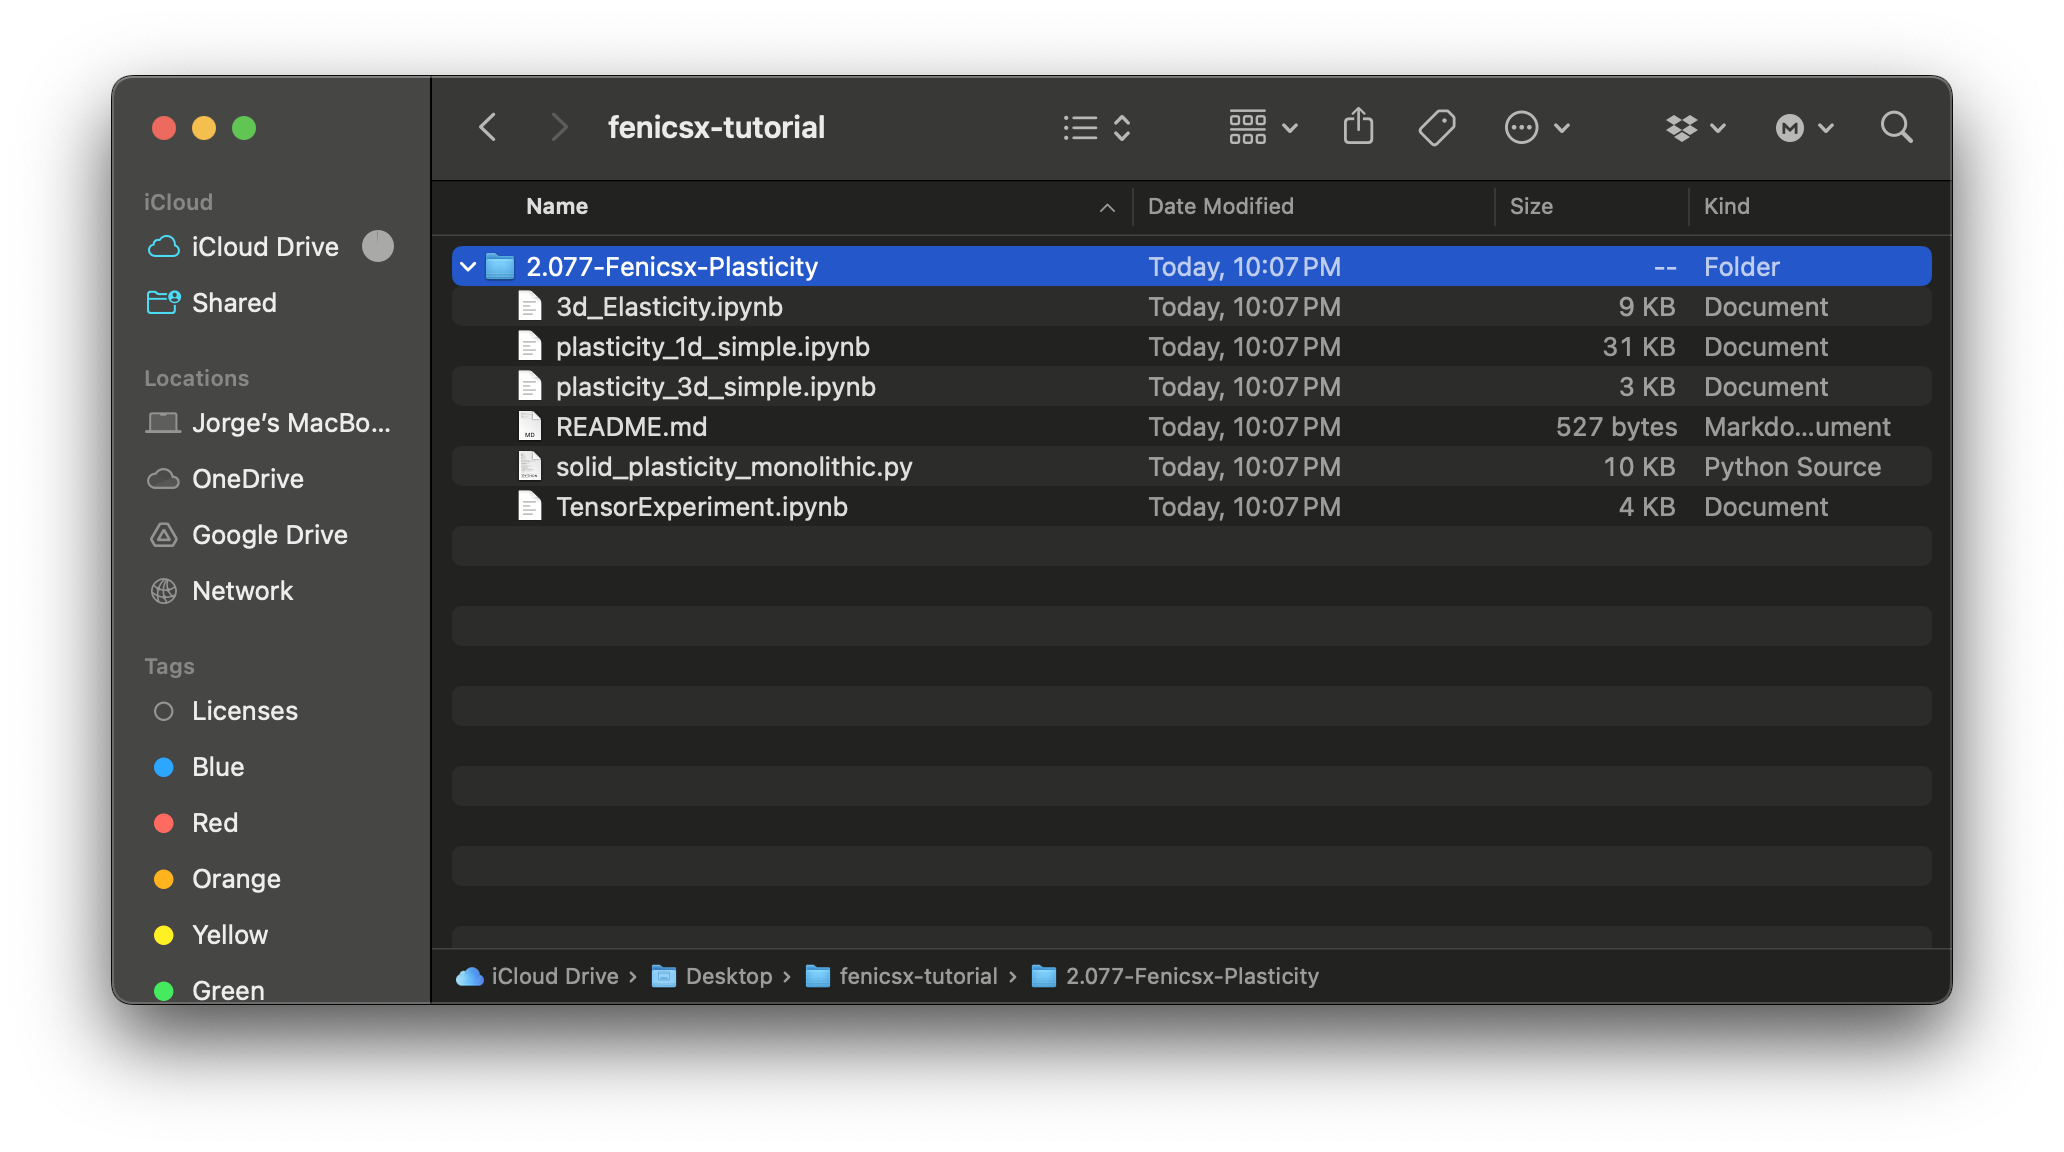
\includegraphics[width=0.7\textwidth]{Files-After-Git-clone.png}
  \caption{The git clone from the container also created the files in our shared folder. This is because we shared the folder initially when initializing the container.}%
  \label{fig:shared_files}%
\end{figure}

\subsection{Opening Folder and Running Example}

We can now open up the folder in vscode and run the example.

We can do this in two ways, either in the welcome screen we can click open, or we can click on file and then on open.
You can see this in figure \ref{fig:vsDocker-Open-Folder}.
\begin{figure}[H]
  \centering
  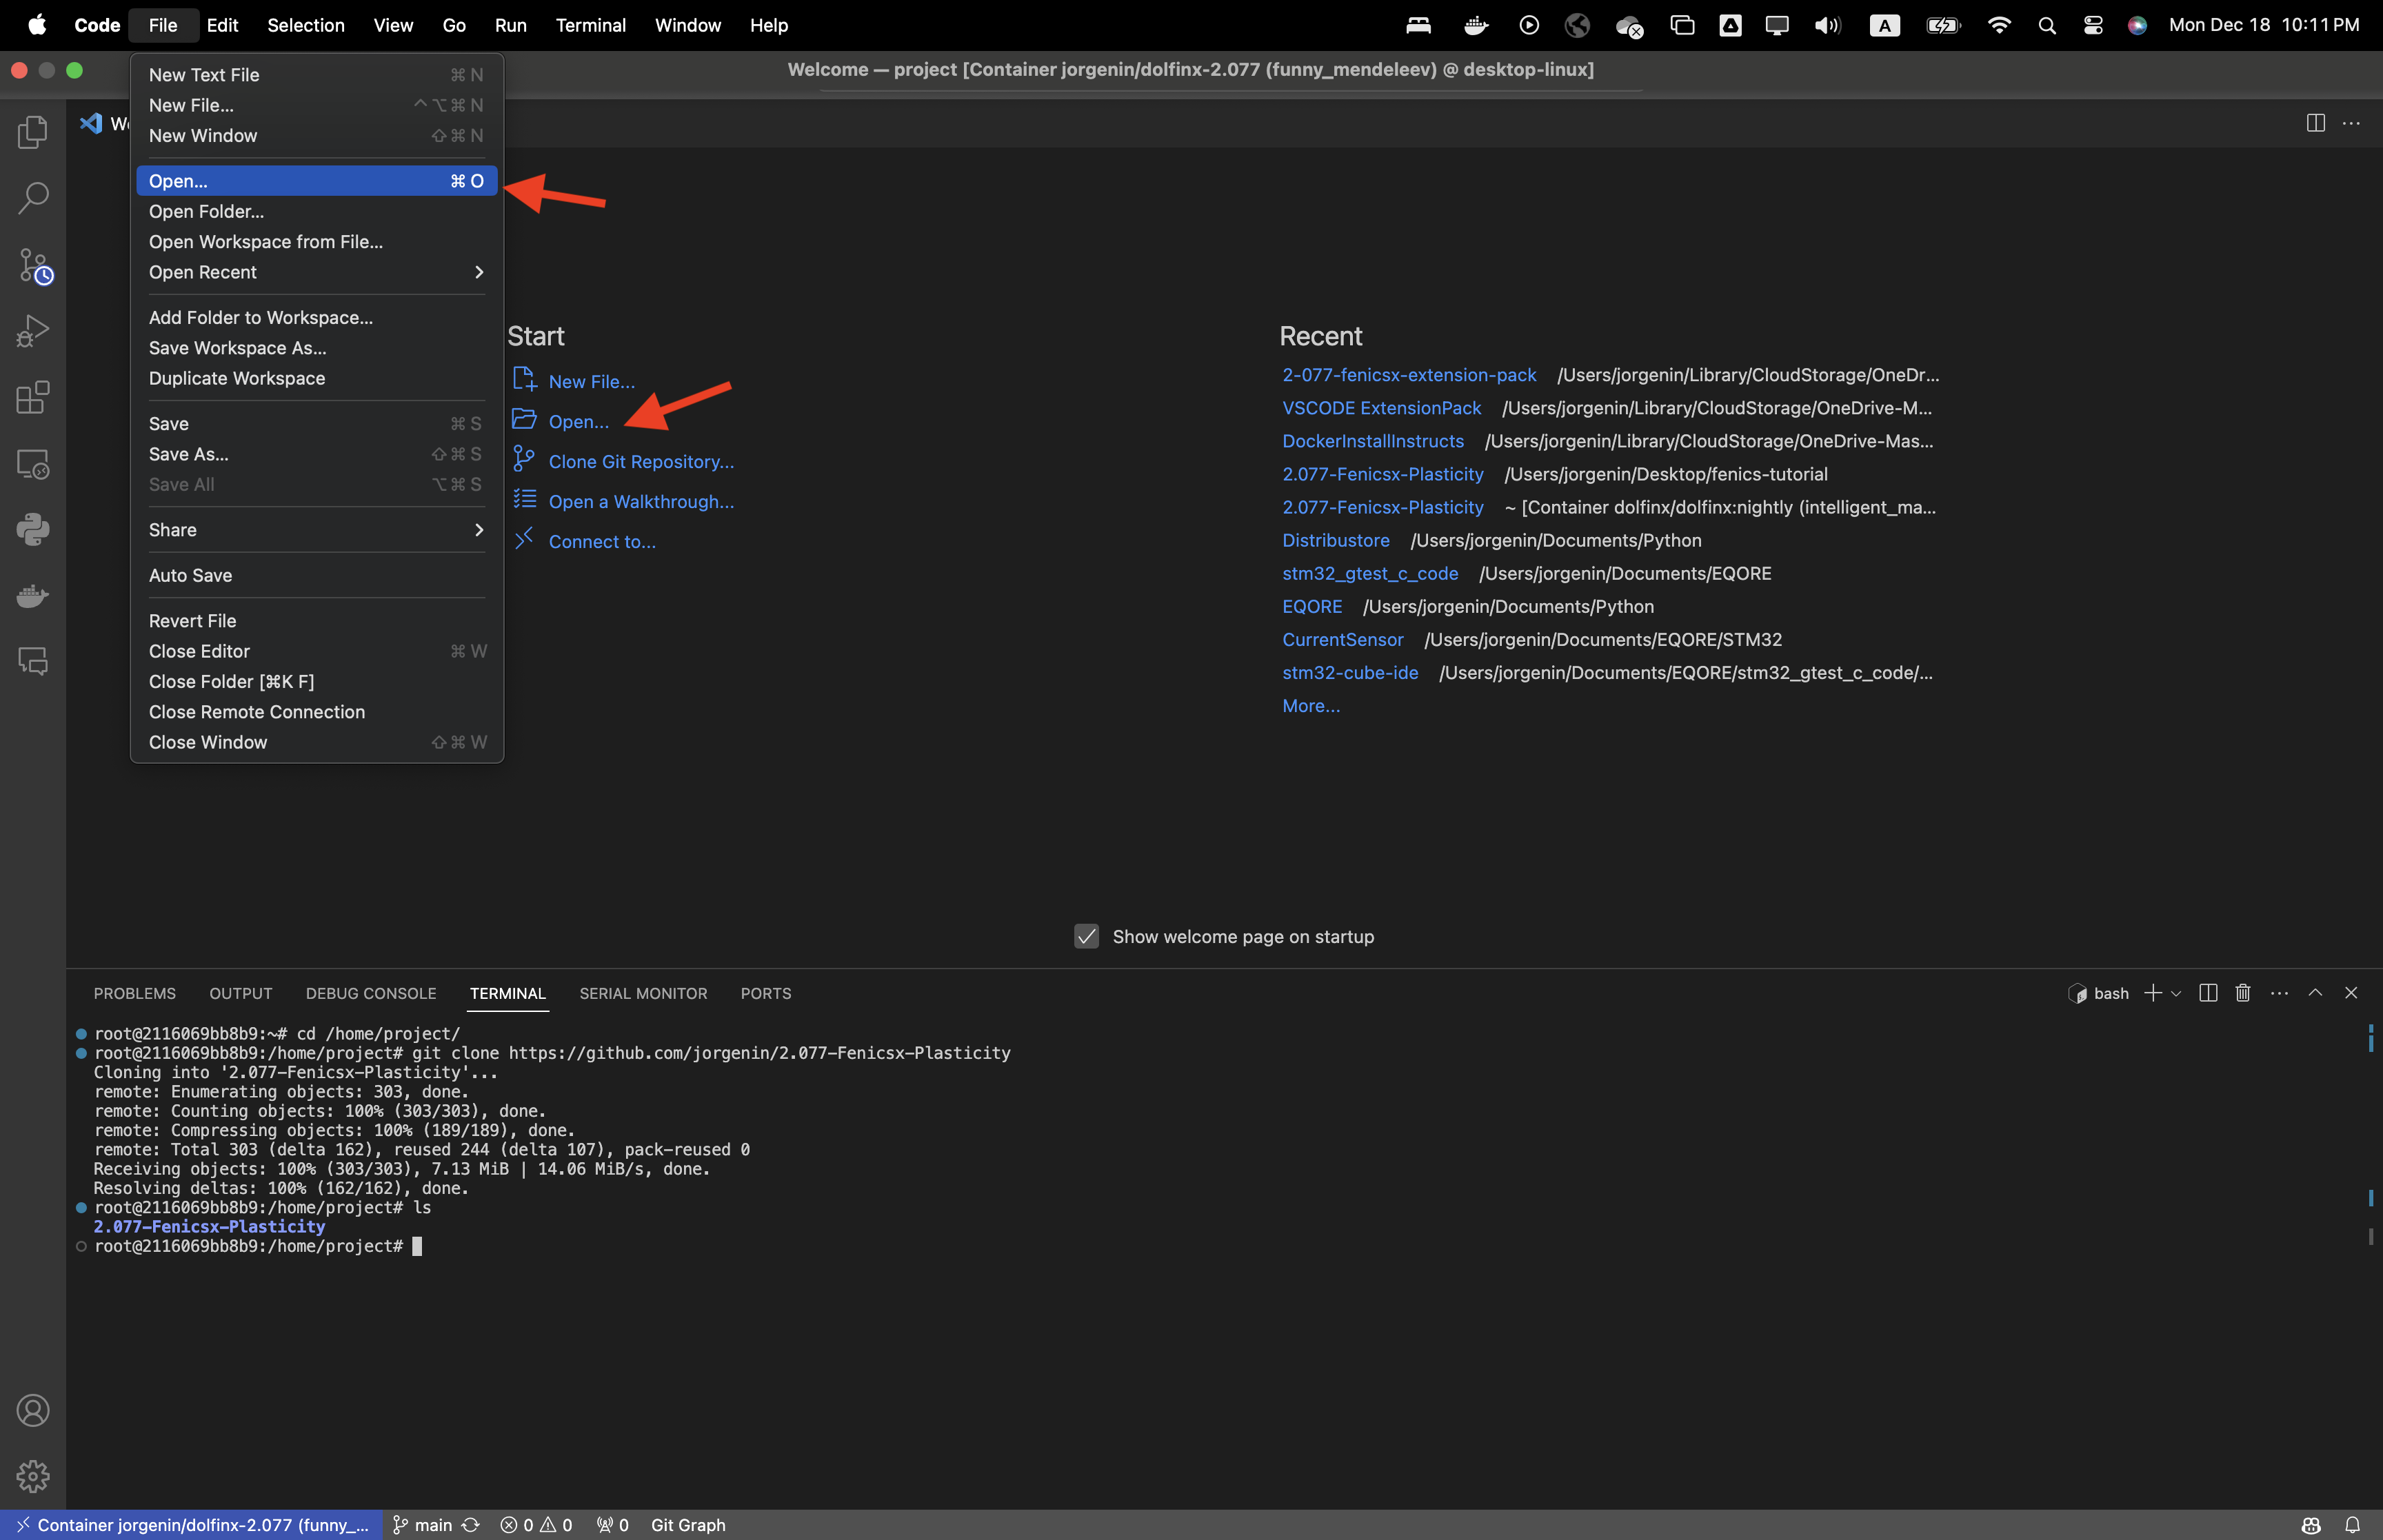
\includegraphics[width=0.7\textwidth]{Open-File.png}
  \caption{How to open a folder in VSCode }%
  \label{fig:vsDocker-Open-Folder}%
\end{figure}

Either method opens the same window where we can select the folder we want to open.
in this case we want to open the \clist{2.077-Fenicsx-Plasticity} folder.
\begin{figure}[H]
  \centering
  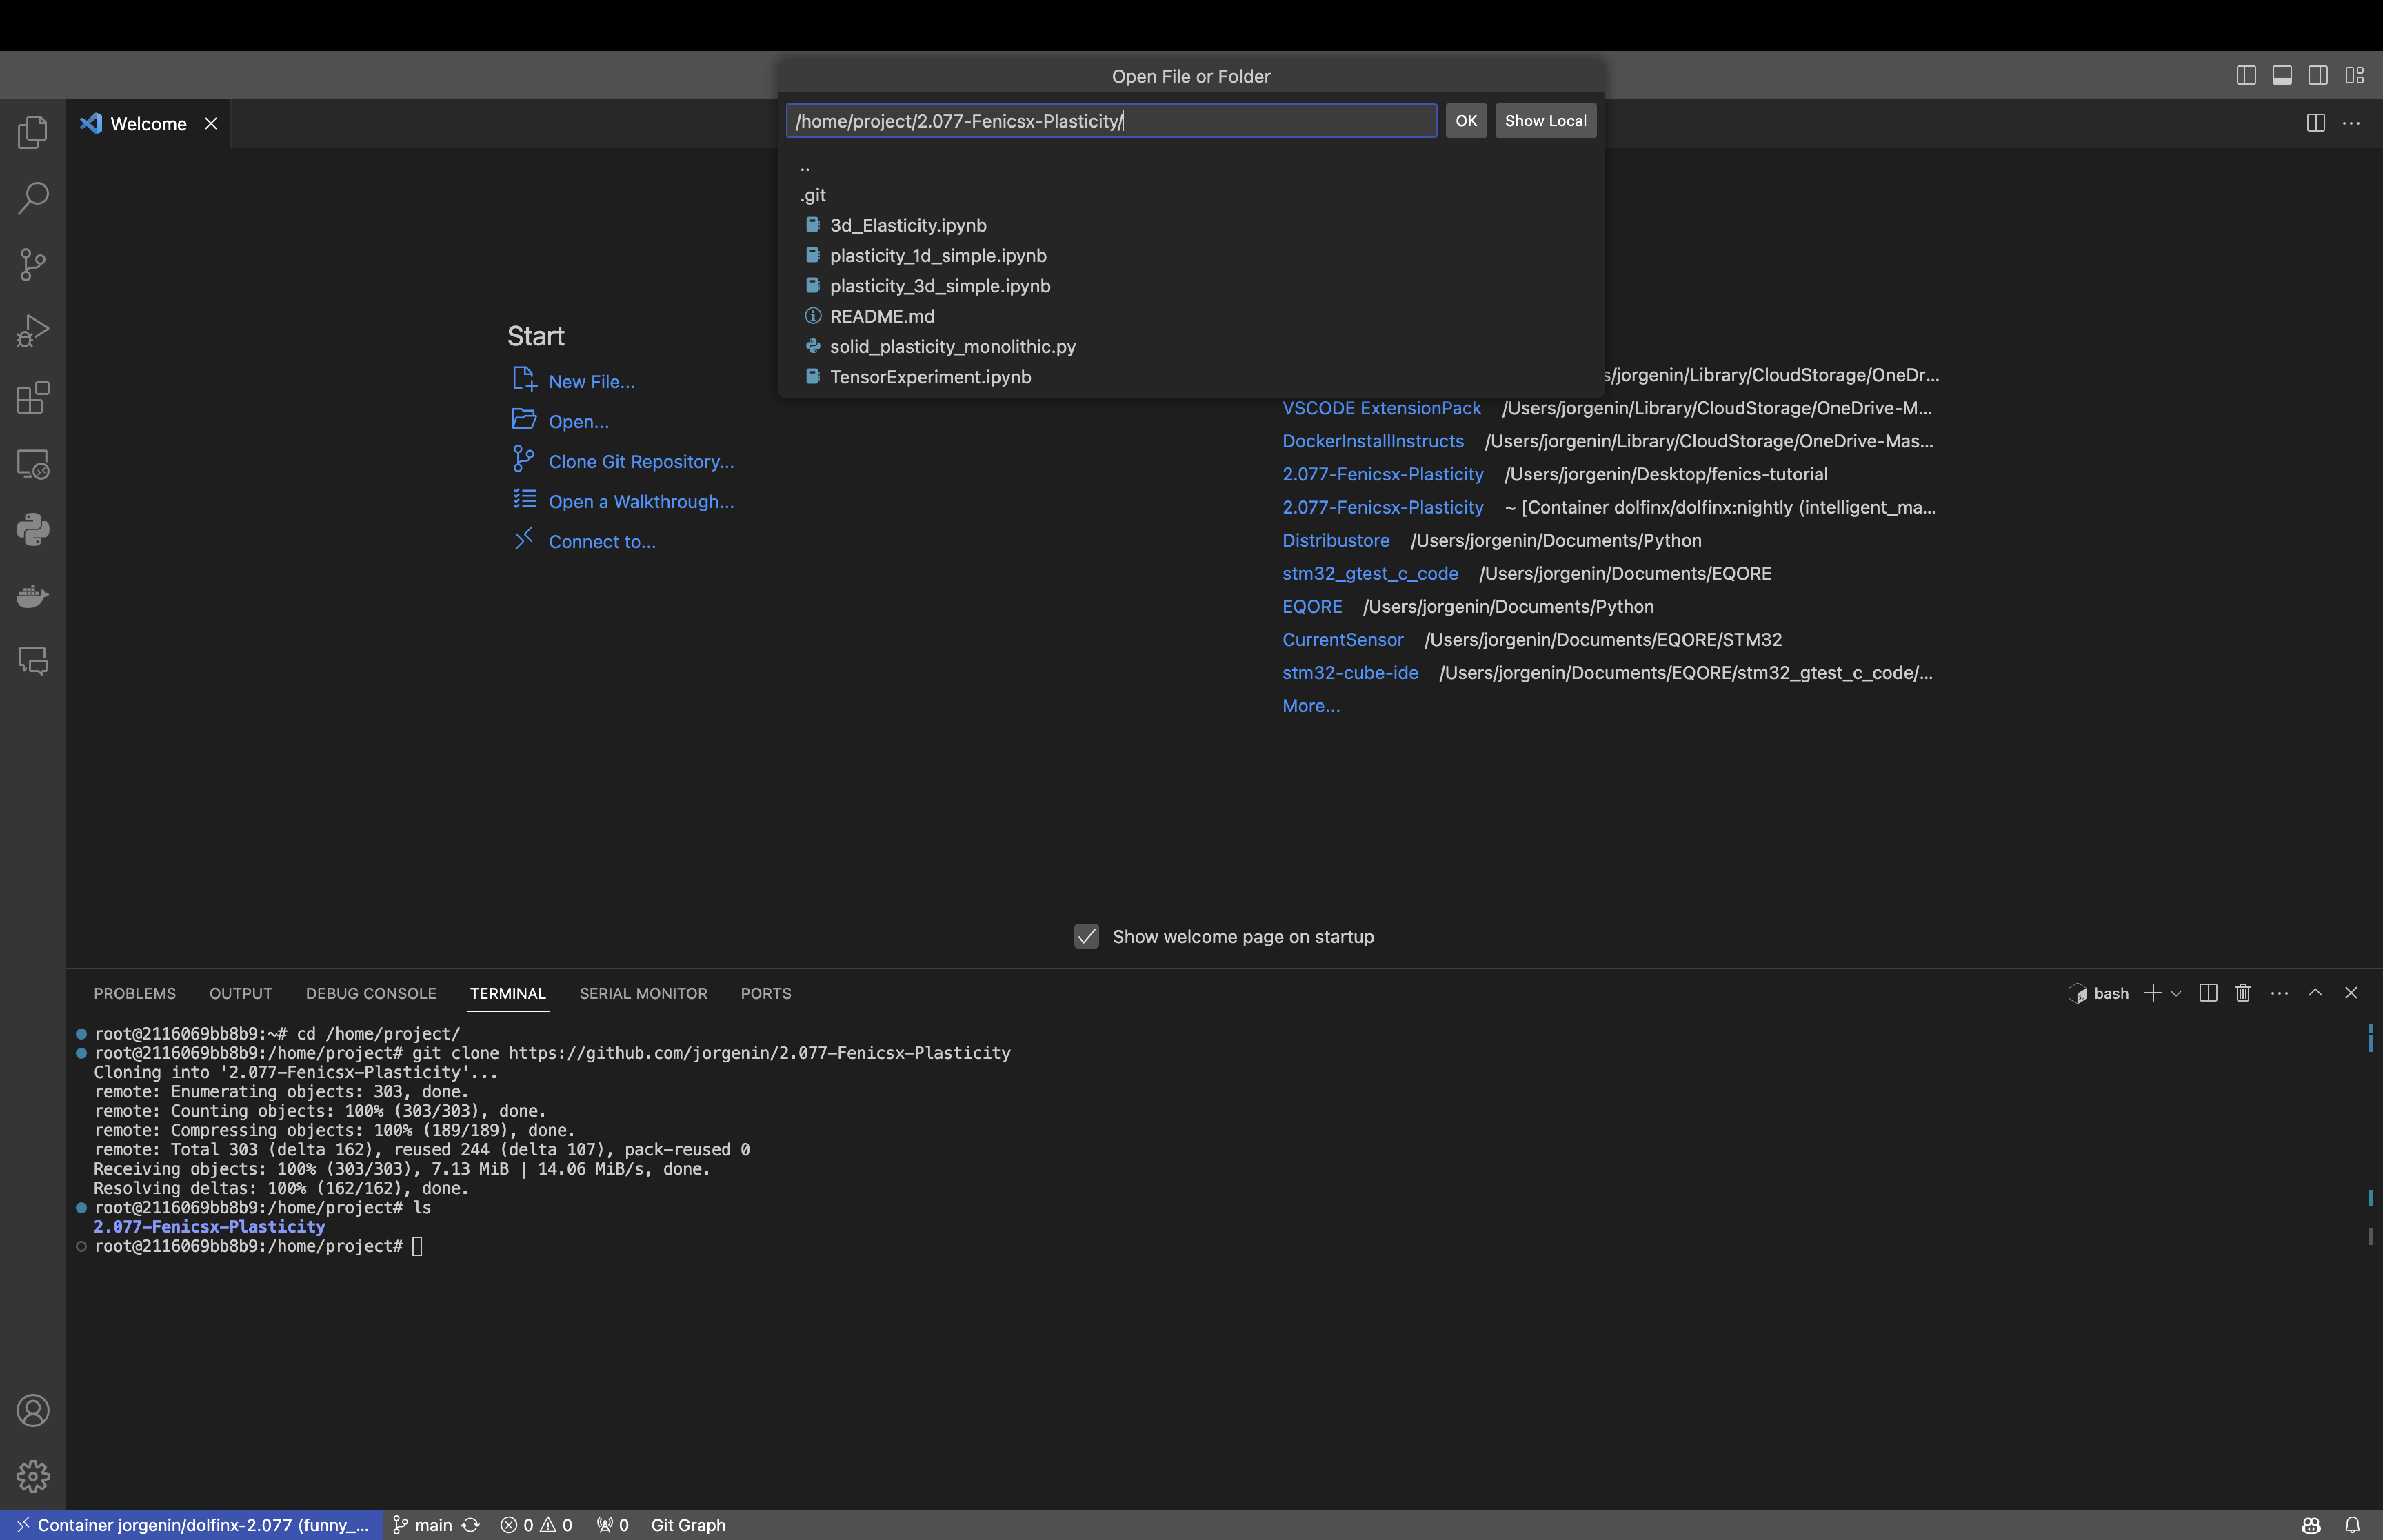
\includegraphics[width=0.7\textwidth]{Open-Folder-accept.png}
  \caption{Selecting the FeniCSx Plasticity folder }%
  \label{fig:vsDocker-Open-Folder-Accept}%
\end{figure}

We can now see the folder in the file explorer tab in VSCode. We can open up any file in the project and edit / or run it as necessary.

Jupyter notebooks will open inline. We can make sure we are using the right python verion (3.10 at the time of writing) and then clicking run all to run the entire example as seen in figure \ref{fig:Project_Open}.
\begin{figure}[H]
  \centering
  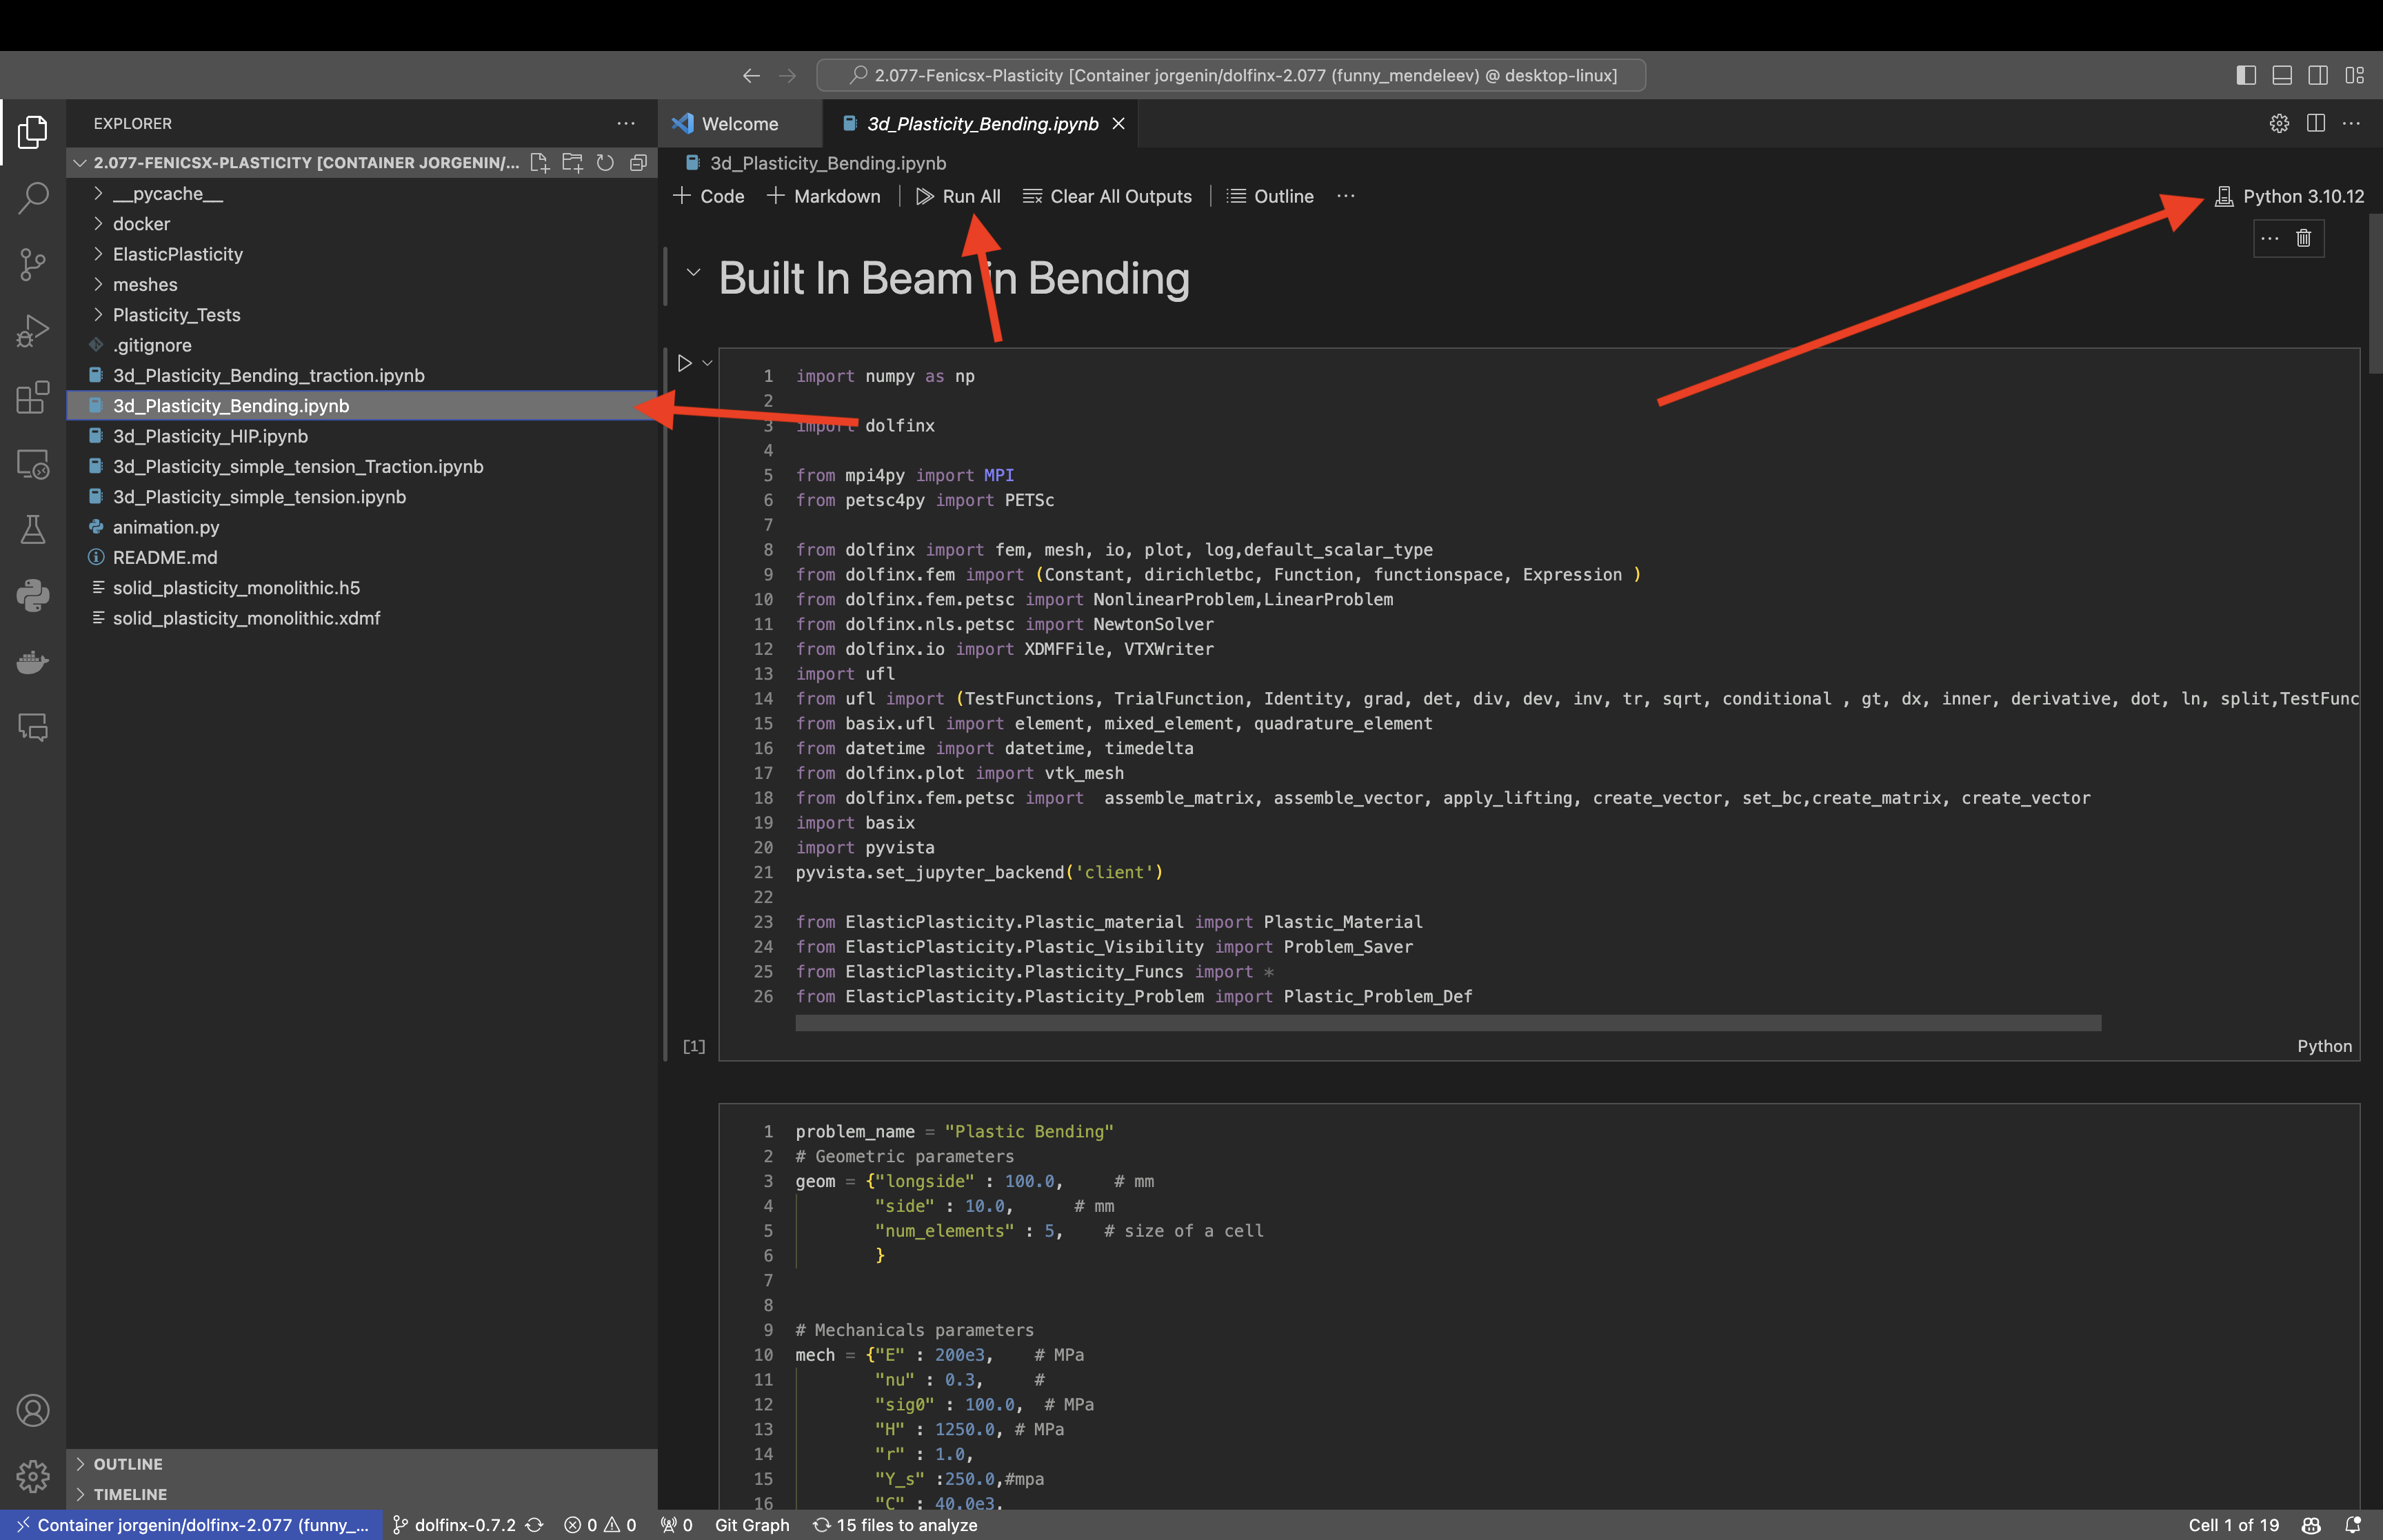
\includegraphics[width=0.7\textwidth]{VSCode-ProjectOpen.png}
  \caption{Running the Jupyter Notebook }%
  \label{fig:Project_Open}%
\end{figure}


\section{Appendix}
Here is a link to my github respository:
\href{https://github.com/jorgenin/2.077-Fenicsx-Plasticity}{GitHub FEniCSX Finite Plasticity}


\section{Creating a new Docker Image}

From time to time you may want to create you're own custom docker image. For example if there is a new update to FEniCSx or if you want specific dependencies automatically intstalled in an image.
This section will be covering how to do this, and then uploading that image to DockerHUB, to share the image with others.

\subsection{Docker Files}
Images are normally defined by docker files. These are essentially a list of commands that docker will run to create the image.
You can find the docker file that was used in this tutorial \href{https://github.com/jorgenin/2.077-Fenicsx-Plasticity/blob/main/docker/dockerfile}{here}.

\begin{lstlisting}[language=bash]
FROM dolfinx/dolfinx:nightly
ARG TARGETARCH
SHELL ["/bin/bash", "-c"]
LABEL maintainer="Jorge Nin <jorgenin@Mit.edu>"

# Install dependencies
RUN apt-get update && apt-get clean && apt-get install -y \
    xvfb vim ffmpeg


# Install python dependencies
RUN pip3 install --upgrade pip

RUN if [[ ${TARGETARCH} =~ "arm64" ]]; then \ 
    pip3 install "https://github.com/finsberg/vtk-aarch64/releases/download/vtk-9.2.6-cp310/vtk-9.2.6.dev0-cp310-cp310-linux_aarch64.whl";\
    fi


RUN pip3 install "pyvista[all,trame]" jupyterlab ipython ipywidgets

WORKDIR /home/project
\end{lstlisting}
\clist{FROM} declares what the base image we will be using is.
\clist{FROM dolfinx/dolfinx:nightly} will create the image from the nightly version of FEniCSx. We could also use \clist{FROM dolfinx/dolfinx:latest} to get the latest stable version of FEniCSx.
\clist{ARG TARGETARCH} is a command that stores the target architecture (eithr amd64 or arm64) into a variable we can access.

\clist{RUN} just runs a command in the "terminal" of the image.
\clist{WORKDIR} sets the default working directory of the image.

\subsection{Building the Image}
Once you've modified the docker file to your liking you can build the image by running the following command:
\begin{lstlisting}[language=bash]
  > docker build -t "image name" .
\end{lstlisting}
Here \clist{"image name"} will be the name of the image you create.

You can than use this image as normal to create a container and use it for development.

\subsubsection{Building an image for different architectures}
By default the image you build is only for the architecture you are currently running on.

However we may want to build one image for arm64 and another for amd64 for exmaple so that both intel and M1 macs and use the image.
Doing this is a bit more invovled but not too difficult.

First we must create a custom builder that can cross compile the images.
We can do this by running the following command:
\begin{lstlisting}[language=bash]
  > docker buildx create --name mybuilder --bootstrap --use
\end{lstlisting}

We can then run the \clist{docker build ls} command to see the builders.
It should output something like this:
\begin{lstlisting}
  docker buildx ls
NAME/NODE     DRIVER/ENDPOINT              STATUS   BUILDKIT PLATFORMS
mybuilder *   docker-container
  mybuilder0  unix:///var/run/docker.sock  running  v0.12.1  linux/amd64, linux/amd64/v2, linux/amd64/v3, linux/arm64, linux/riscv64, linux/ppc64le, linux/s390x, linux/386, linux/mips64le, linux/mips64, linux/arm/v7, linux/arm/v6
default       docker
  default     default                      running  v0.12.3  linux/amd64, linux/arm64, linux/arm/v7, linux/arm/v6
\end{lstlisting}

We can then build the multiple images like so:

\begin {lstlisting}
docker buildx build --platform linux/amd64,linux/arm64 -t <username>/<image>:latest --push .
\end{lstlisting}

This will build the image for both amd64 and arm64 and then push it to docker hub.
We will talk more about pushing to docker hub in the next section.

\subsection{Pushing to Docker Hub}
Once we've created the image, and tested we may want to share it with others.

We can do this by pushing it to docker hub.
\href{https://hub.docker.com/repository/docker/jorgenin/dolfinx-2.077/general}{Here is the docker hub for the image we've used in this example.}
Opening the page you can see the different tags that we have availble.

As a part of pushing to dockerhub you must create an account.

After you've created an account and logged in through the docker dashboard, you may use the docker push command.
To do so first we must tag the images.
Normally images are named according to the following format:

\clist{<username>/<imagename>:<tag>}
The tag can be the verison of the image, or any other tag that describes the difference.

We can tag our image in two ways, during building or aftewards.

\subsubsection{Tagging during building}
During building we can tag our image with the \clist{-t} flag. We can actually tag the same image with multiple flags.

For example we can run the following command:
\begin{lstlisting}
  docker build  -t jorgenin/dolfinx-2.077:v0.8 -t jorgenin/dolfinx-2.077:latest -t jorgenin/dolfinx-2.077:v0.8.1 -t jorgenin/dolfinx-2.077:nightly .
\end{lstlisting}

And we will actually tag the image with \clist{v0.8}, \clist{latest}, \clist{v0.8.1}, and \clist{nightly}.

\subsubsection{Tagging after building}
We can tag the image after building by running:
\begin{lstlisting}
  docker tag <image id> <username>/<imagename>:<tag>
\end{lstlisting}

We can do this multiple times to add multiple tags for example:
\begin{lstlisting}
  docker tag dolfinx jorgenin/dolfinx-2.077:0.8
  docker tag dolfinx jorgenin/dolfinx-2.077:latest
  docker tag dolfinx jorgenin/dolfinx-2.077:nightly
  docker tag dolfinx jorgenin/dolfinx-2.077:0.8.1
\end{lstlisting}

\subsubsection{Pushing to Docker Hub}
Once we've tagged the image we can push the images to docker hub.
We can push as single image by running
\begin{lstlisting}
  docker push <username>/<imagename>:<tag>
\end{lstlisting}

Or we can push all of the tags by running:
\begin{lstlisting}
  docker push -a <username>/<imagename>
\end{lstlisting}

We could have also pushed during building by running:
\begin{lstlisting}
  docker build -t <username>/<imagename>:<tag> --push .
\end{lstlisting}

\subsection{Example of full command}

Here is an example of the full command that was used for building the \clist{jorgenin/dolfinx-2.077} images.

\begin{lstlisting}
  docker buildx build --platform linux/amd64,linux/arm64 -t jorgenin/dolfinx-2.077:v0.8 -t jorgenin/dolfinx-2.077:latest -t jorgenin/dolfinx-2.077:v0.8.1 -t jorgenin/dolfinx-2.077:nightly . --push
\end{lstlisting}

This command builds multiple tags of the image for both amd64 and arm64 and then pushes them to dockerhub.


\end{document}
